\documentclass[12pt, a4paper]{report}

\usepackage[a4paper,top=2cm,bottom=2cm,left=3cm,right=3cm,marginparwidth=1.75cm]{geometry}

\usepackage{graphicx}
\usepackage{amsmath}
\usepackage{longtable}
\usepackage{algorithm}
\usepackage{algpseudocode}
\usepackage{amssymb}
\usepackage[french]{babel}
\usepackage[utf8]{inputenc}
\usepackage[T1]{fontenc}
\usepackage[colorlinks=true, allcolors=blue]{hyperref}
\usepackage{float}
\usepackage{subcaption}
\usepackage{blindtext}
\usepackage{tabularx}
\usepackage{titlesec}
\usepackage{setspace}


\begin{document}
%%%%%%% HEAD %%%%%
\begin{titlepage}

	\newgeometry{right=2.5cm, left=2.5cm, top=2.5cm, bottom=2.5cm}
	
	\begin{center}
		
		{ \Huge \bfseries Cas d'étude :}
  
		\vspace{1cm}
  
        {\bfseries\Huge TP GREEN IT}
		
		
		\vspace*{1cm}

        \hfill

	    
		\Large \textbf{Filière : Systèmes informatiques pour le génie de la logistique industrielle et des services (SIGLIS)}\\

        \vspace{2cm}

       
  
  
        \begin{figure}[H]
        \centering
            
\includegraphics[width=10cm]{uppa.png}
        \end{figure}



        \end{center}

\vspace{3cm}


\begin{minipage}{0.4\textwidth}
\begin{flushleft} \large
\emph{Done by :}\\[0.5 cm]
ADIL \textsc{Nawfal}\\
COMBIER \textsc{Clement}\\





\end{flushleft}
\end{minipage}
\hfill
\begin{minipage}{0.5\textwidth}
\begin{flushright} \large
\emph{Sous la direction de :} \\[0.5 cm]
\textsc{Prof. NOUREDDINE \textsc{Adel}}\\




\end{flushright}
\end{minipage}

\vfill

% Bottom of the page
\begin{center}
{\large \ Année scolaire 2023/2024}
\end{center}
	
	\restoregeometry
	
\end{titlepage}

\newpage

%%%%%%%%%%%%%%%% Main part %%%%%%%%%%%%%%%%


\titleformat{\chapter}{\bfseries\centering\Huge}{10pt}

\titleformat*{\subsection}{\Large\bfseries}
\titleformat*{\subsubsection}{\large\bfseries}
\titleformat*{\paragraph}{\large\bfseries}
\titleformat*{\subparagraph}{\large\bfseries}

\setlength{\parindent}{3ex}

\doublespacing


\newpage

\fontsize{12}{12} \selectfont

%ne pas numéroter cette page
\thispagestyle{empty}
\newpage


\titleformat{\section}{\normalfont\bfseries\flushleft\Large}{\thesection.}{0.5em}{}

\titlespacing{\section}{12pc}{1.5ex plus .1ex minus .2ex}{1pc}

\setcounter{page}{0}

\newpage
\listoffigures

\newpage

\tableofcontents

\newpage

\chapter{\centering Introduction}

\subsection{Contexte du projet Green IT}

Dans cette expérience, nous allons étudier la quantité d'énergie que différents navigateurs Internet consomment au niveau du processeur central (CPU). Pour mesurer cela, nous utiliserons un wattmètre standard pour des mesures en temps réel, ainsi que des logiciels tels que PowerJoular... spécialisés, pour des informations plus détaillées sur la consommation énergétique du CPU.

\subsection{Objectif de l'étude}
L'objectif de cette étude et de prouver les défauts de consommation de différents naviguateur lors du téléchargement et lecture d'une vidéo à travers l'utilisations d'outils multiples, qu'ils soit physique, logiciel ou les deux.
Cette étude nous permet d'analyser et de quantifier la consommation énergétique du CPU en utilisant diverse naviguateur web qui exécutent la même tâche (le téléchargement et la lecture de la vidéo).
La vidéo est disponible en libre accès à l'adresse suivante : https://cdn.kde.org/promo/Announcements/Plasma/5.20/Video.webm
Les naviguateurs utilisés seront les suivants : 
\begin{itemize}
    \item Firefox
    \item Chrome
    \item Gnome Web
    \item Edge
    \item Safari
\end{itemize}
Nos outils de mesure de la consommation énergétique seront :
\begin{itemize}
    \item Wattmètre (physique)
    \item Intel Power Gadget (logiciel)
    \item PowerSpyCli (physique et logiciel)
    \item PowerJoular (physique et logiciel)
\end{itemize}


\chapter{\centering Fondements Théoriques \& Méthodologie Expérimentale}

\subsection{Importance de la consommation d'énergie dans les navigateurs web}

La consommation d'énergie des navigateurs web revêt une importance majeure, impactant la durée de vie de la batterie des appareils mobiles, l'efficacité énergétique des ordinateurs portables, les coûts énergétiques, l'empreinte environnementale et la performance globale des systèmes. Une gestion optimisée de cette consommation contribue à prolonger la durée de vie de la batterie des dispositifs, à minimiser les coûts énergétiques, à soutenir des pratiques plus respectueuses de l'environnement, et à assurer une expérience utilisateur performante, le tout en tenant compte des évolutions technologiques telles que la 5G et l'Internet des Objets. En résumé, la recherche de solutions pour une consommation d'énergie efficace dans les navigateurs web est essentielle pour répondre aux besoins des utilisateurs tout en promouvant une utilisation durable des technologies numériques.

\subsection{Méthodologie utilisée (utilisation du wattmètre, powerspycli, powerjoular)}
La méthodologie pour la mesure fut la suivante pour tous les naviguateurs afin d'avoir des protocoles de mesures égaux qui diminueront le bruit dans nos jeux de données finaux afin d'obtenir une analyse statistique le moins biaisé possible. 
Le protocol suit des étapes distinctes pour chaque naviguateur et lot de mesures :
\begin{enumerate}
    \item Éteindre l'ordinateur 
    \item Tuer tous les processus en cours
    \item Première mesure en mode \textit{idle} avec l'un des outils
    \item Calcul moyen de la consommation d'énergie
    \item Calcul des déviations standards
    \item Ouverture du naviguateur, lancement de la vidéo
    \item Nouvelle mesure en mode \textit{during}
    \item Fermeture du naviguateur
    \item Nouvelle mesure en mode \textit{after}
    
\end{enumerate}

Voici ce processus sous forme de graph :
\begin{figure}[H]
    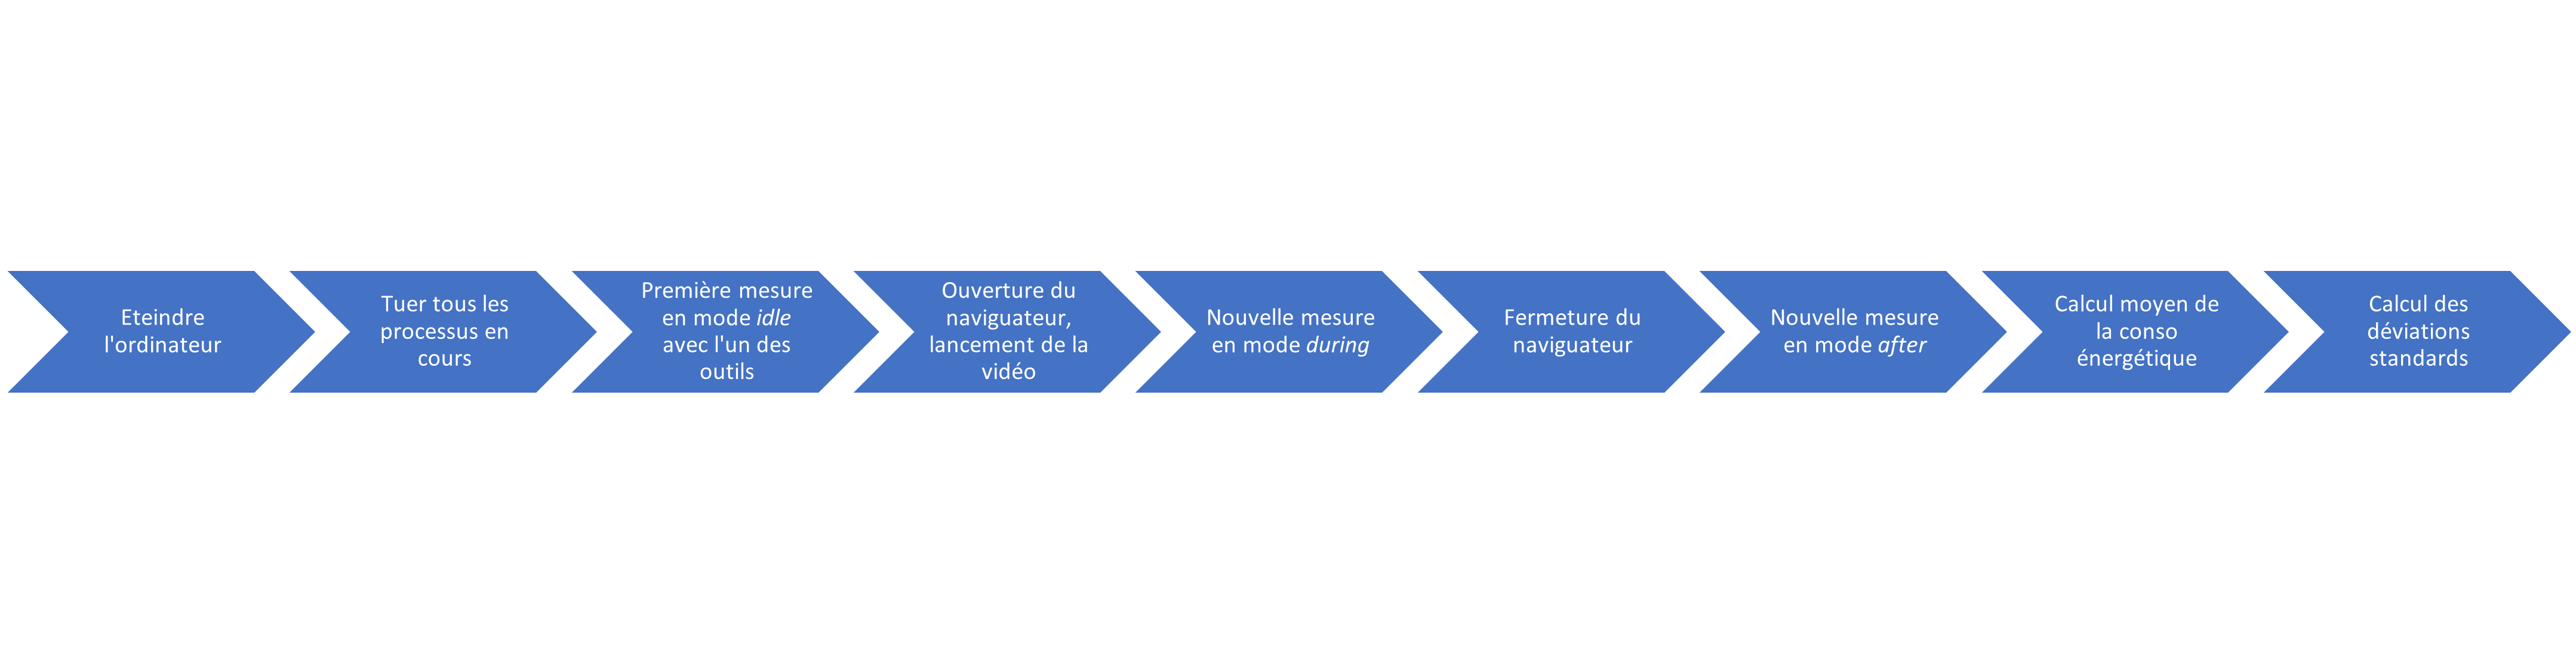
\includegraphics[width=1\linewidth]{res//graph/process.png}
    \caption{Processus de l'expérience}
    \label{fig:experience-process}
\end{figure}



\subsection{Description des scénarios de test (lecture de vidéo sur différents navigateurs)}

Nous avons entrepris des tests exhaustifs pour évaluer la consommation d'énergie lors de la lecture de vidéos, en effectuant des mesures avant, pendant, et après la lecture. Sous Windows, nous avons comparé Chrome et Edge à l'aide d'Intel Power Gadget. Sur Linux, les tests ont inclus Firefox et Chrome, avec l'utilisation d'un wattmètre, ainsi que des outils logiciels tels que PowerSpy CLI, PowerSpy2, et PowerJoular. Ces mesures couvrant l'avant, le pendant, et l'après de la lecture fournissent une perspective complète sur la performance énergétique, permettant aux utilisateurs de prendre des décisions éclairées en fonction de leurs préférences et des exigences énergétiques de leurs systèmes.

\chapter{\centering Résultats}
\subsection{Sur Windows (Intel Power Gadget)}
Sur Windows nous avons réalisé une expérience en utilisant Intel Power Gadget. Cet outil, développé par Intel et qui est maintenant obsolète (remplacé par Intel® Performance Counter Monitor) est un outil qui permet de mesurer la consommation, de chaque composant dans l'ordinateur et nous nous intéressons ici au CPU ainsi qu'à ses composants..

\begin{figure}[H]
    \centering
    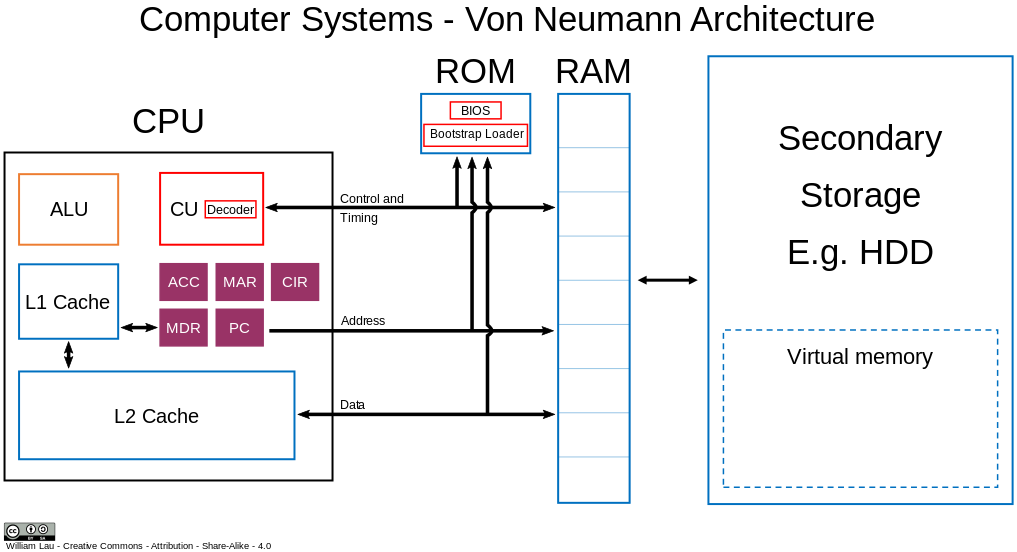
\includegraphics[width=1\linewidth]{res//CPT-Von_neumann_architecture.svg.png}
    \caption{CPU diagram}
    \label{fig:cpu_diagram}
\end{figure}

Sur toutes les variables que nous donne ce logiciel, nous avons choisis d'étudier stastistiquement les suivantes:
\textbf{Variables X}
\begin{itemize}
    \item CPU Utilization(\%)	
    \item Cumulative Processor Energy\_0(Joules)
    \item Cumulative IA Energy\_0(Joules)
    \item Cumulative DRAM Energy\_0(Joules)
    \item Cumulative GT Energy\_0(Joules)
\end{itemize}

\textbf{Variable Y : } System Time (timestap)

Nous avons choisis de prendre les différentes variables cumulatives en Joules pour exprimer l'énergie consommé et pour la variable X la variable de temps qui est le System Time. Comme ça nous pouvons analyser l'évolution de l'énergie par rapport au temps.

\subsubsection{Chrome}
\label{subsubsec:chrome_ipg}
\begin{figure}[H]
    \centering
    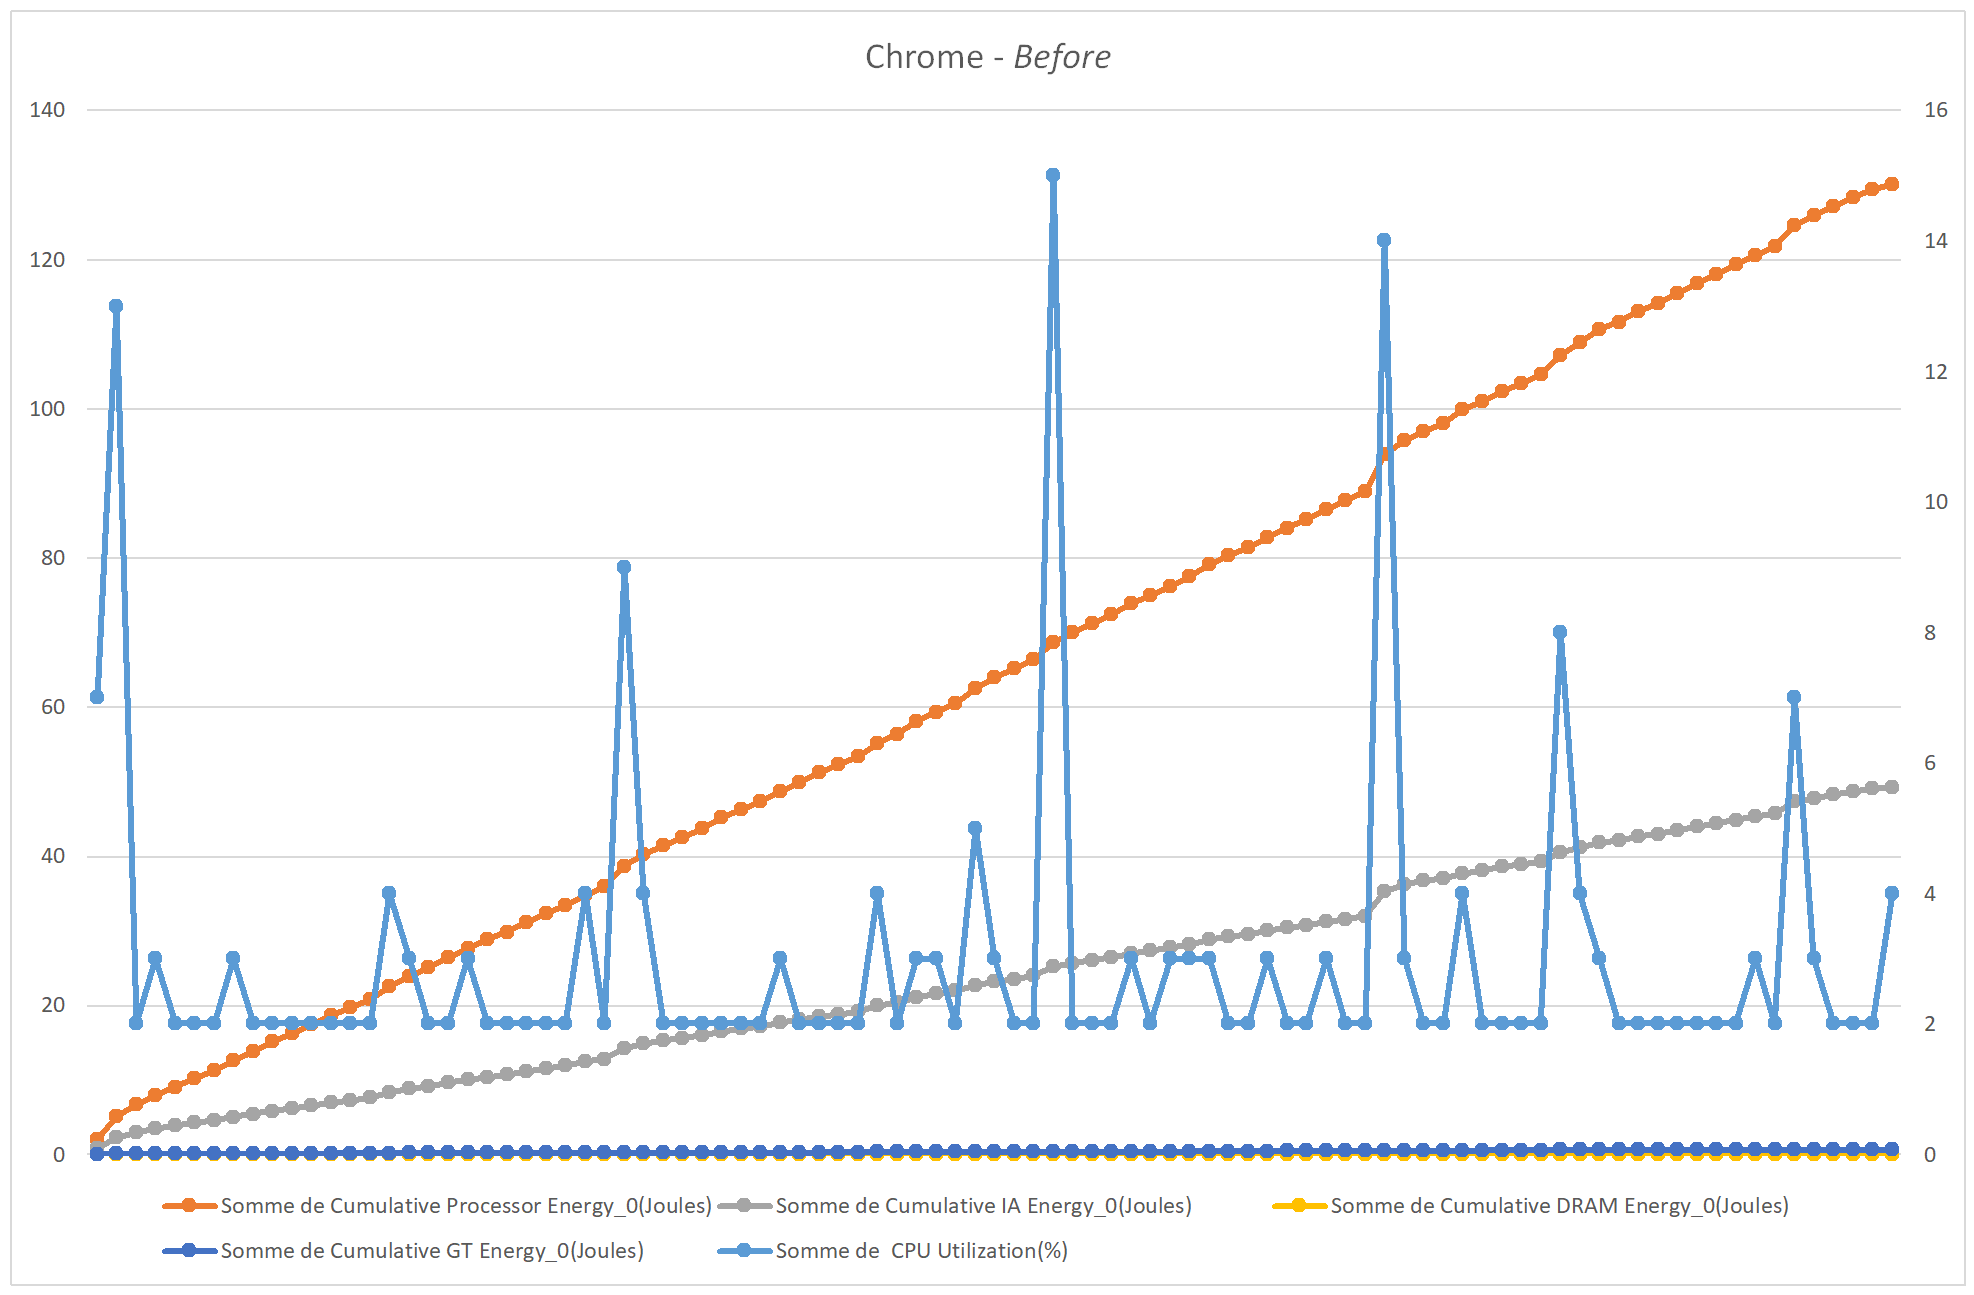
\includegraphics[width=1\linewidth]{res//graph/IntelPowerGadget/chrome-before.png}
    \caption{Intel Power Gadget - Chrome - \textit{before}}
    \label{fig:ipg_chrome-before}
\end{figure}
\begin{figure}[H]
    \centering
    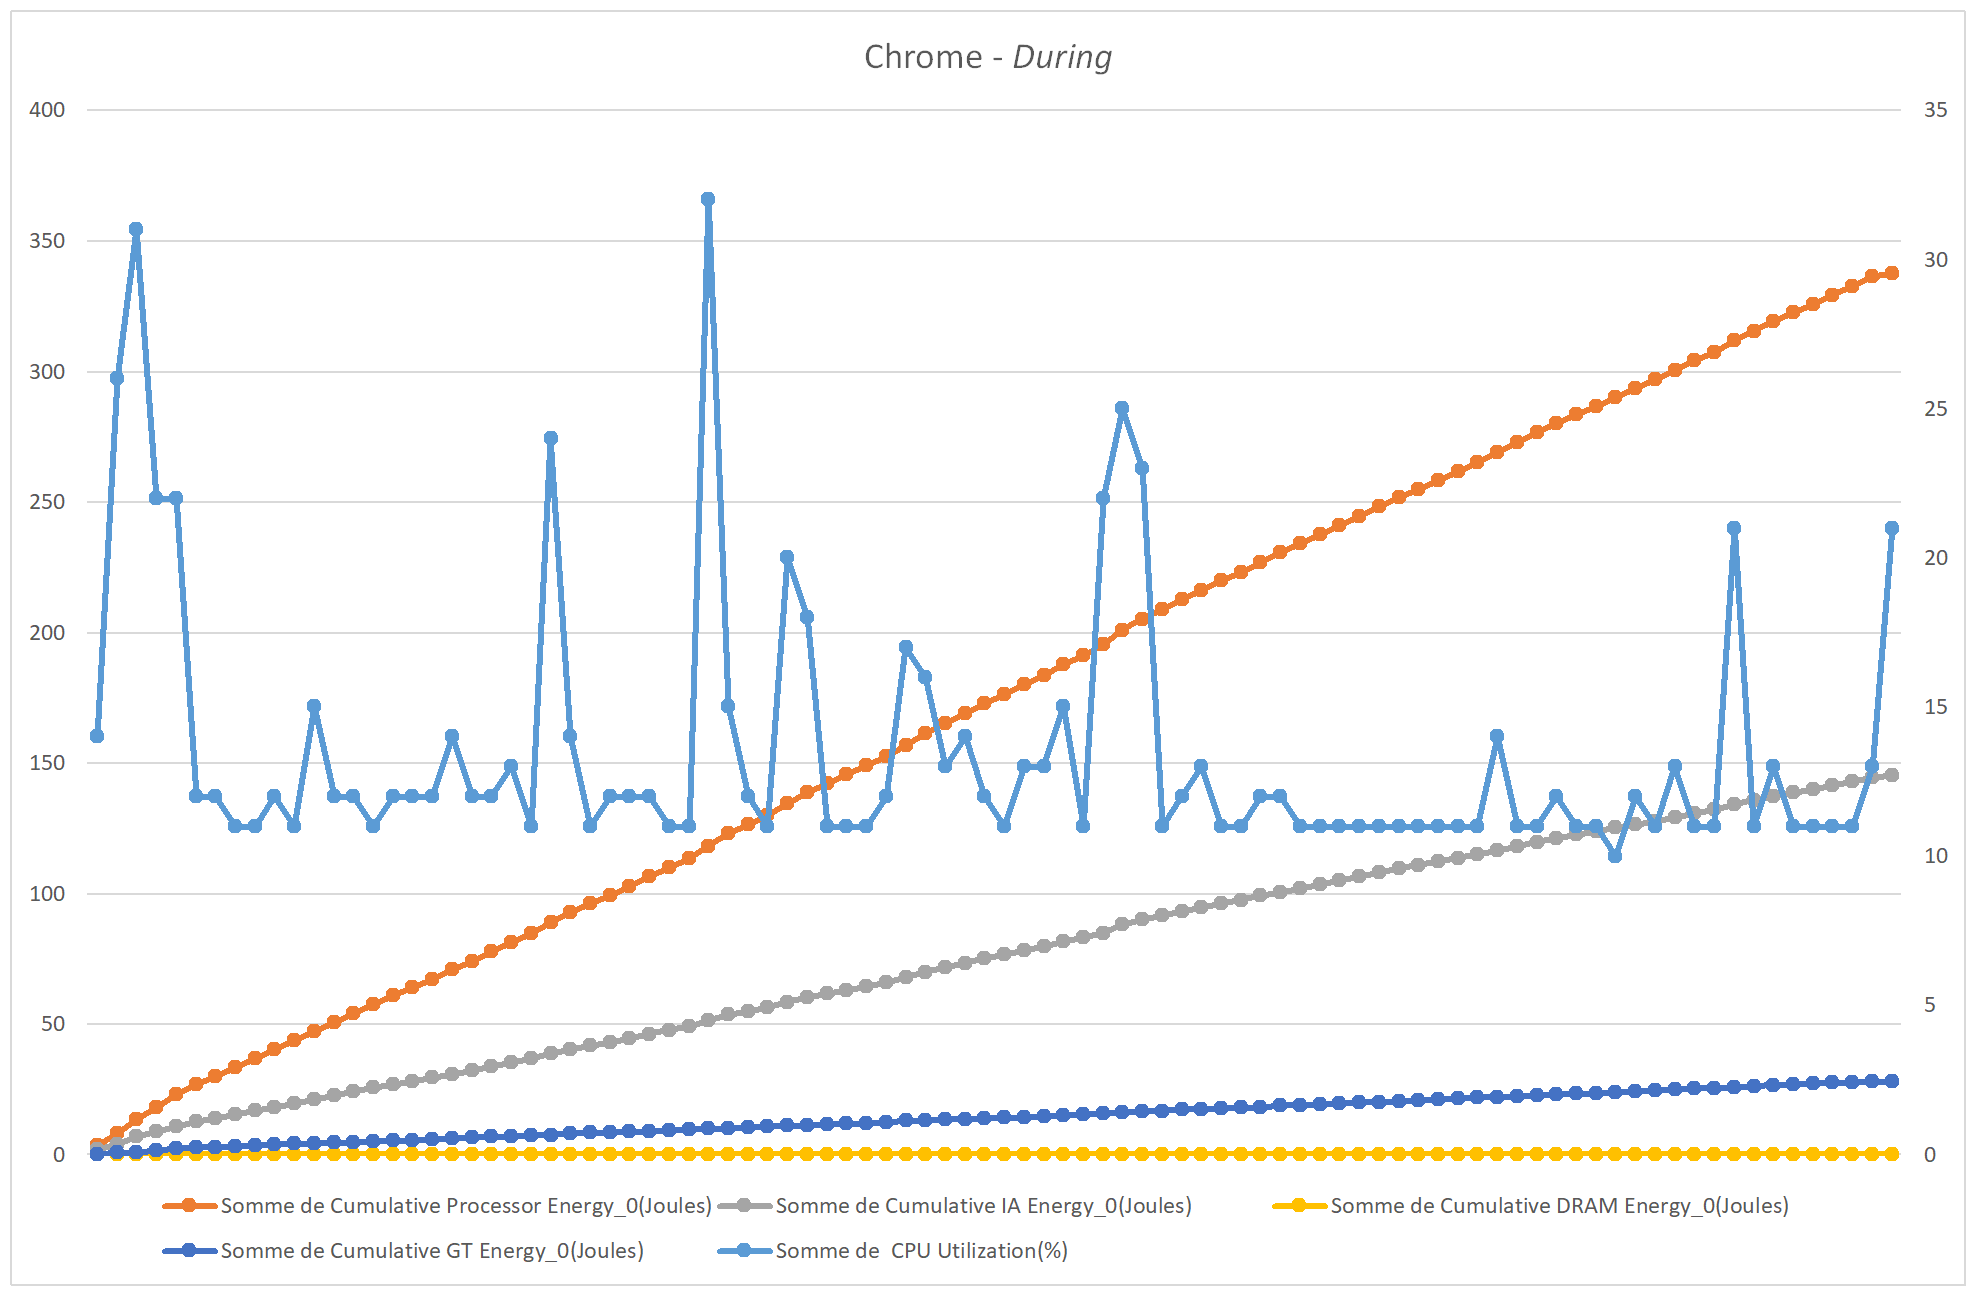
\includegraphics[width=1\linewidth]{res//graph/IntelPowerGadget/chrome-during.png}
    \caption{Intel Power Gadget - Chrome - \textit{during}}
    \label{fig:ipg_chrome-during}
\end{figure}
\begin{figure}[H]
    \centering
    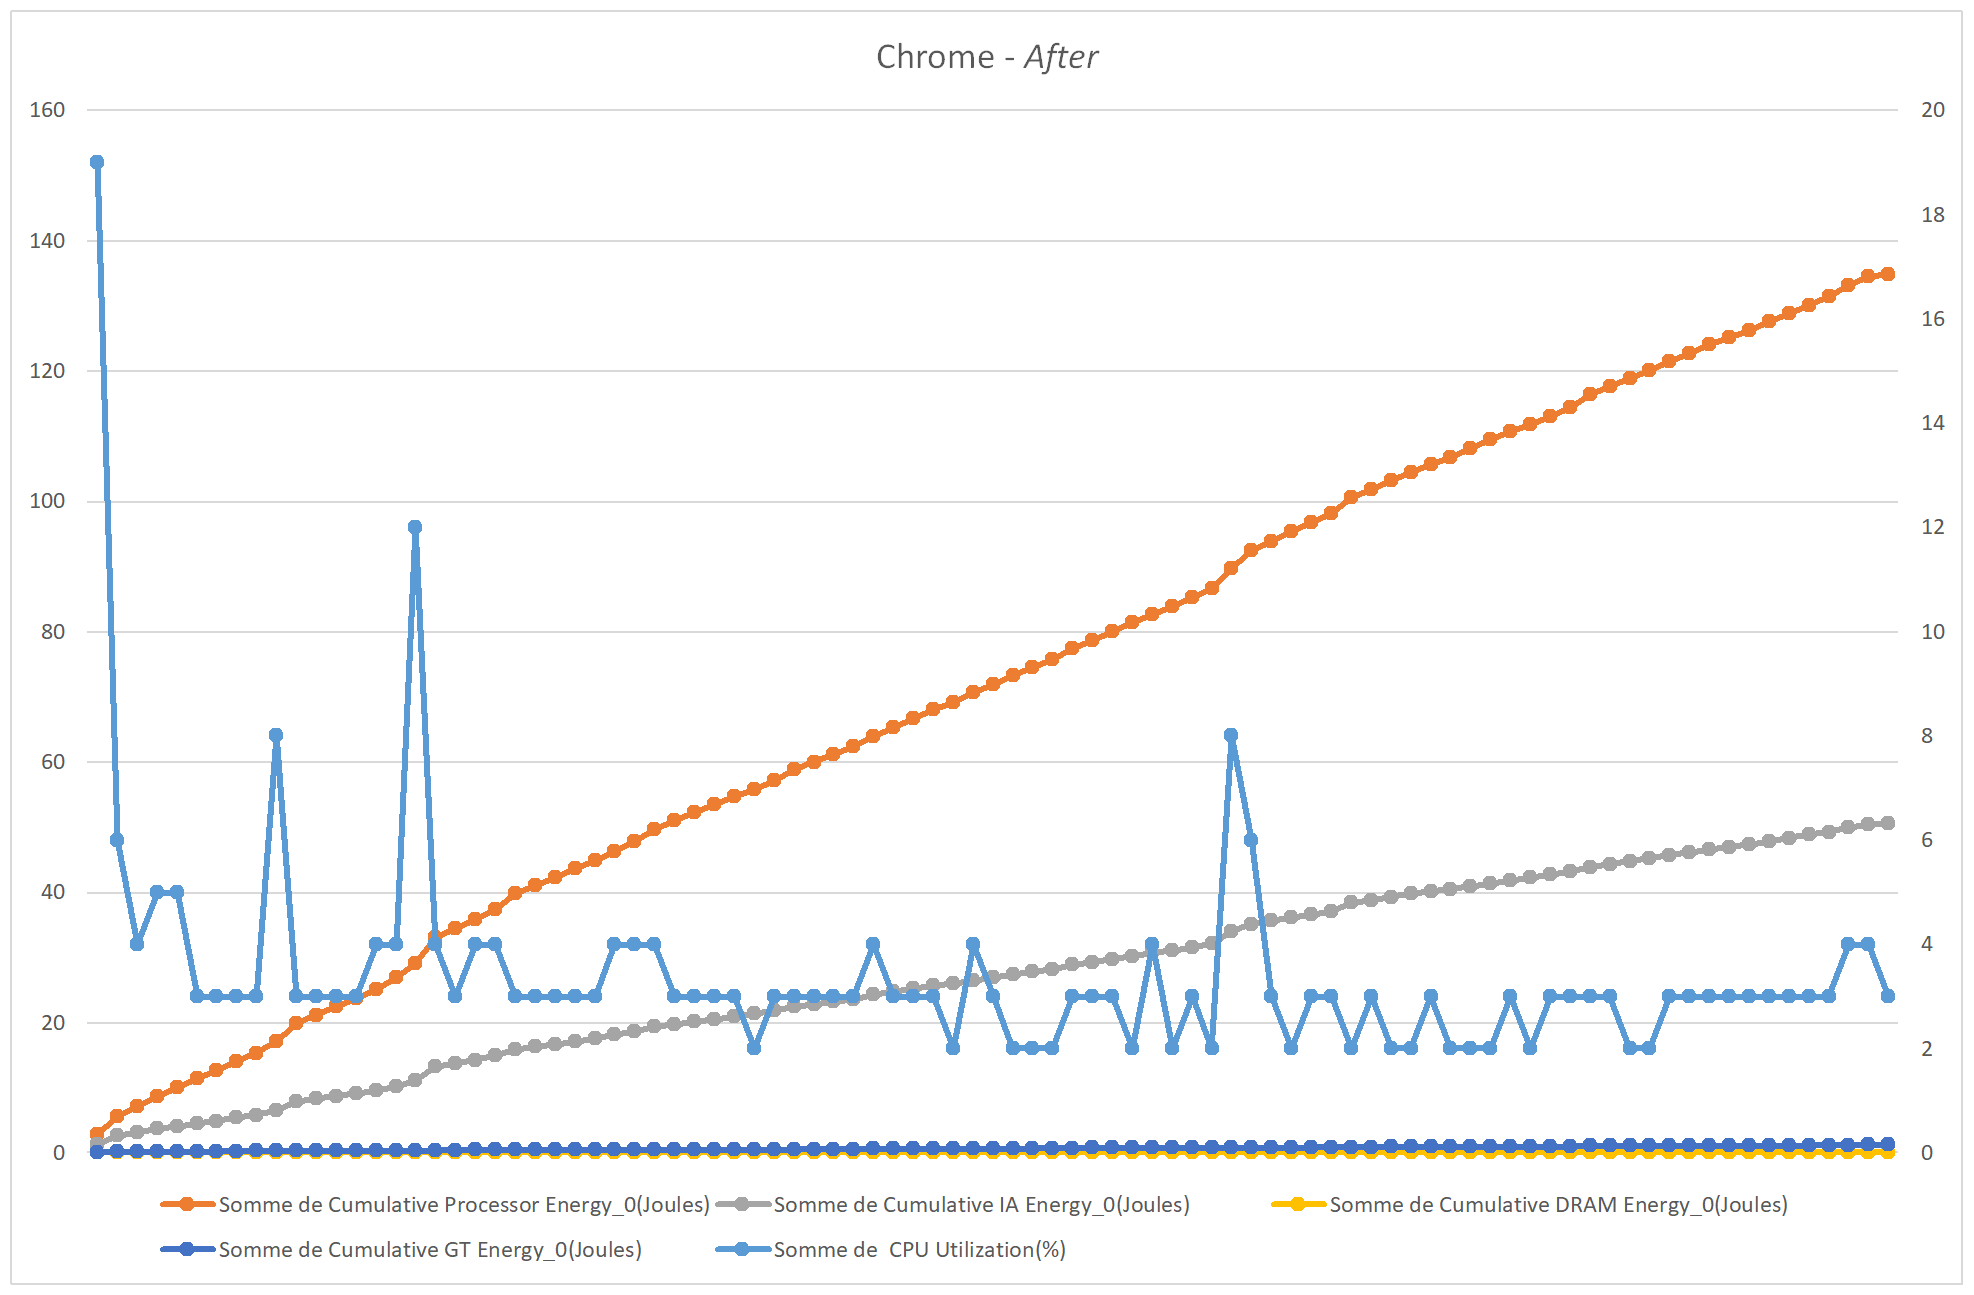
\includegraphics[width=1\linewidth]{res//graph/IntelPowerGadget/chrome-after.png}
    \caption{Intel Power Gadget - Chrome - \textit{after}}
    \label{fig:ipg_chrome-after}
\end{figure}
Lors de la visualisation de la vidéo, le CPU utilise jusqu'à 350 Joules environ et son taux d'utilisation varie de 10 à 35\% (alors que au repos, le processus varie entre 2 et 16\%.
Bien entendu, il est totalement logique que la consomation augmente lors d'une utilisation intensive (ou plus intensive que au repos) du CPU, par exemple en lisant une vidéo.
Avant et après la lecture, le CPU retourne à une consommation "normale", chose que nous verrons sur l'expérience de Edge mais qui n'est pas commun.


\subsubsection{Edge}
\begin{figure}[H]
    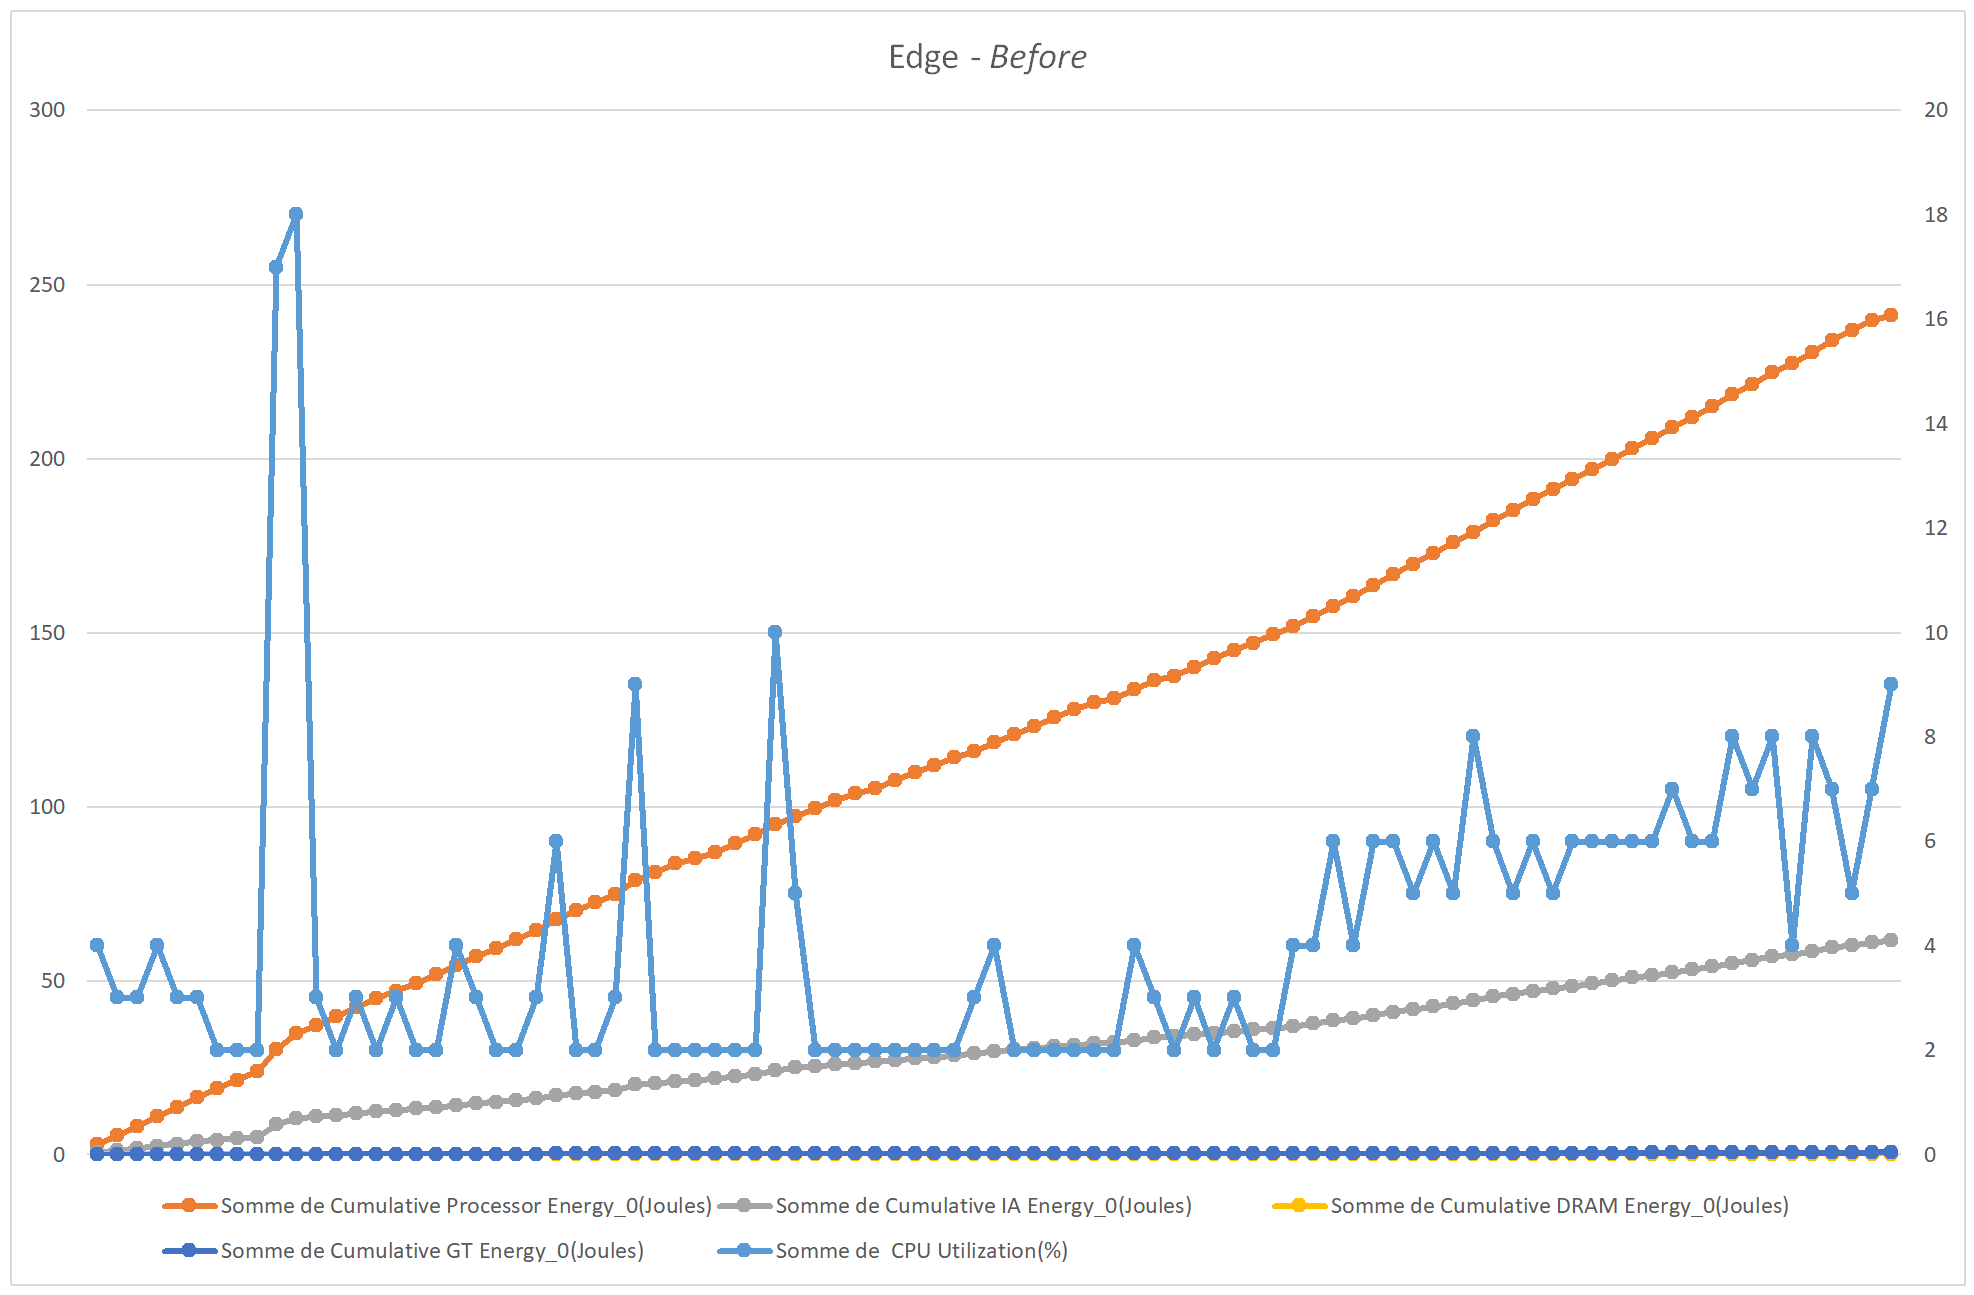
\includegraphics[width=1\linewidth]{res//graph/IntelPowerGadget/edge-before.png}
    \caption{Intel Power Gadget - Edge - \textit{before}}
    \label{fig:ipg_edge-before}
\end{figure}
\begin{figure}[H]
    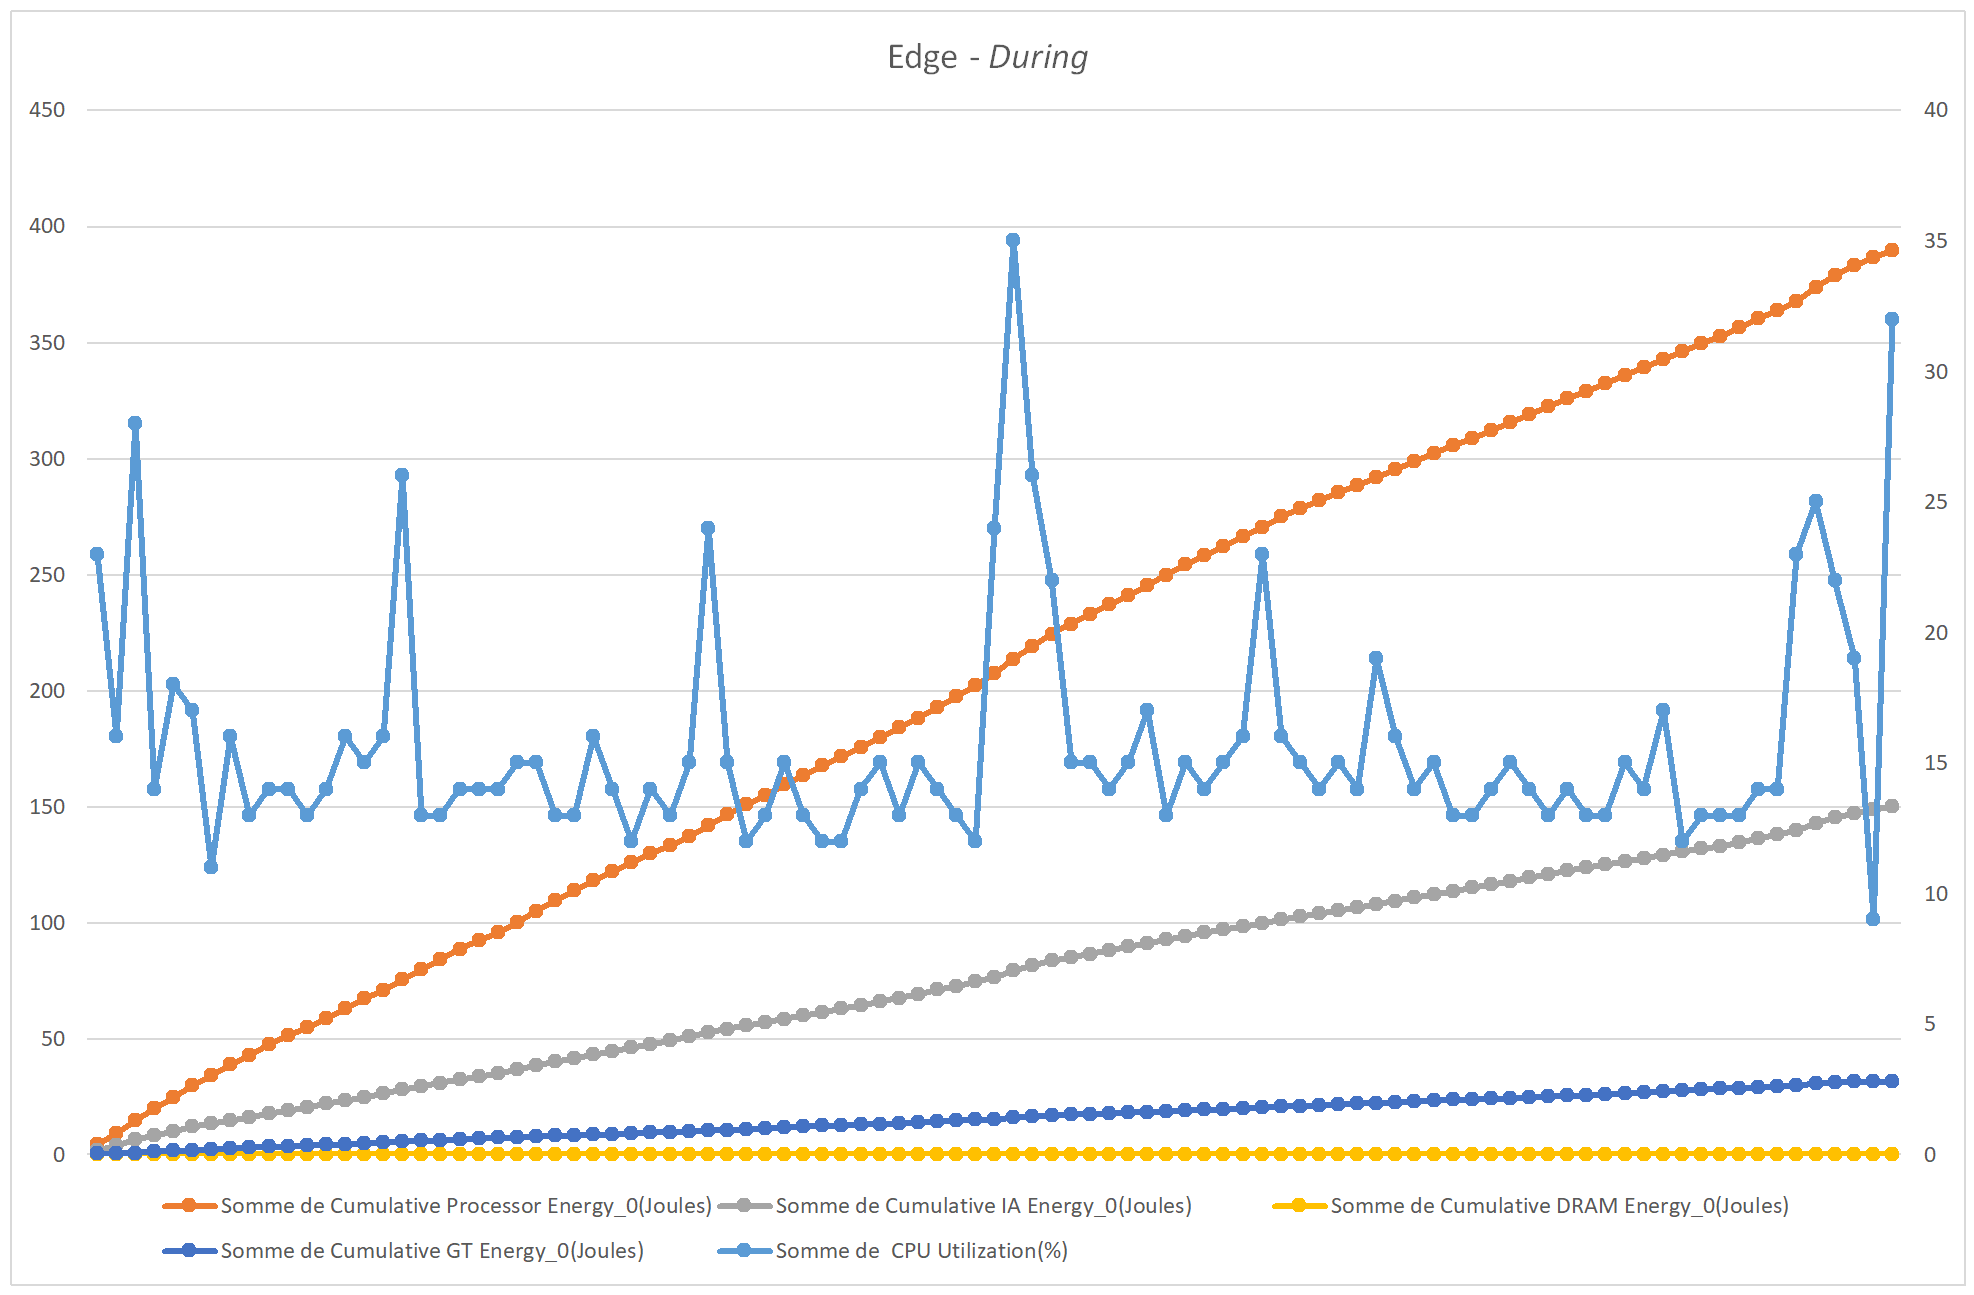
\includegraphics[width=1\linewidth]{res//graph/IntelPowerGadget/edge-during.png}
    \caption{Intel Power Gadget - Edge - \textit{during}}
    \label{fig:ipg_edge-during}
\end{figure}
\begin{figure}[H]
    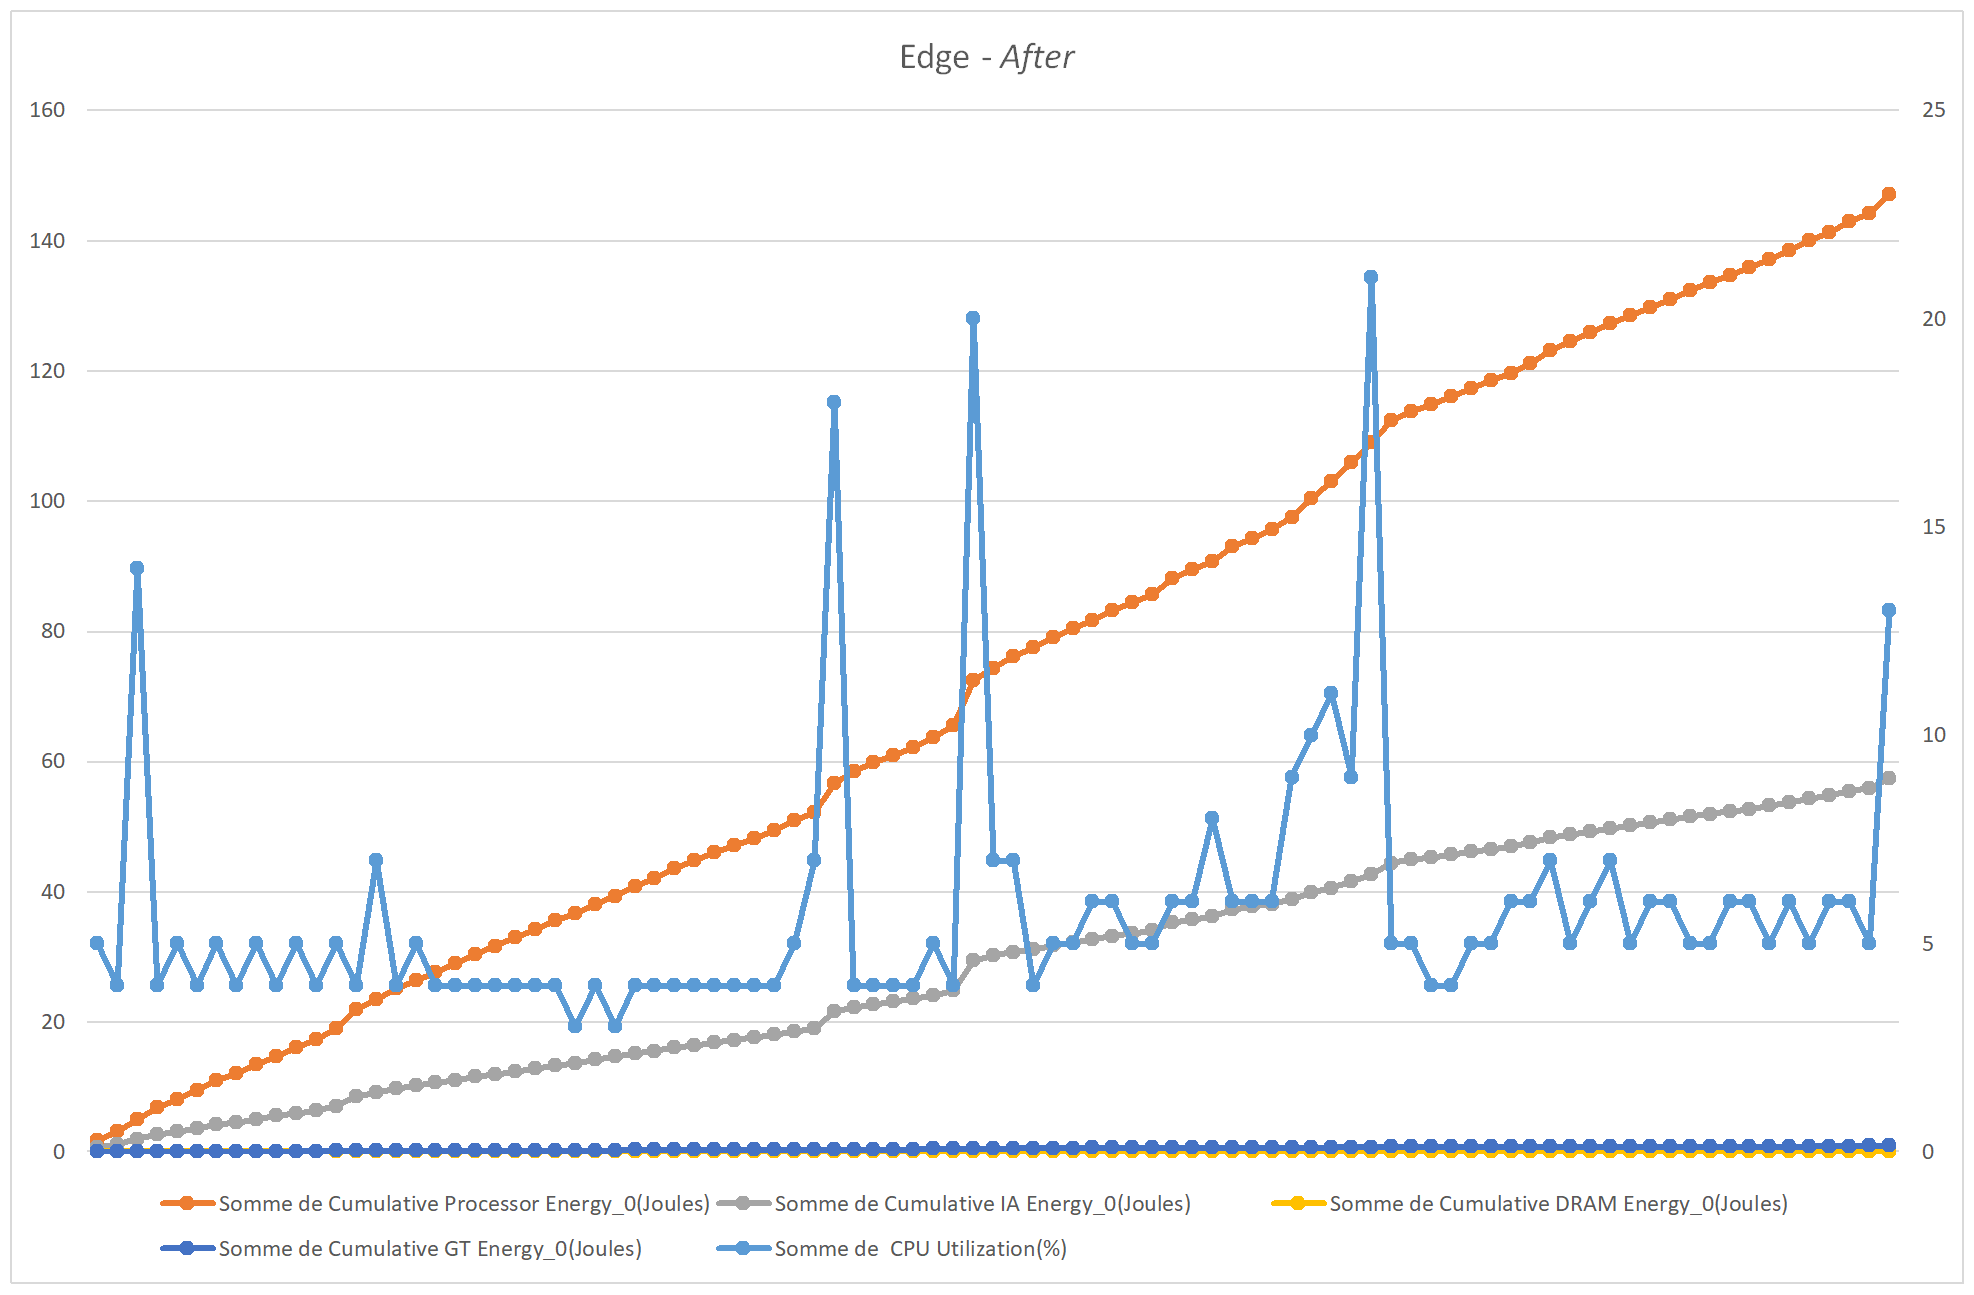
\includegraphics[width=1\linewidth]{res//graph/IntelPowerGadget/edge-after.png}
    \caption{Intel Power Gadget - Edge - \textit{after}}
    \label{fig:ipg_edge-after}
\end{figure}

Une chose intéressante à noter sur l'expérience faite sur Edge est la présence des différents pics d'activités sur l'énergie consommée par la DRAM APRÈS la vision de la vidéo quand le pourcentage d'utilisation du CPU augmente. Or, ces pics ne sont pas perçu lors de l'expérience faites sur Chrome. 
Un autre point à voir sont les échelles qui sont semblable entre Chrome et Edge. 
De plus, après la lecture de la vidéo, edge continue de consommer plus que son état initial \textit{idle}. Le CPU consomme moins que lors de la visualisation de la vidéo, mais reste très bas.

\paragraph{
\textbf{Différences notables}\newline
Nous pouvons voir une certaine différence entre l'utilisation des ressource du CPU entre les deux naviguateurs et donc une améliroation de la consomation d'énergie du CPU lors de l'utilisation de Chrome.
Même si les ordres de grandeurs sont les mêmes et qu'une utilisation plus intensive est notable pour les deux naviguateurs lors de la lecture de la vidéo. 
Cependant, sur tous les aspects il est clair que Chrome utilise mieux les ressources et engendre donc moins de consomation énergétique, que ce soit au repos ou en action. Edge tournant à environ 7\% de l'utilisation du CPU au repos contre 2\% pour Chrome. Ce qui représente pour la consomation globale en Joules du CPU un maximum de 250J pour Edge contre 140J pour Chrome. Quand à la stabilité sur l'utilisation du CPU pendant la lecture de la vidéo, Edge a beaucoup plus de mal à rester constant et stable, ce qui engendre un surcoup de la consommation (le CPU est plus intensément utilisé), passant de pic à 35\% d'utilisation à 15\%, et contenant beaucoup plus de pics aléatoire. Chrome possède beaucoup moins de ces spécularité et les sauts majeurs sont beaucoup moins importants. 
}

\subsection{Linux}

Sur Linux nous avons eu la chance de pouvoir travailler sur beaucoup plus d'expérience avec plus d'outils de mesure. 
Nous avons pu connecter un Wattmètre à notre PC Linux où nous lancerons les vidéos, puis, depuis un autre ordinateur, nous nous connecterons sur le wattmètre en bluetooth pour réaliser les mesures. Comme dis précédement, les mesures ont étaient faites avec différentes outils que nous avons analysé au cas par cas et par naviguateur.

\subsubsection{PowerSpyCLI}
\label{subsubsec:powerspycli}
\begin{figure}[H]
    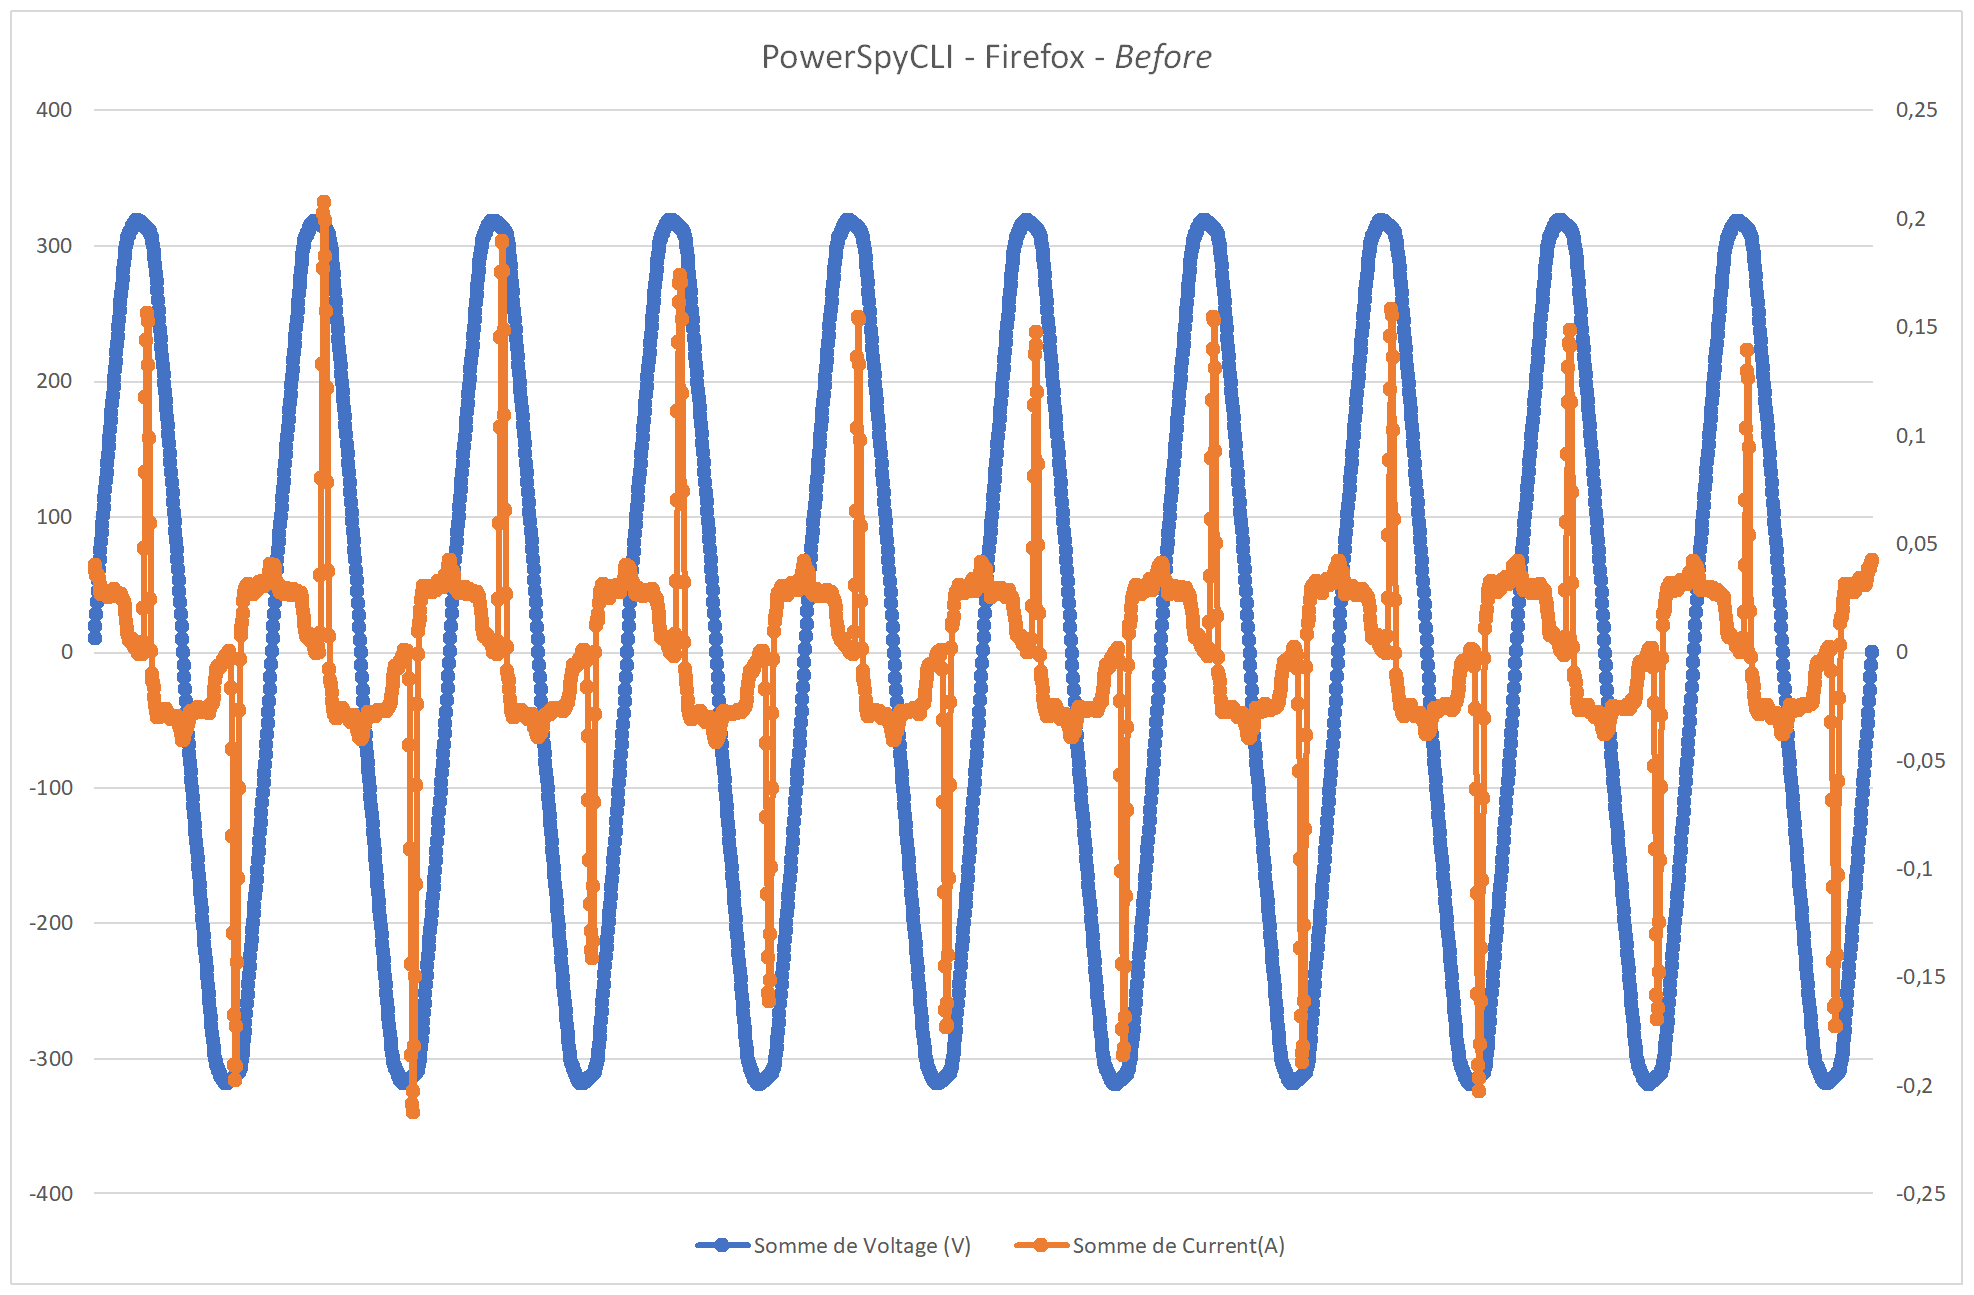
\includegraphics[width=1\linewidth]{res//graph/PowerSpyCLI/PowerSpyCLI-FF-Before.png}
    \caption{PowerSpyCLI - Firefox - \textit{before}}
    \label{fig:pscli_ff_before}
\end{figure}
\begin{figure}[H]
    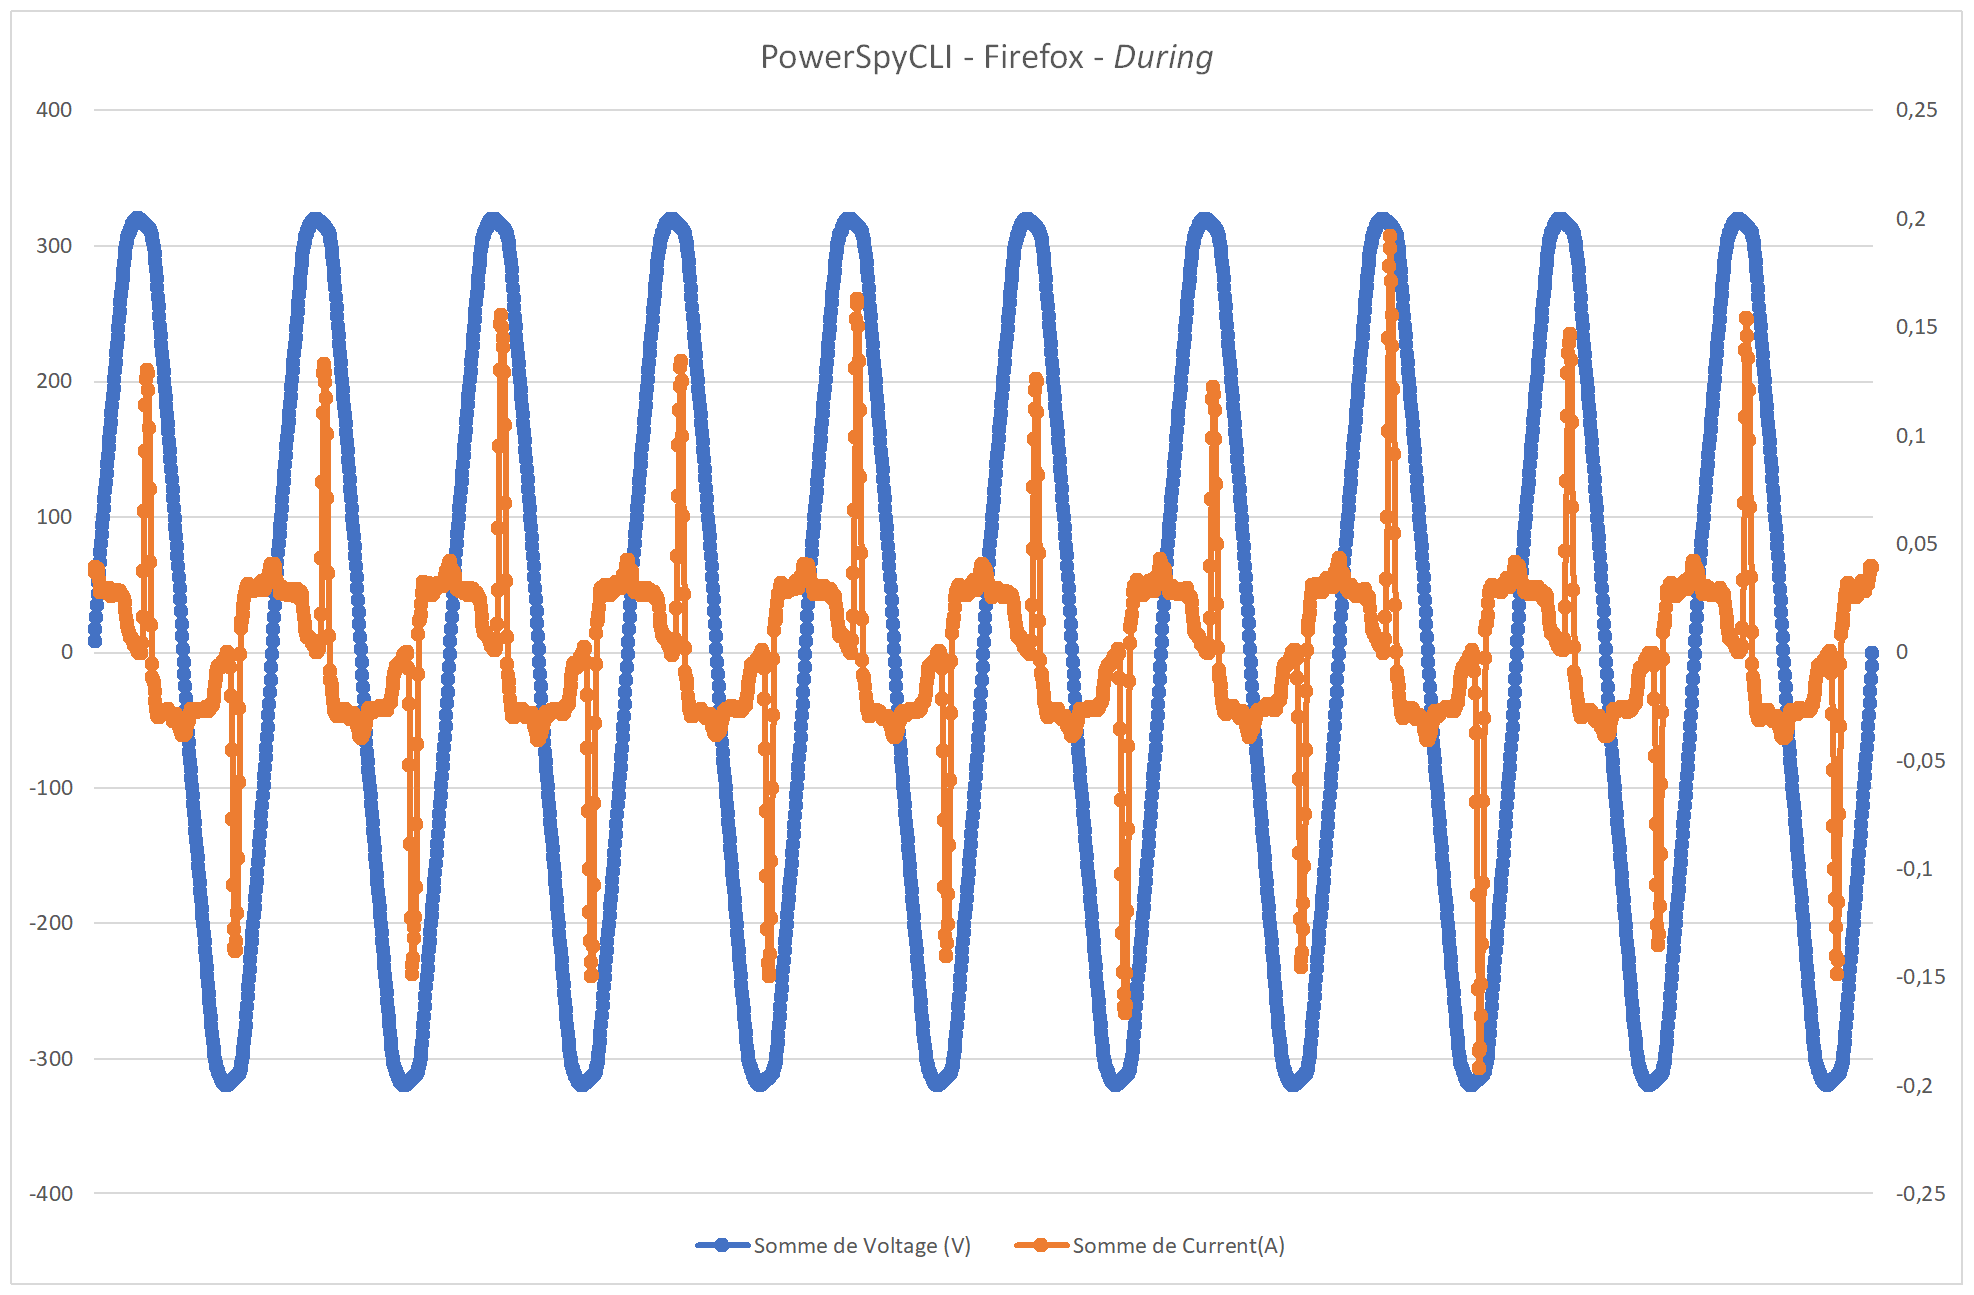
\includegraphics[width=1\linewidth]{res//graph/PowerSpyCLI/PowerSpyCLI-FF-During.png}
    \caption{PowerSpyCLI - Firefox - \textit{during}}
    \label{fig:pscli_ff_during}
\end{figure}
\begin{figure}[H]
    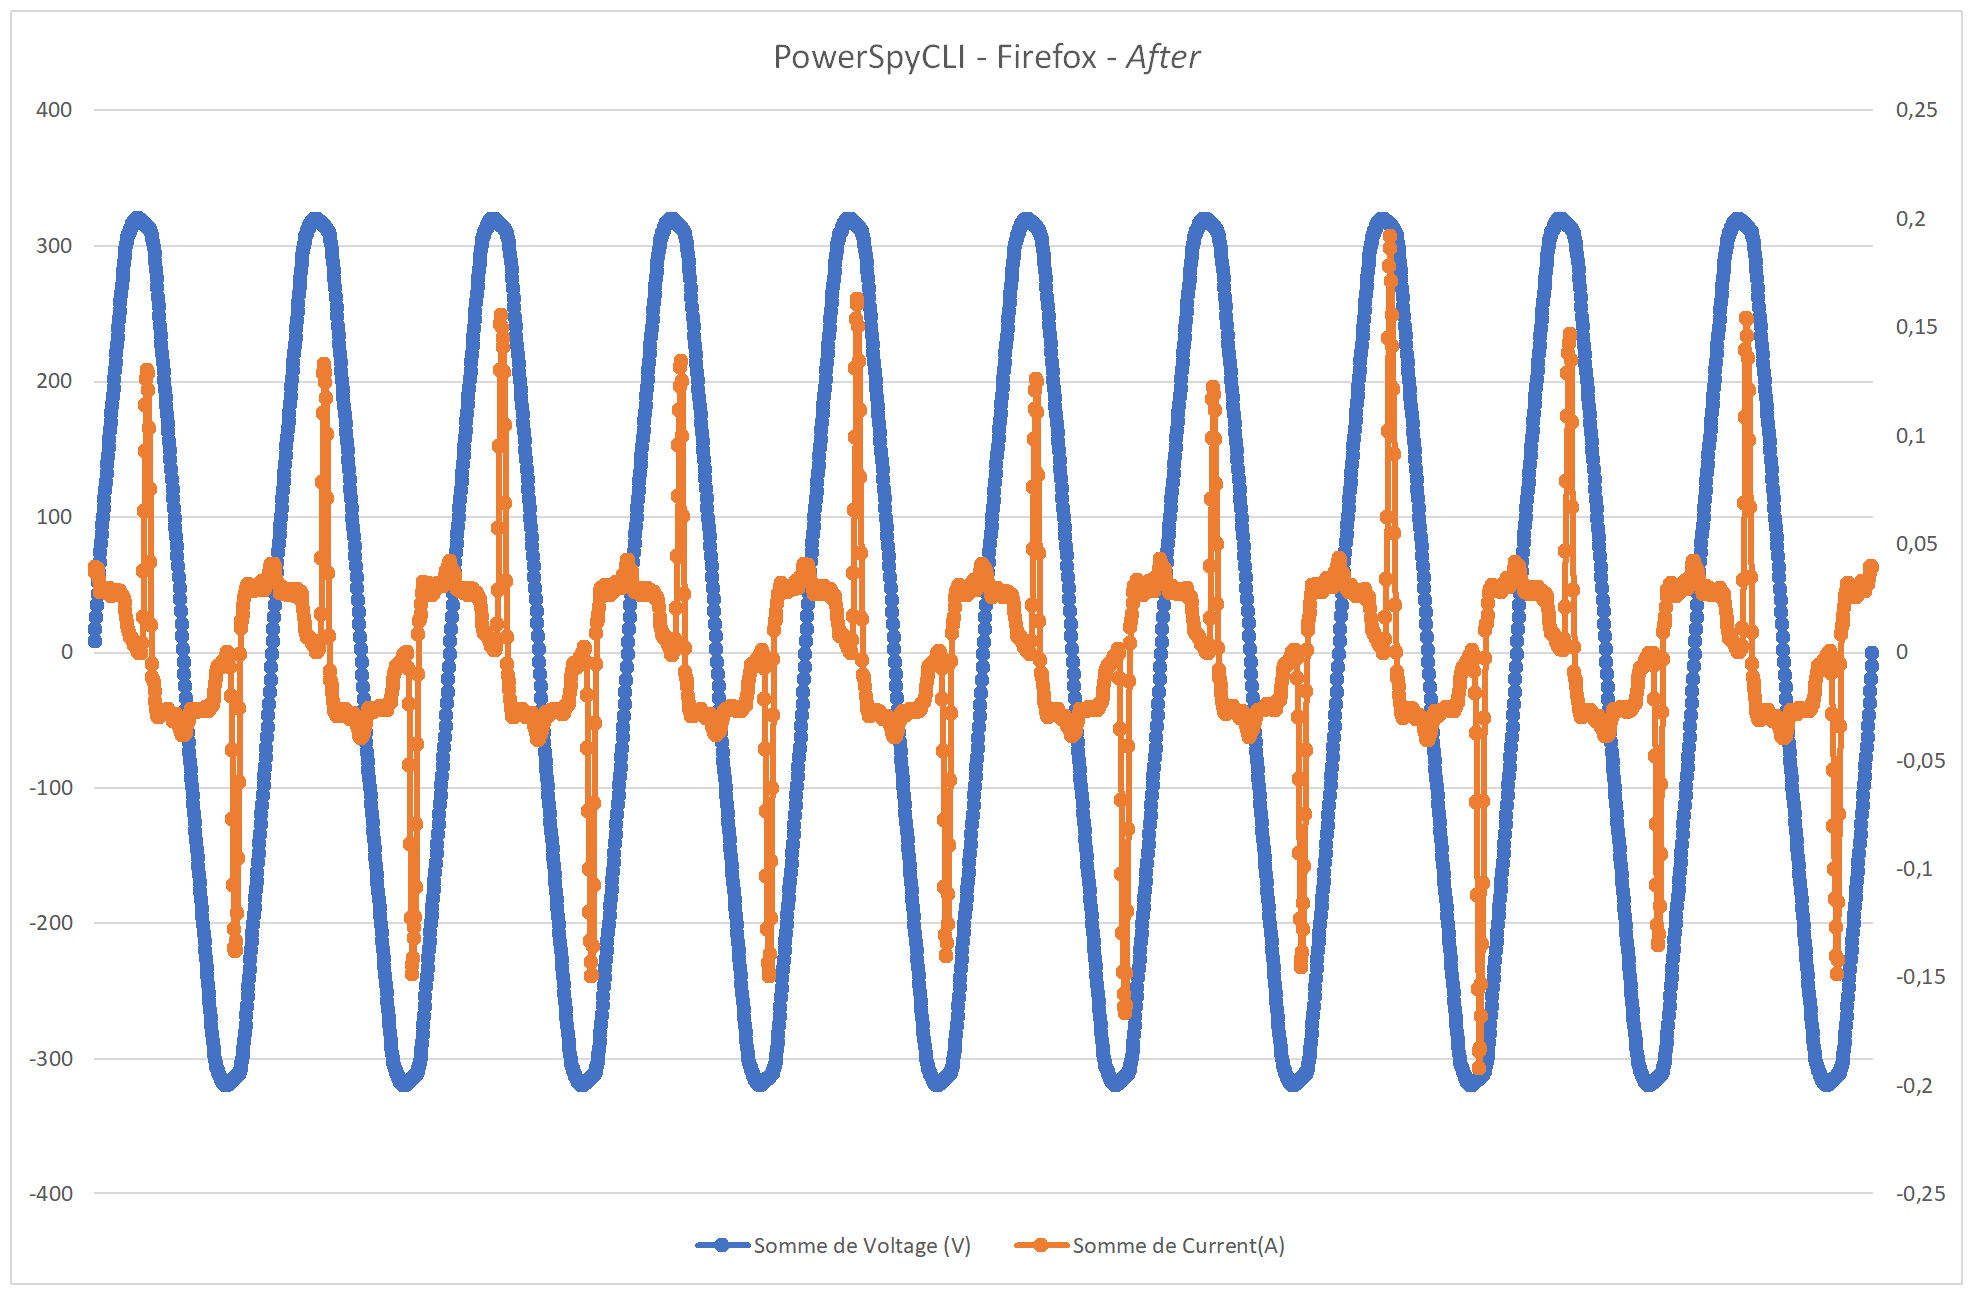
\includegraphics[width=1\linewidth]{res//graph/PowerSpyCLI/PowerSpyCLI-FF-After.png}
    \caption{PowerSpyCLI - Firefox - \textit{after}}
    \label{fig:pscli_ff_after}
\end{figure}

Pour cette première analyse nous avons voulu visualiser les données brutes directement. Nous pouvons donc voir sur ces trois différents graphiques le voltage, 230 alternatif puis les ampérage (le courant), toujours en fonction du temps. Nous remarquons, comme attendu, que le voltage reste constant dans l'alternation et le voltage en lui même, 230V. Pour le courant, nous suivons une même fonction sinusoïdale mais, à la différence du voltage, contient du bruit, très visible au niveau des pics en milieu d'alternance haute ou basse. Il n'y a pas vraiment de différence entre les trois graphiques (\textit{before, during et after} et ces pics peuvent être expliqué assez simplement au niveau physique et ingénieurie de la grille électrique en France. En effet, à chaque alternation du voltage, nous avons un pic semblable au niveau de courant. Ce changement est très fortement dû à un effet magnétique du courant lors du changement de phase. 

De plus, nous avons voulu calculer la puissance consommée pendant l'expérience en utilisant la formule suivante :
\begin{equation}
    P=V\times I
    \label{eq:puissance}
\end{equation}
Pour ces trois différents graphiques, nous avons décidé de visualiser la puissance que nous venons de calculer et le courant (en ampère) que nous avions déjà. Voici nos résultats :
\begin{figure}[H]
    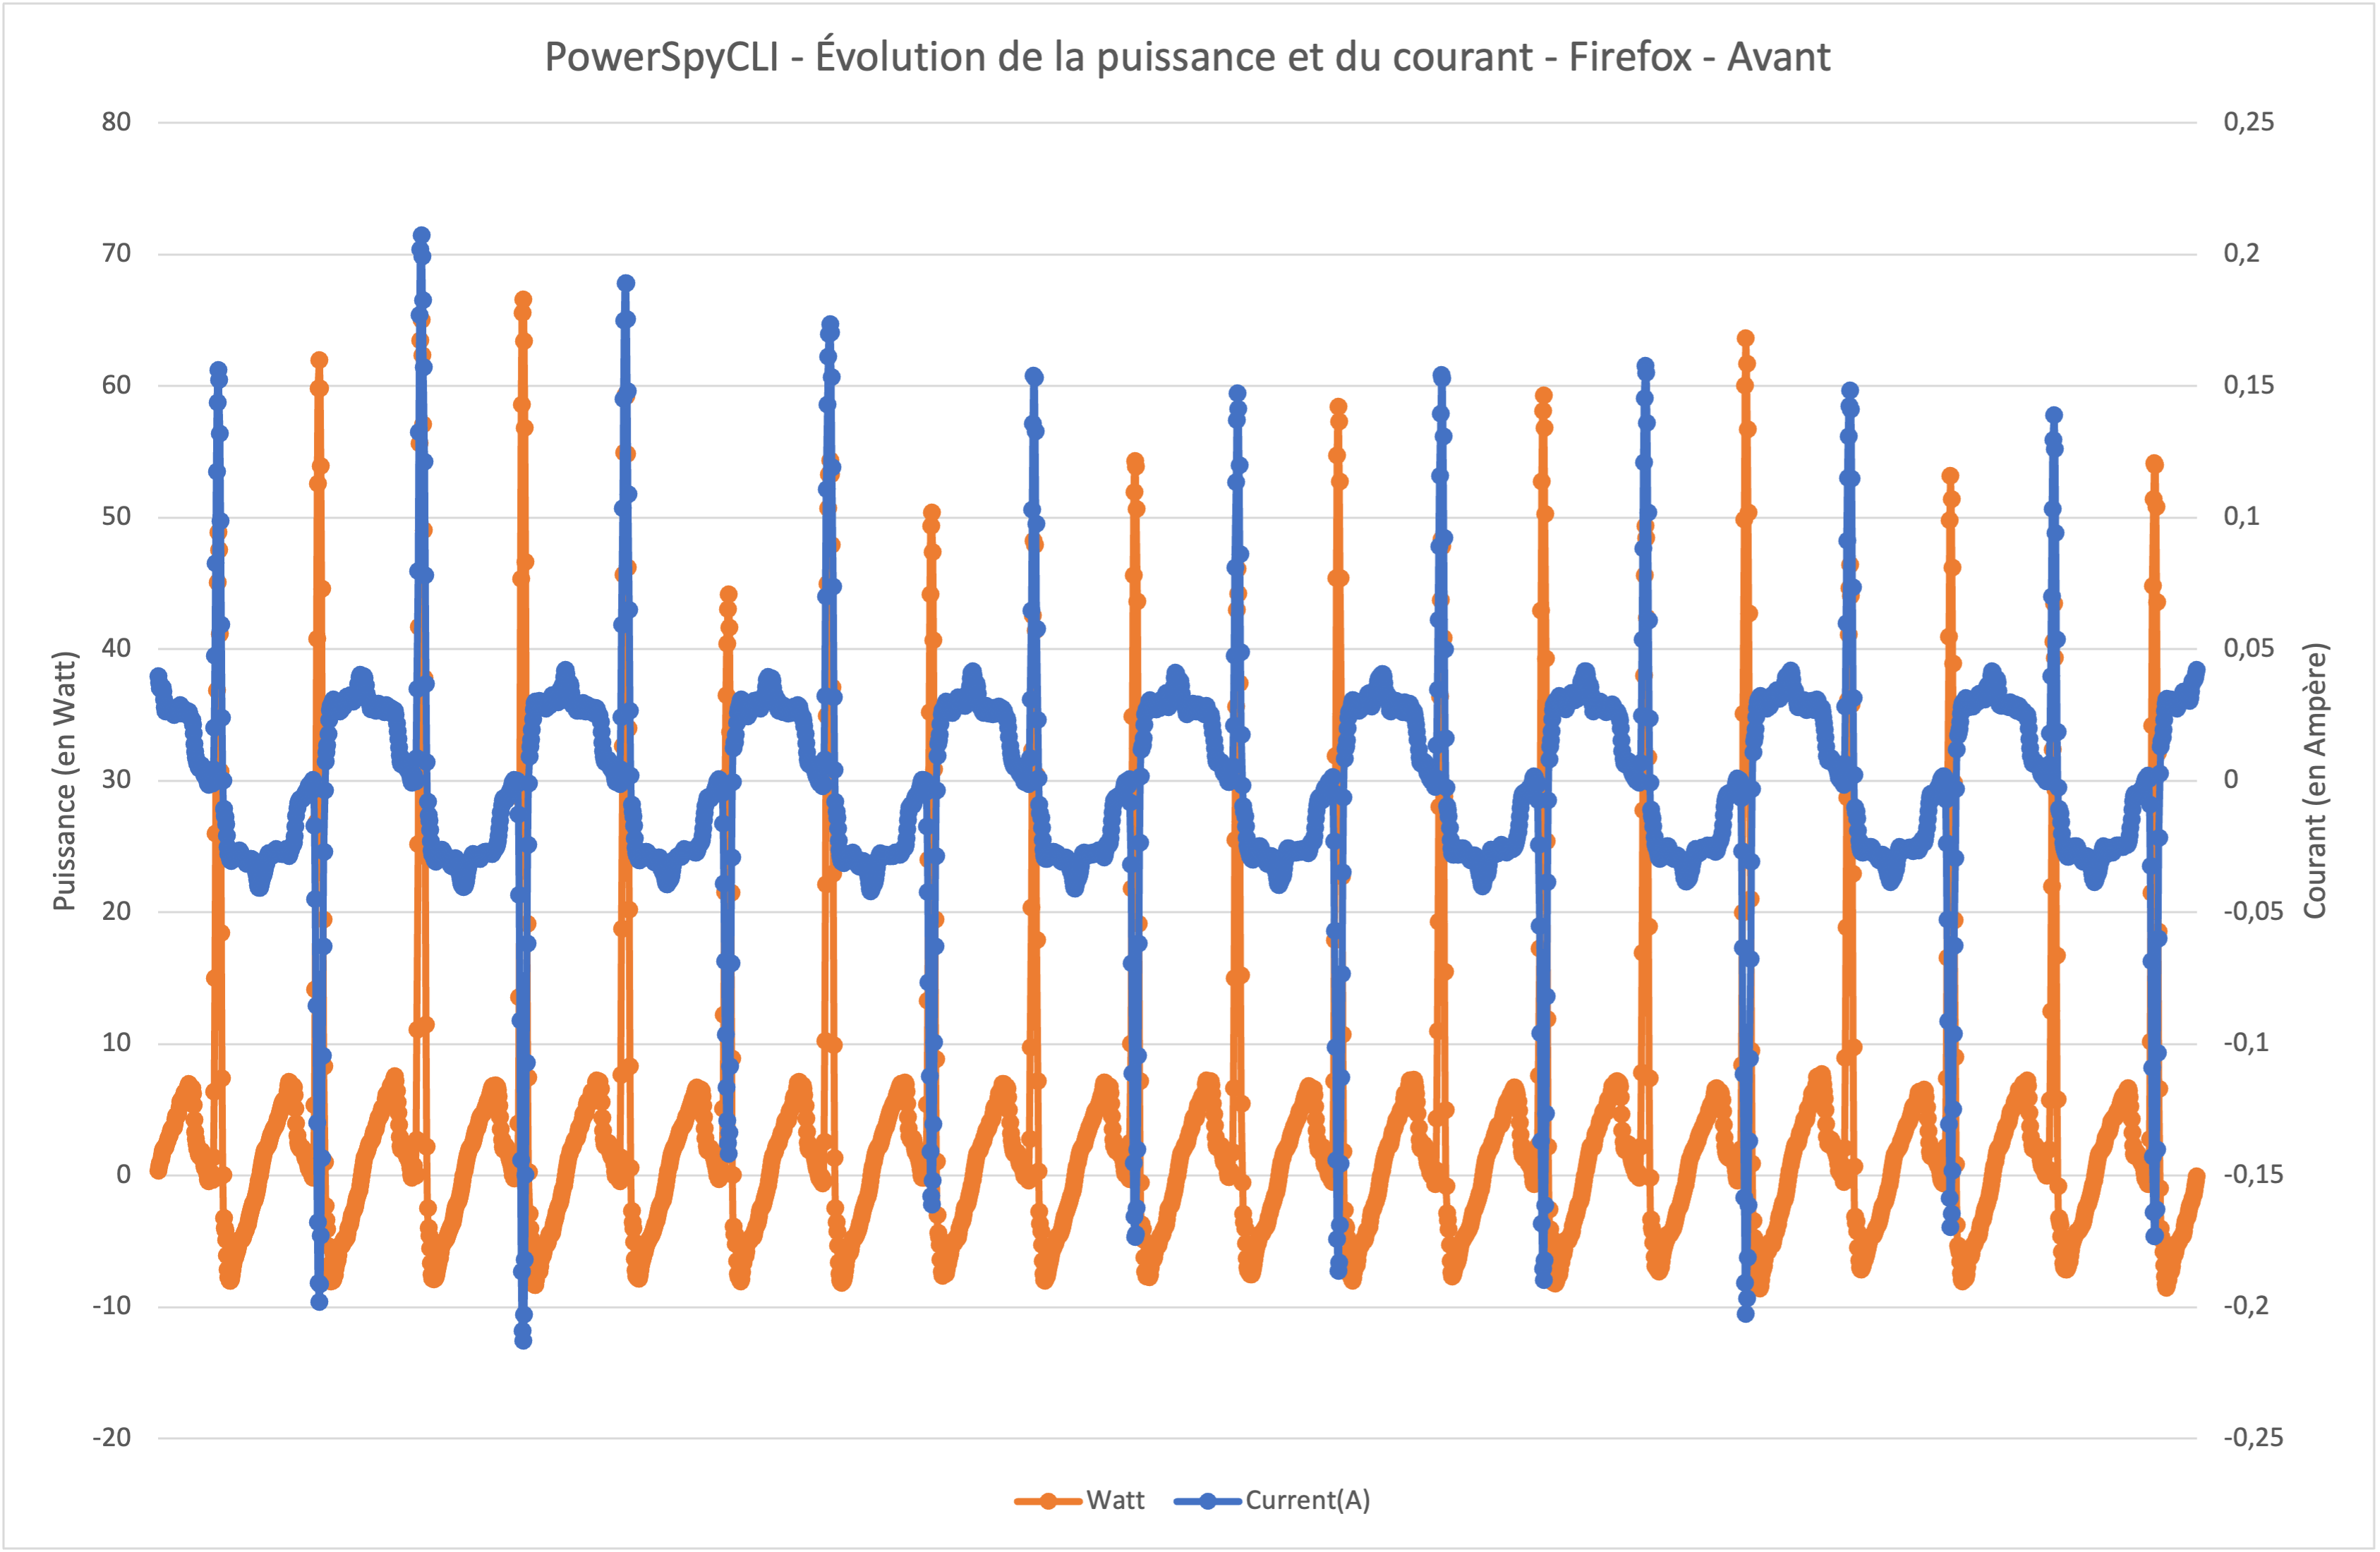
\includegraphics[width=1\linewidth]{res//graph/PowerSpyCLI/Puissance_ff_avant.png}
    \caption{PowerSpyCLI - Puissance - Firefox - \textit{after}}
    \label{fig:pscli_power_ff_after}
\end{figure}
\begin{figure}[H]
    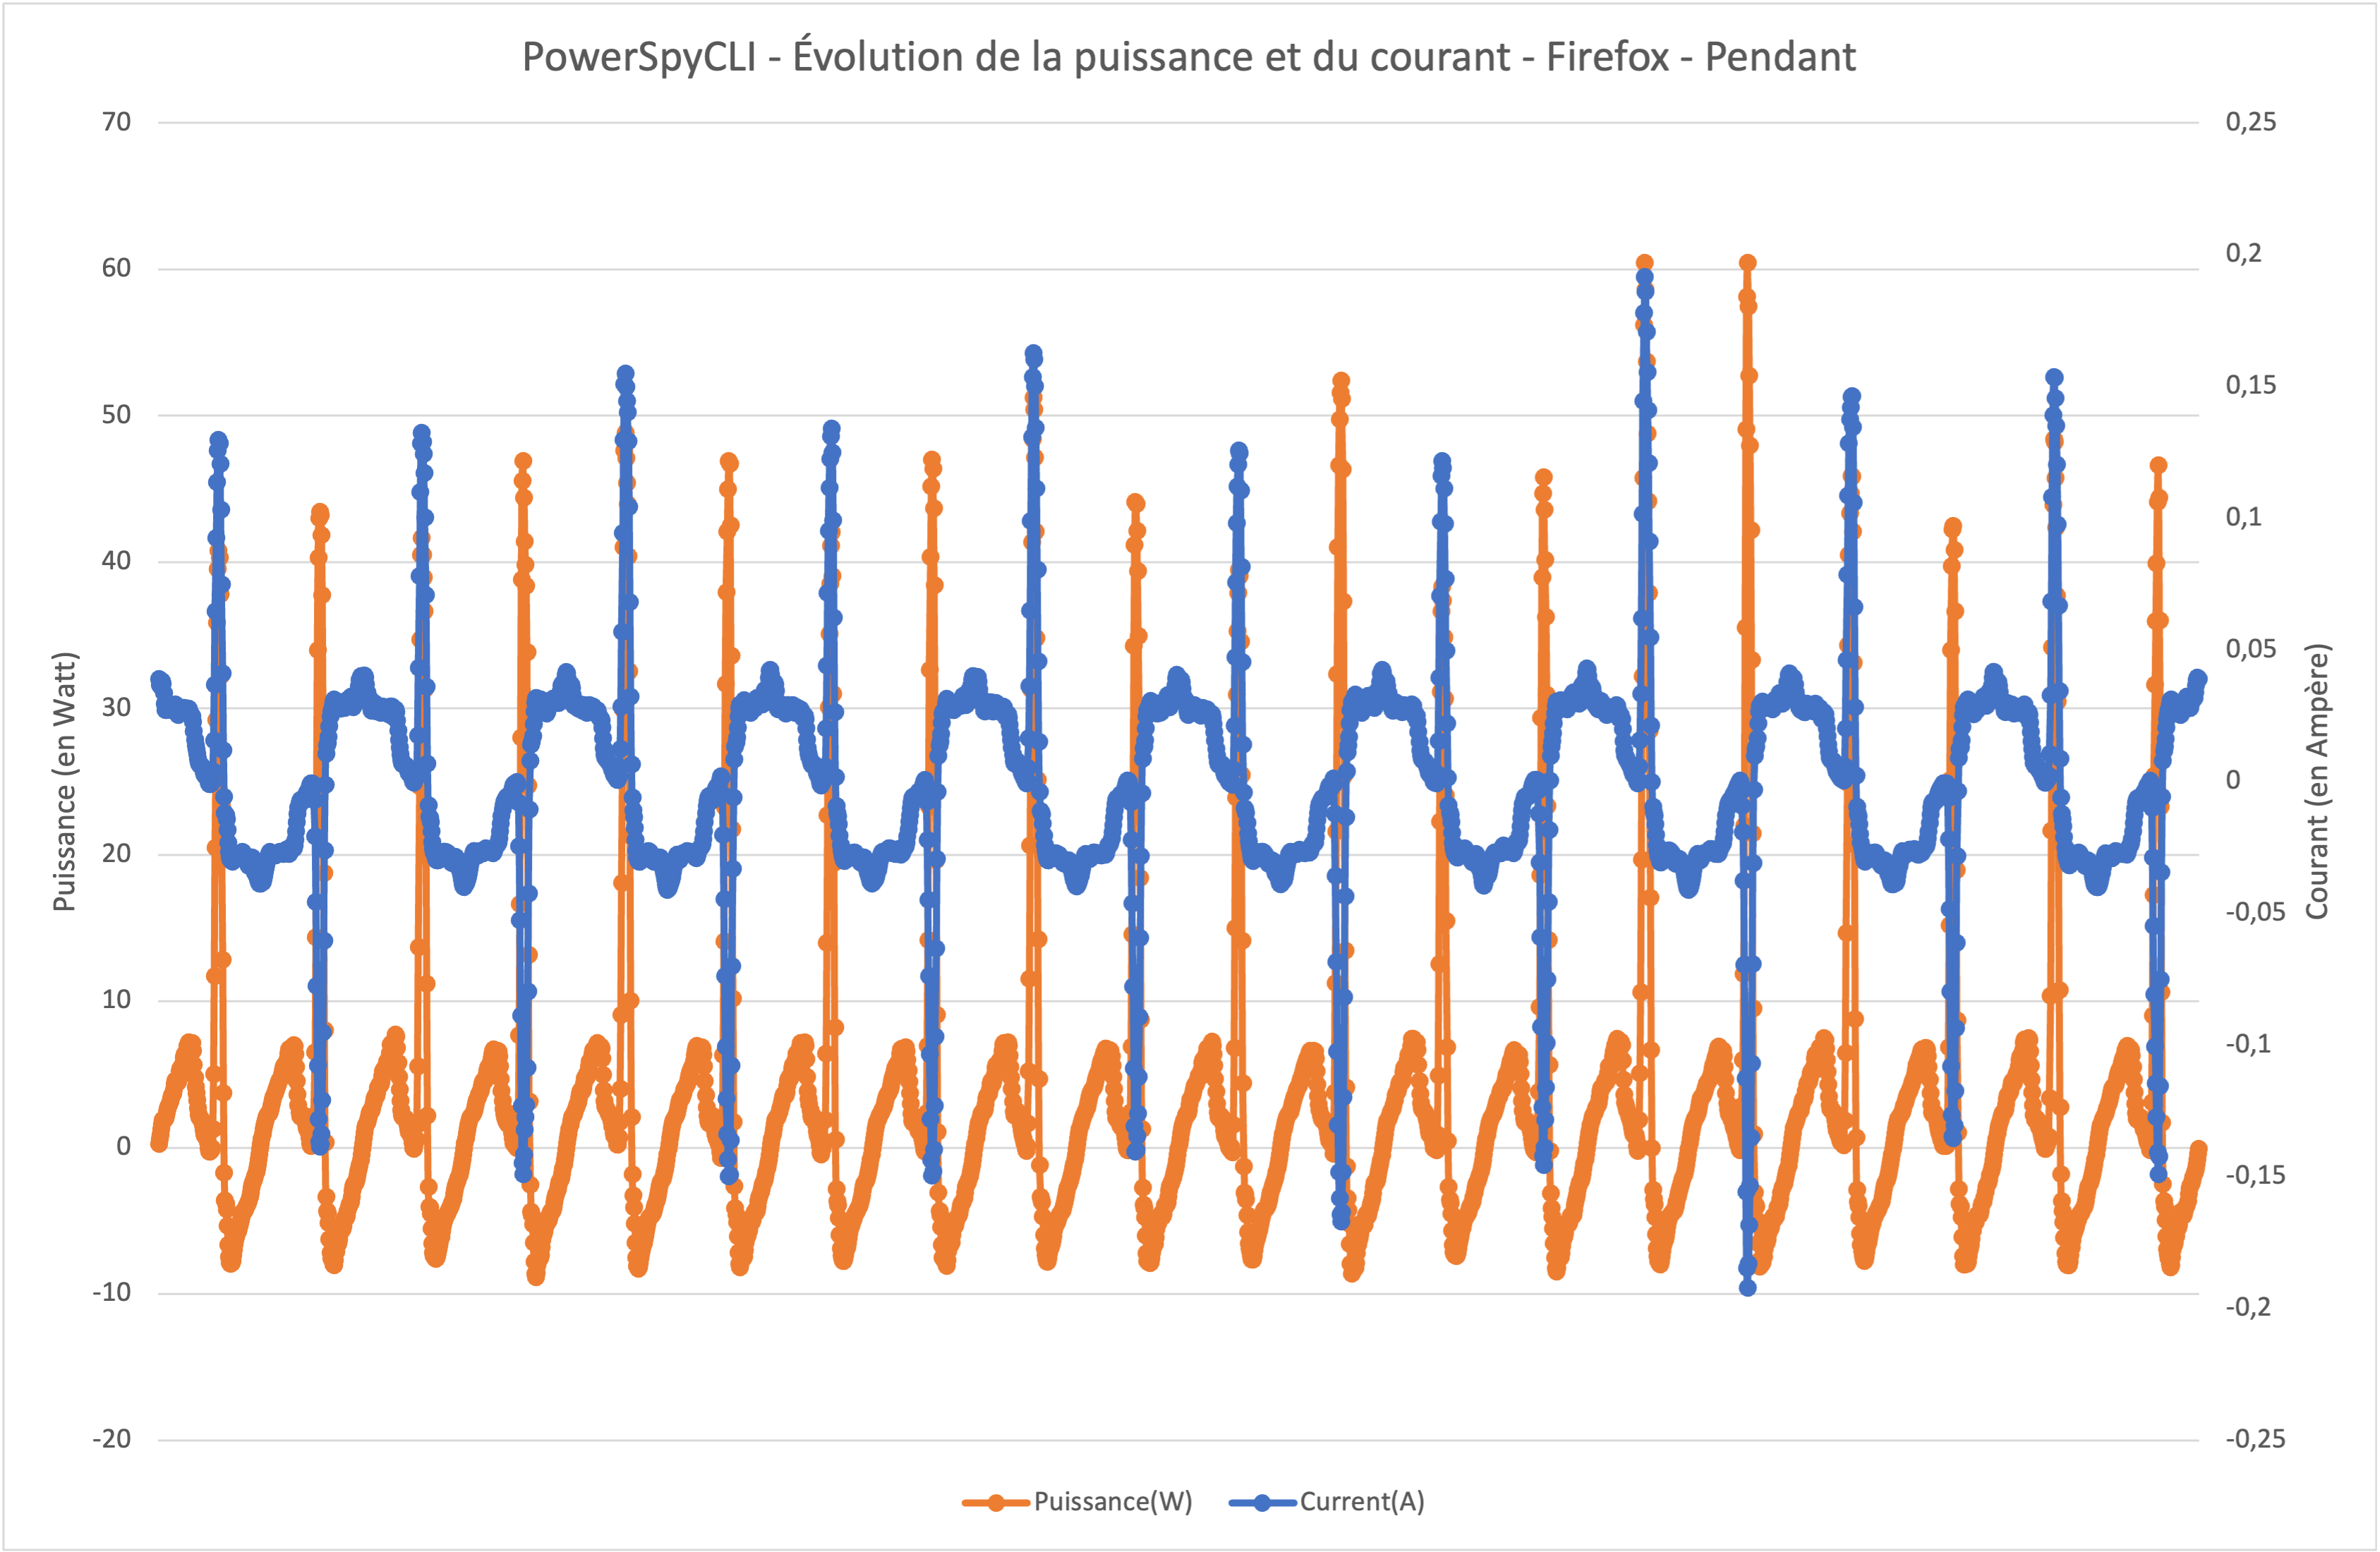
\includegraphics[width=1\linewidth]{res//graph/PowerSpyCLI/Puissance_ff_pendant.png}
    \caption{PowerSpyCLI - Puissance - Firefox - \textit{after}}
    \label{fig:pscli_power_ff_after}
\end{figure}
\begin{figure}[H]
    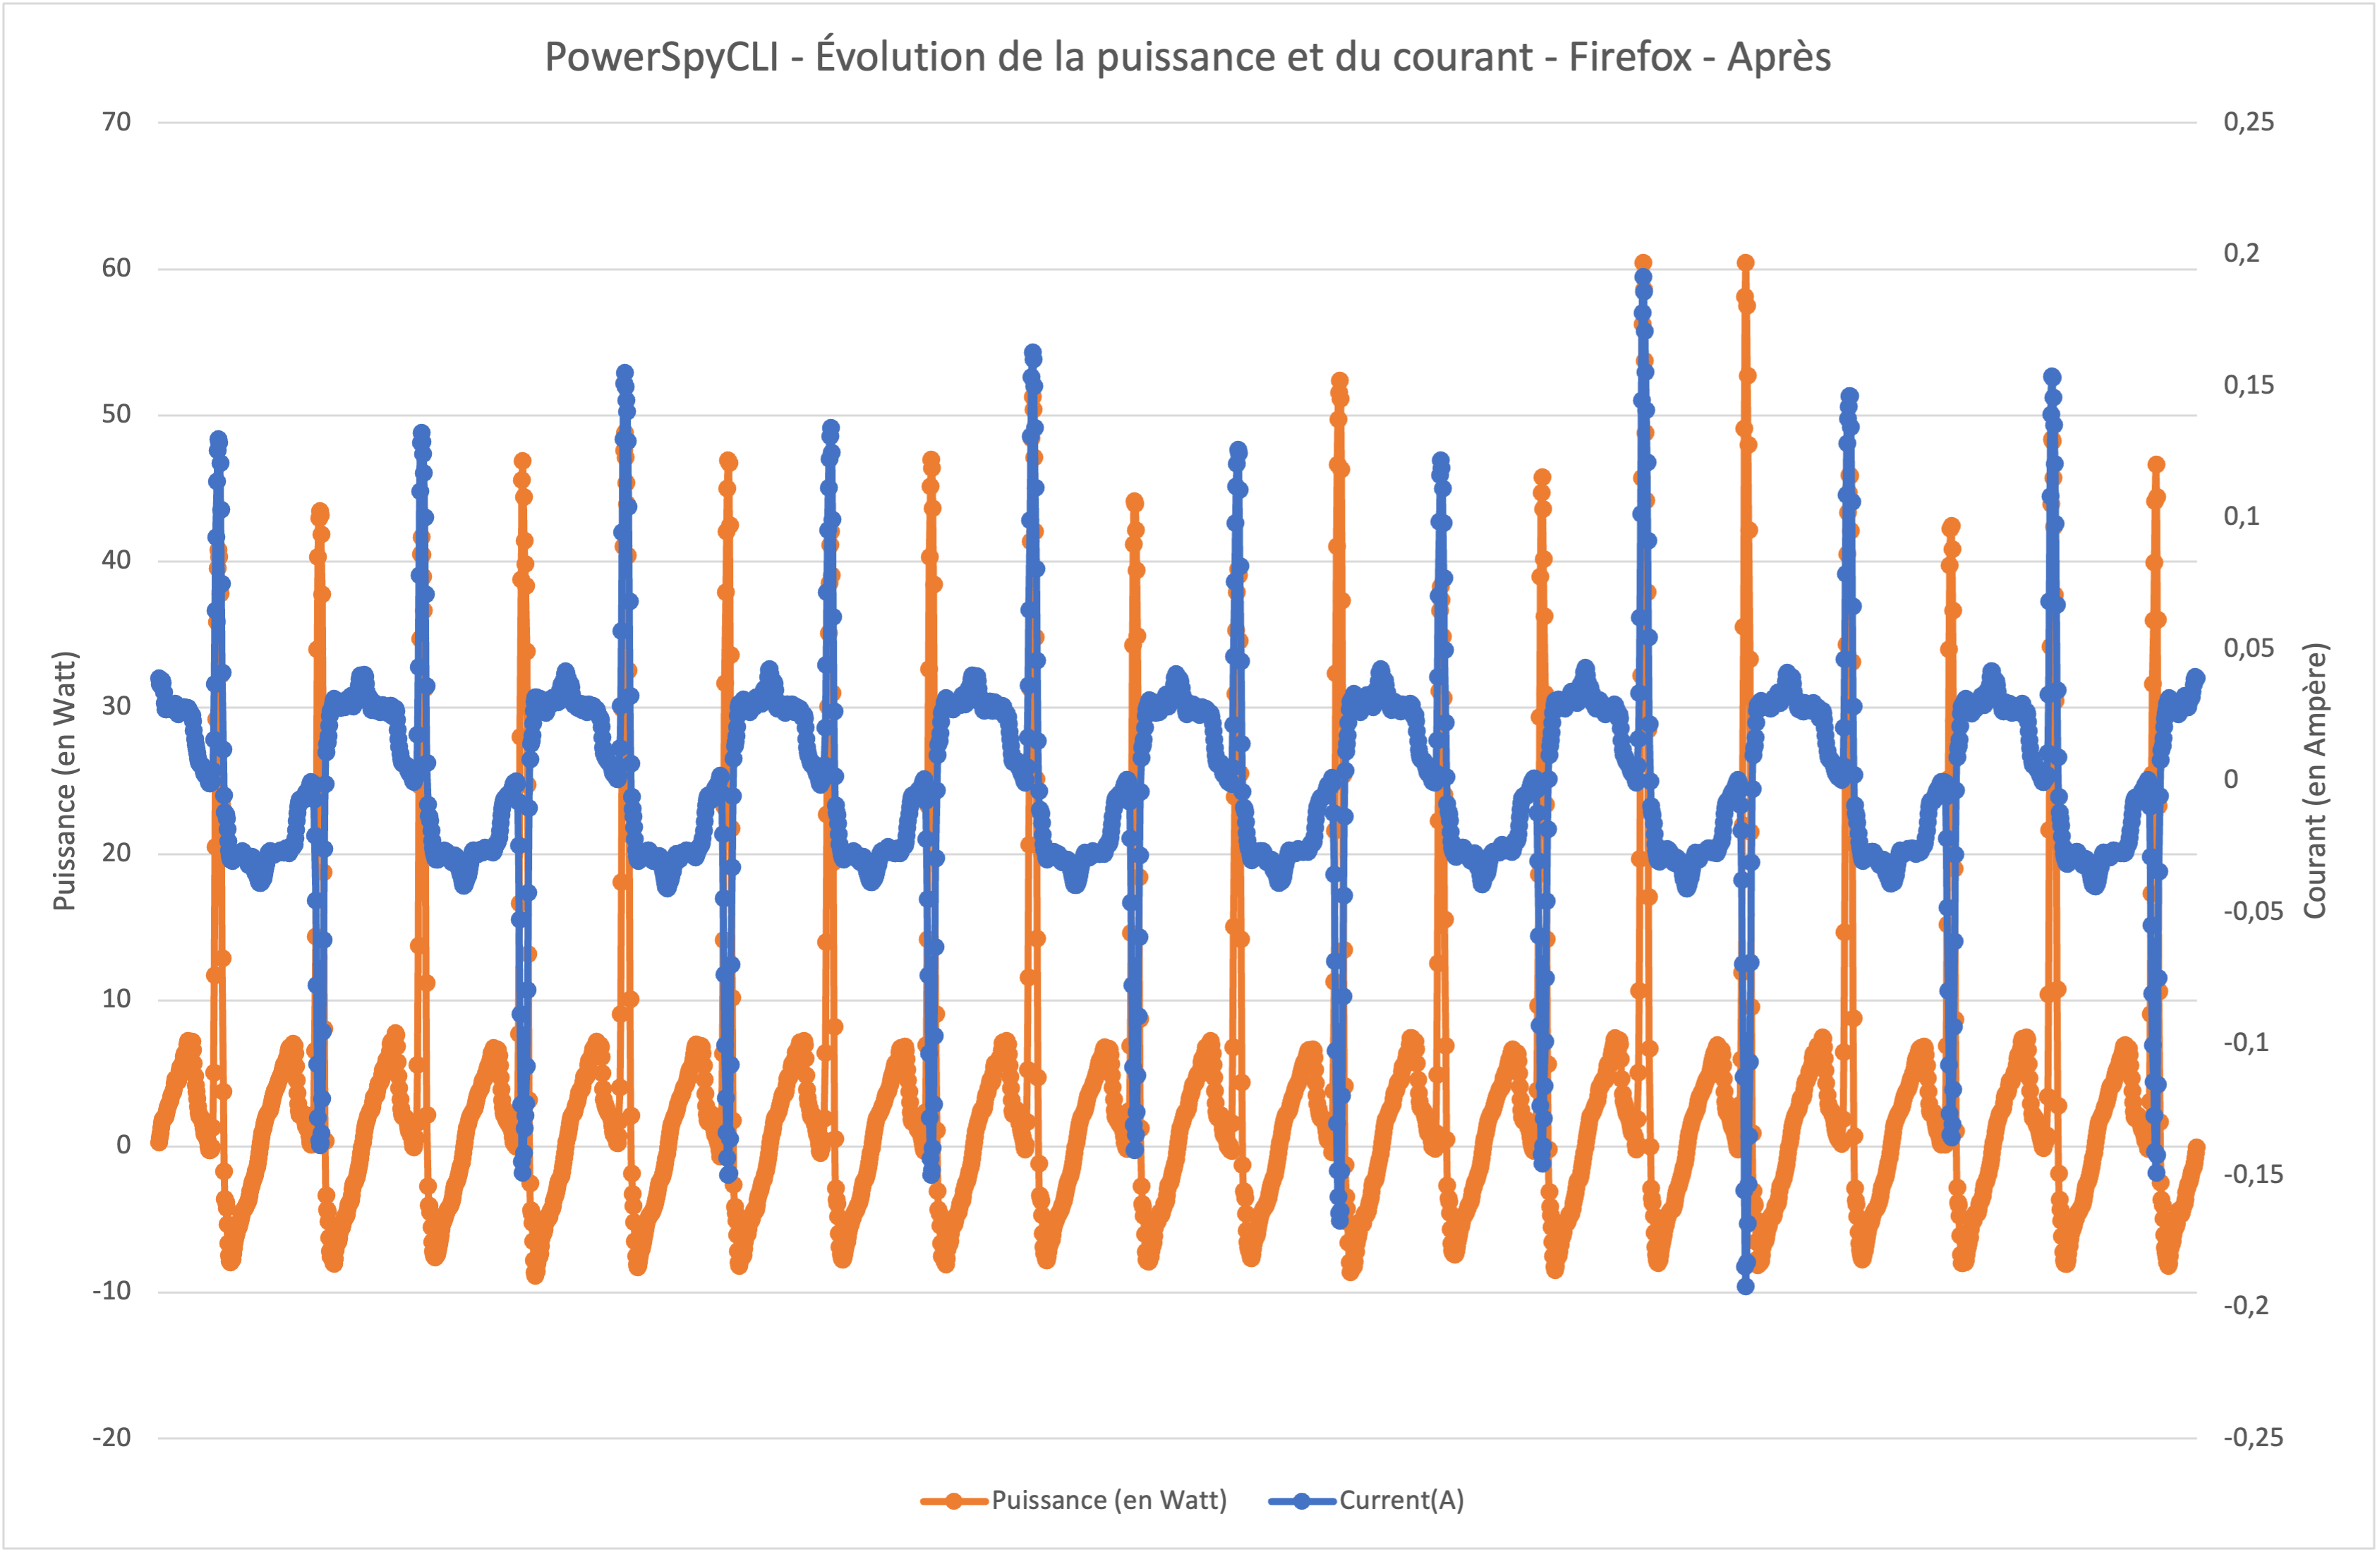
\includegraphics[width=1\linewidth]{res//graph/PowerSpyCLI/Puissance_ff_apres.png}
    \caption{PowerSpyCLI - Puissance - Firefox - \textit{after}}
    \label{fig:pscli_power_ff_after}
\end{figure}
De part les résultats obtenus précédement, nous nous attendions à un résultat similaire lors du calcul de la puissance pour chaque étape de l'expérience. 

\subsubsection{PowerSpy2}
PowerSpy2 est très similaire à PowerSpyCLI. Il s'agit en réalité d'une version avec une interface graphique. Les données sorties par le logiciel sont les même que pour la version en ligne de commande, nous avons donc: 
\begin{itemize}
    \item Id (Fonctionne comme un timestamp)
    \item Courant (A)
    \item Voltage (V)
\end{itemize}

Nous pouvons de nouveau calculer la puissance grâce à la formule \ref{eq:puissance}. Voici nos résultats obtenus. Chaque étape de l'expérience a 2 graphiques différents comme précédemment. Une pour la comparaison entre le voltage et le courant et une autre pour la différence entre la puissance et le courant.
Nous allons directement afficher nos 6 différents graphiques, puis nous les commenterons ensemble en conclusion ci-dessous. Les trois premiers représentent l'évolution du courant et du voltage sur Firefox avant, pendant et après la lecture de la vidéo.
Puis, après avoir calculé la puissance, nous avons graphé l'évolution du courant et de la puissance par rapport au temps. 

\paragraph{
\textbf{Courant}}
\begin{figure}[H]
    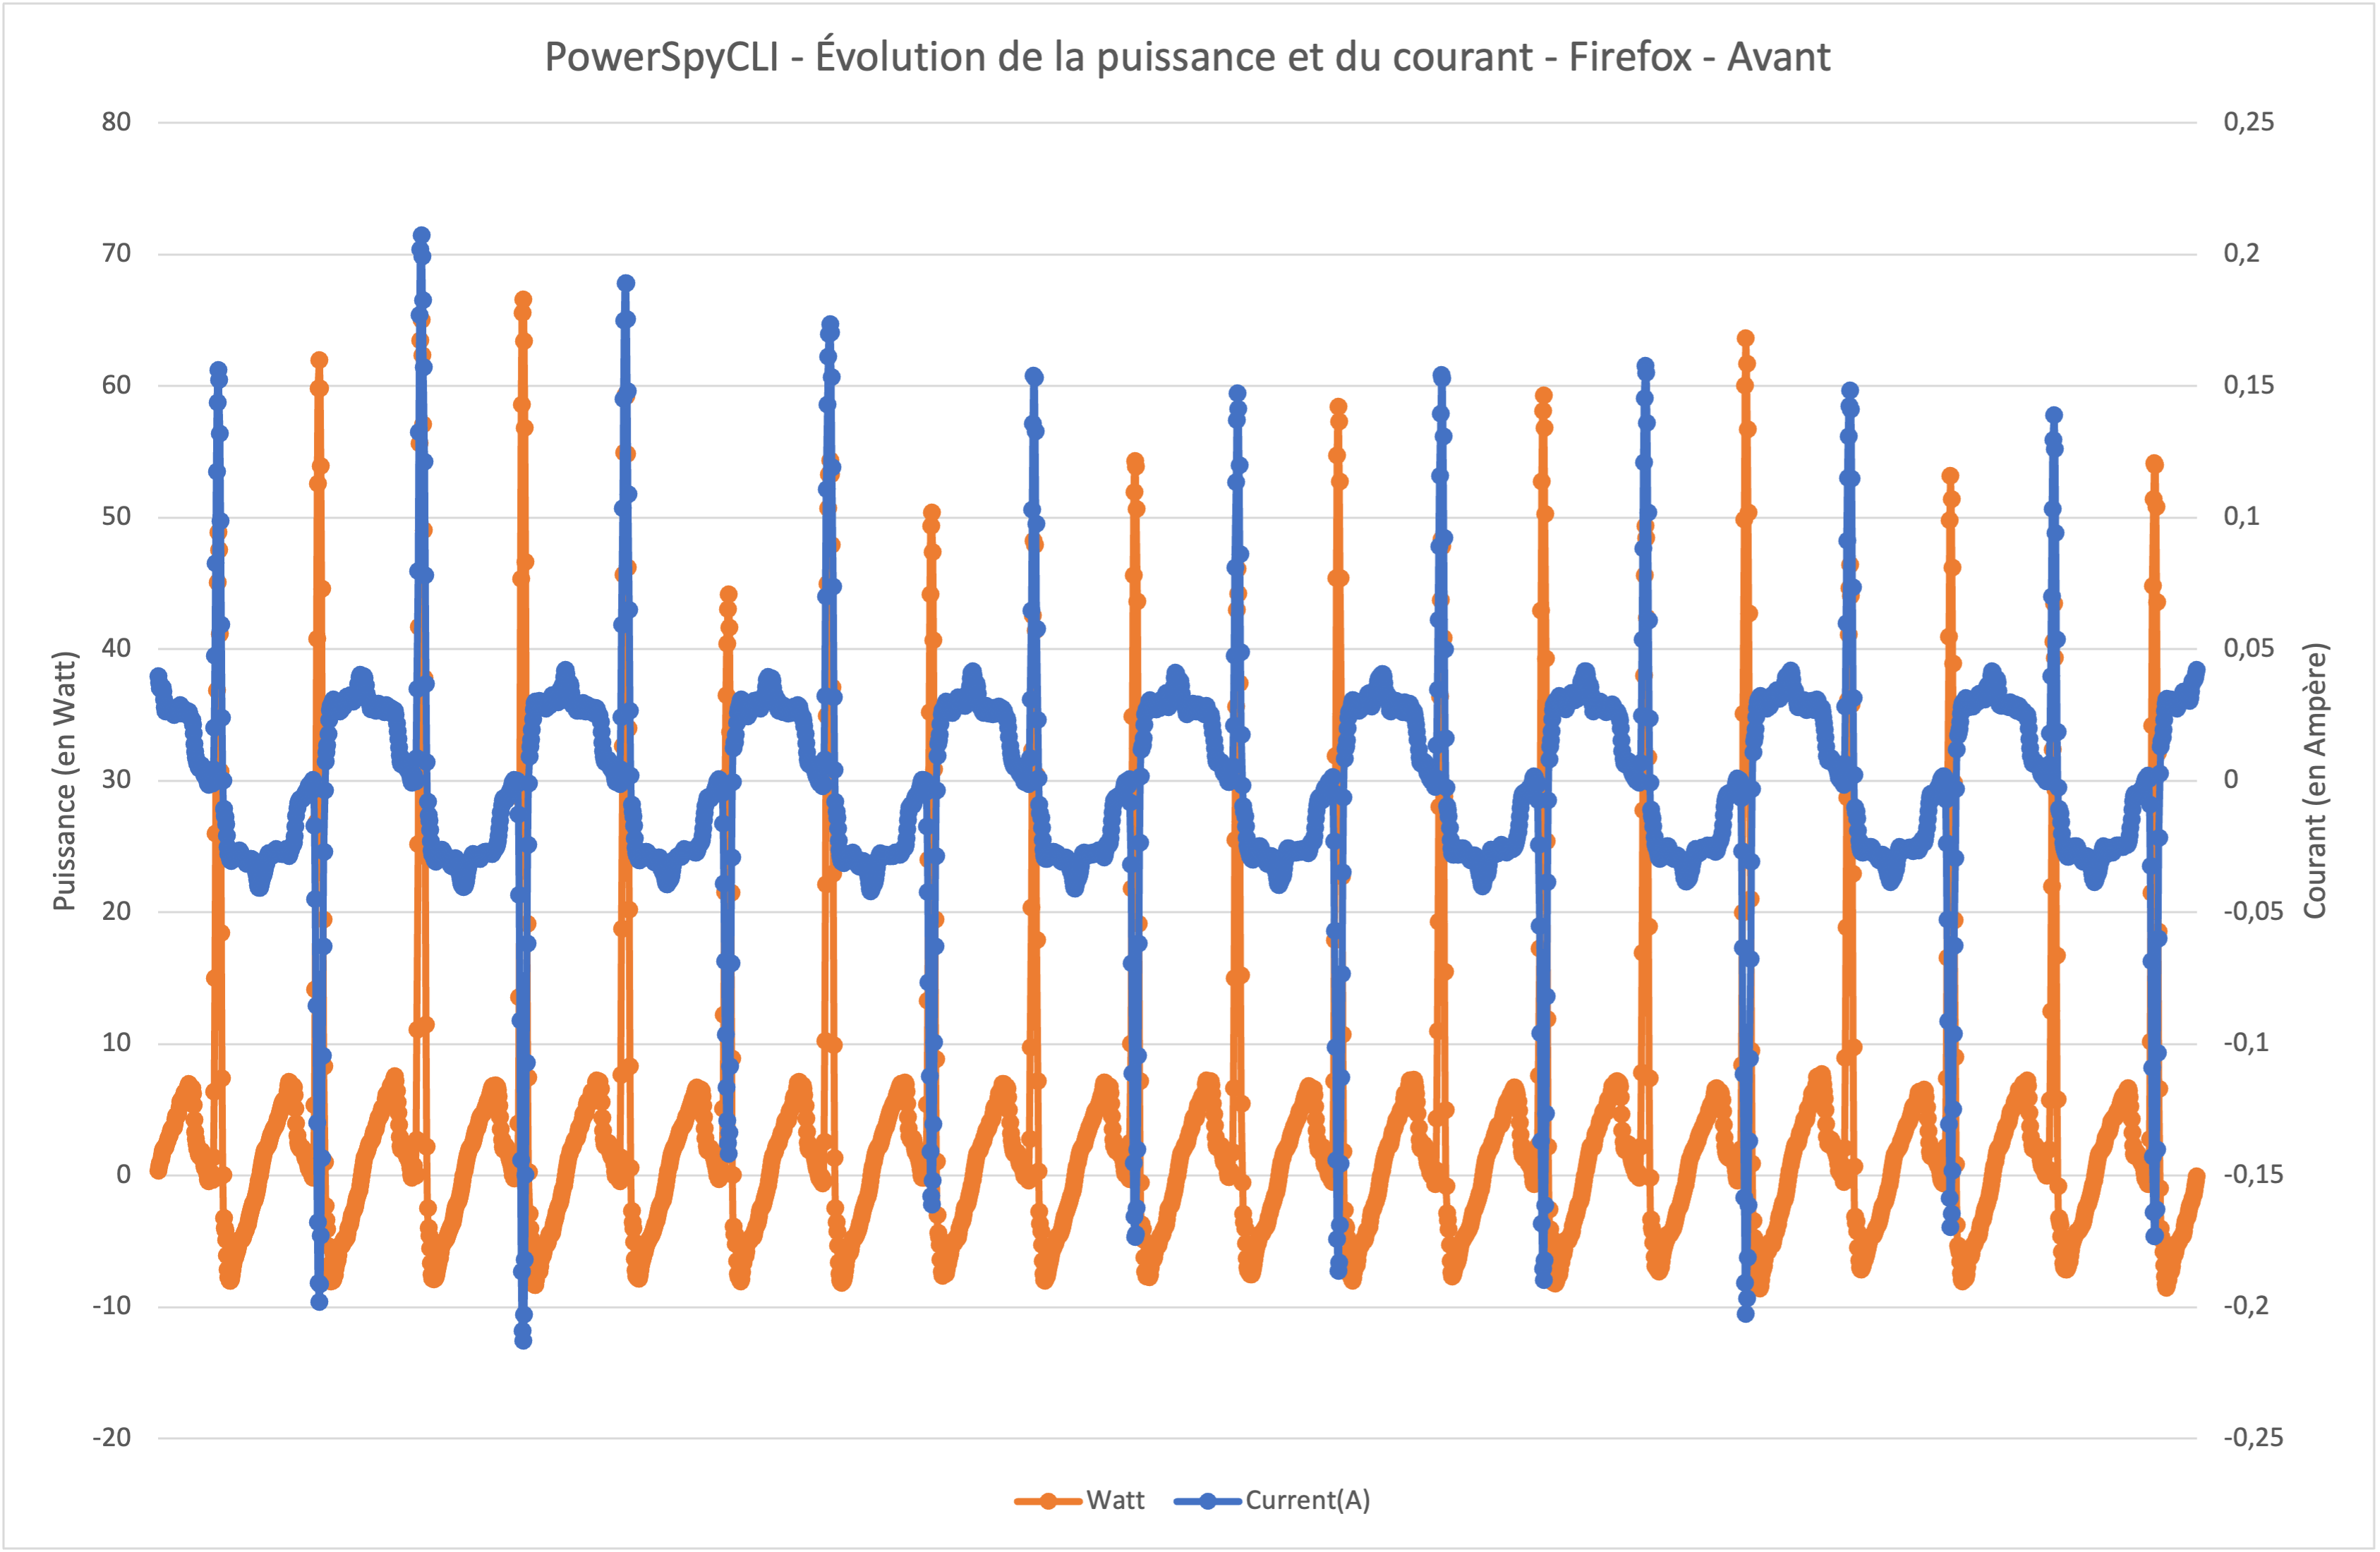
\includegraphics[width=1\linewidth]{res//graph/PowerSpyCLI/Puissance_ff_avant.png}
    \caption{PowerSpyCLI - Puissance - Firefox - \textit{avant}}
    \label{fig:pscli_power_ff_after}
\end{figure}
\begin{figure}[H]
    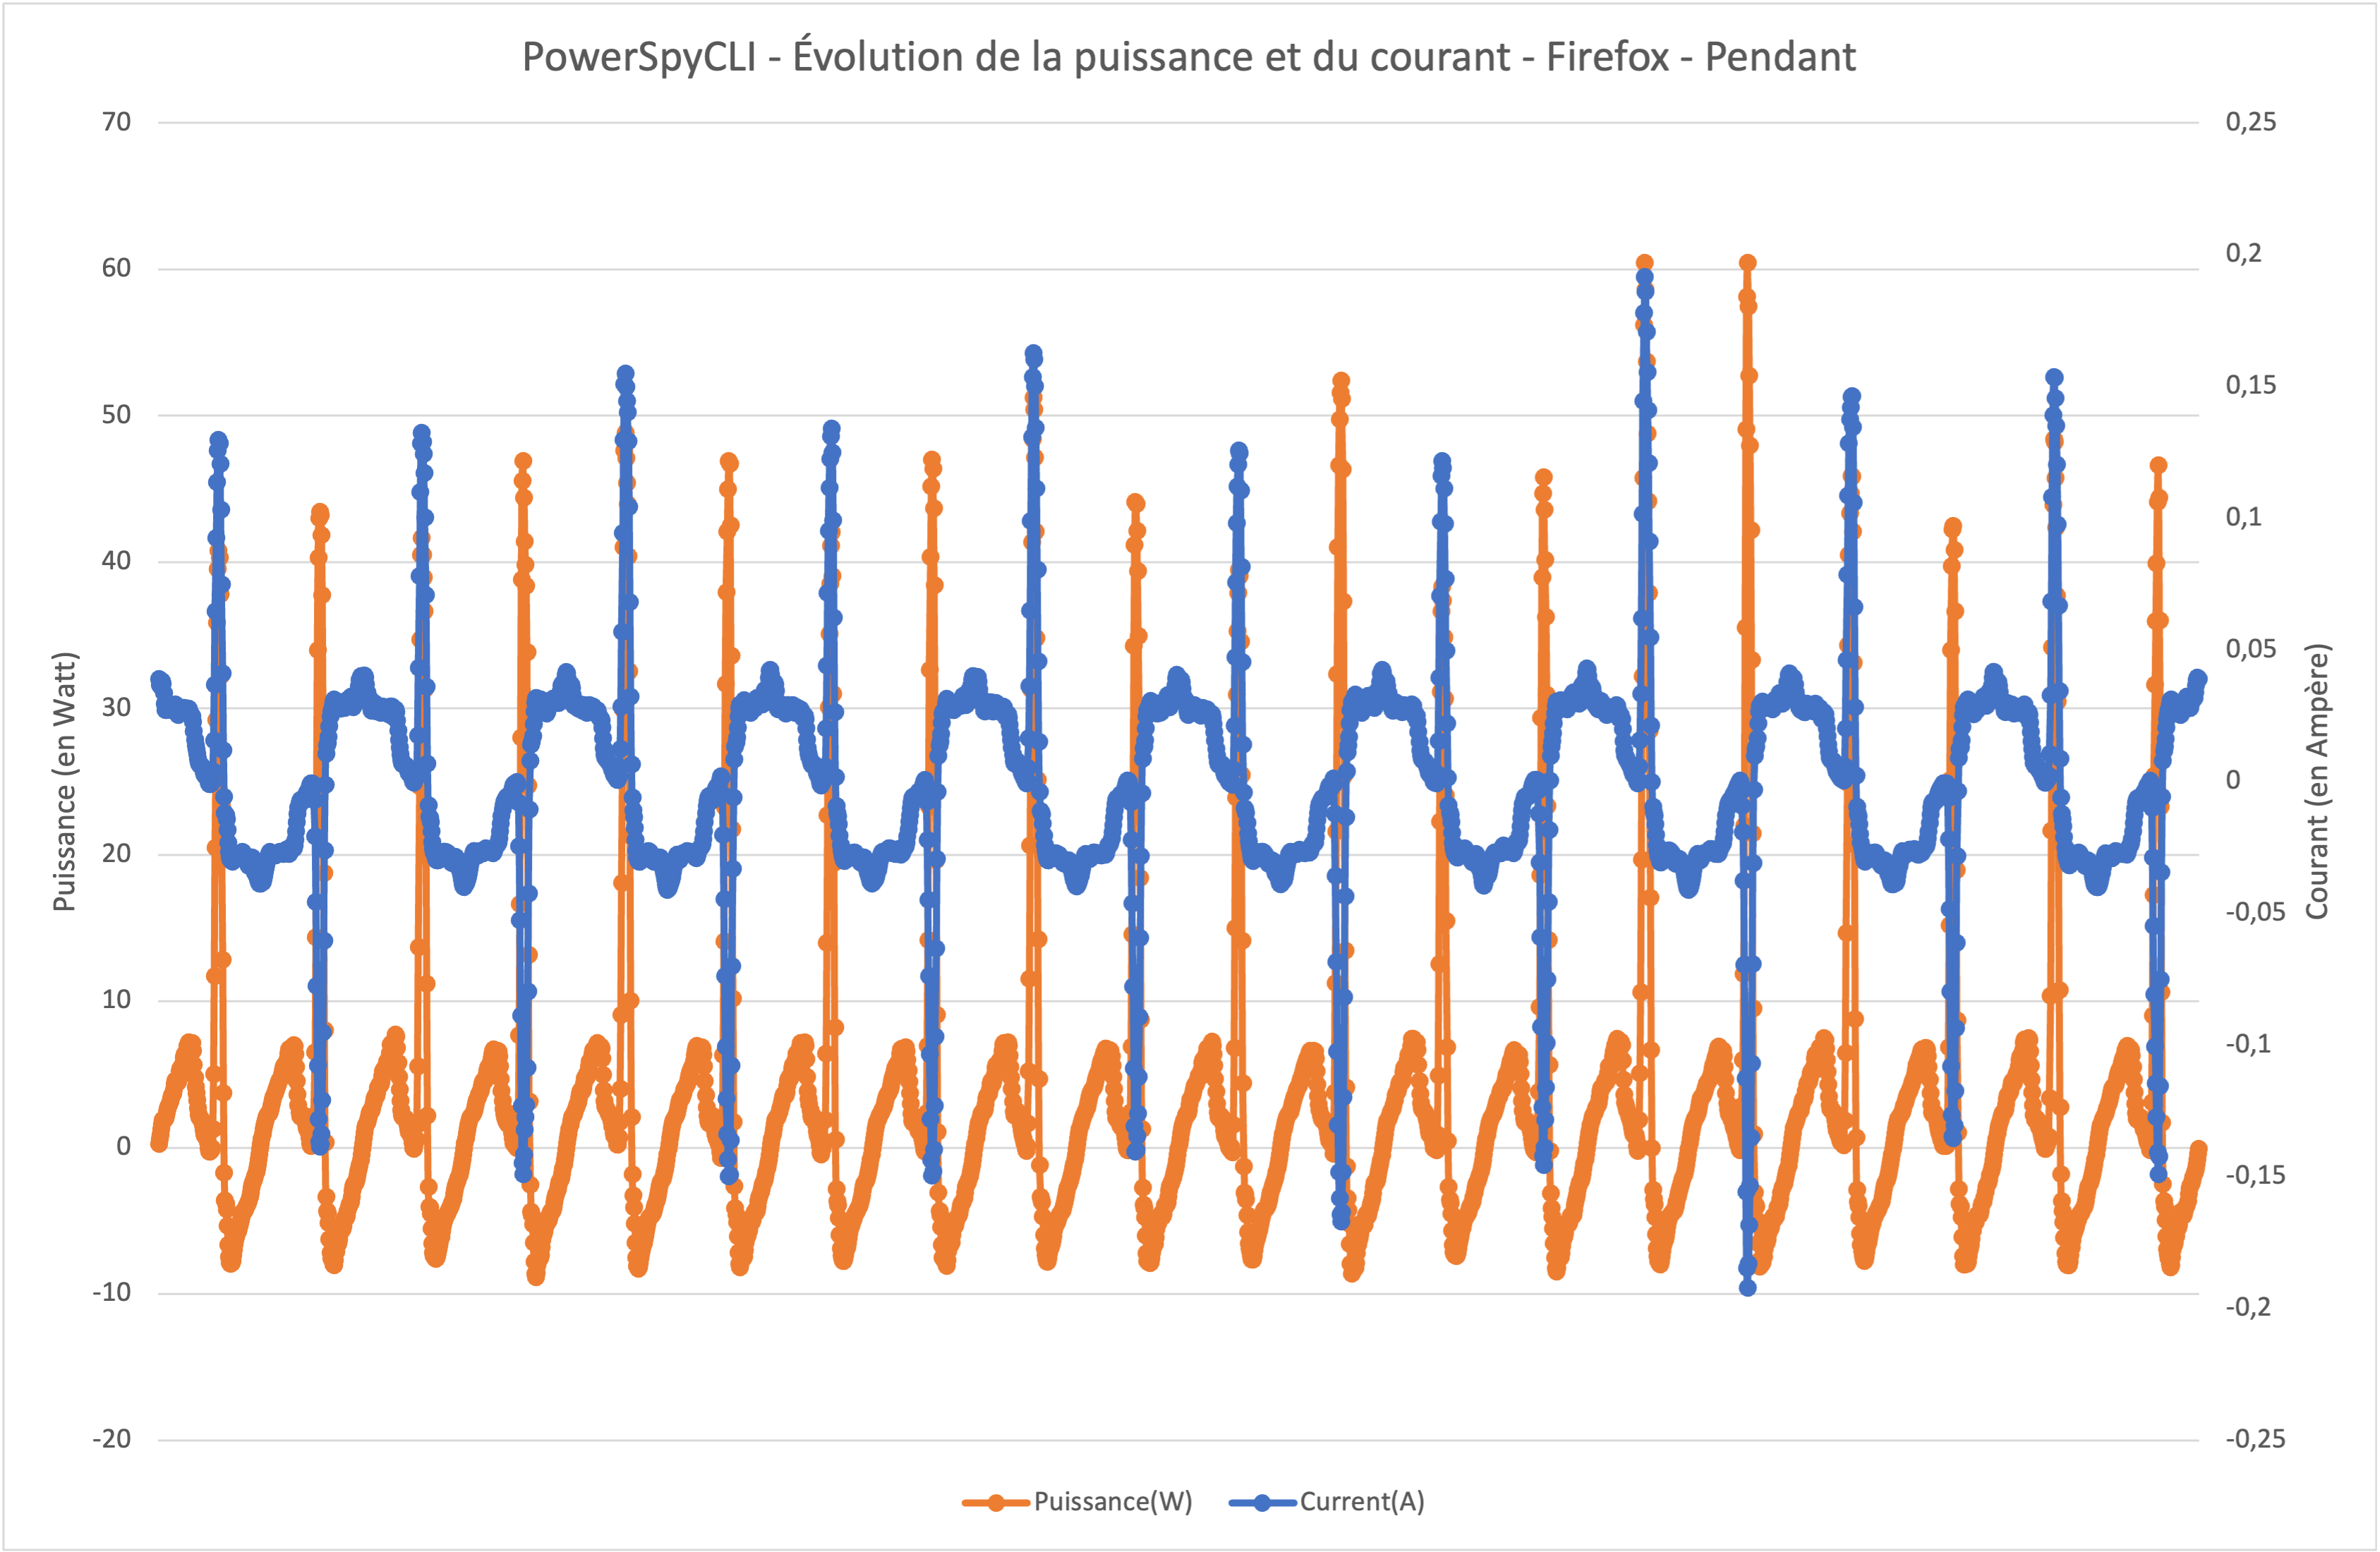
\includegraphics[width=1\linewidth]{res//graph/PowerSpyCLI/Puissance_ff_pendant.png}
    \caption{PowerSpyCLI - Puissance - Firefox - \textit{during}}
    \label{fig:pscli_power_ff_after}
\end{figure}
\begin{figure}[H]
    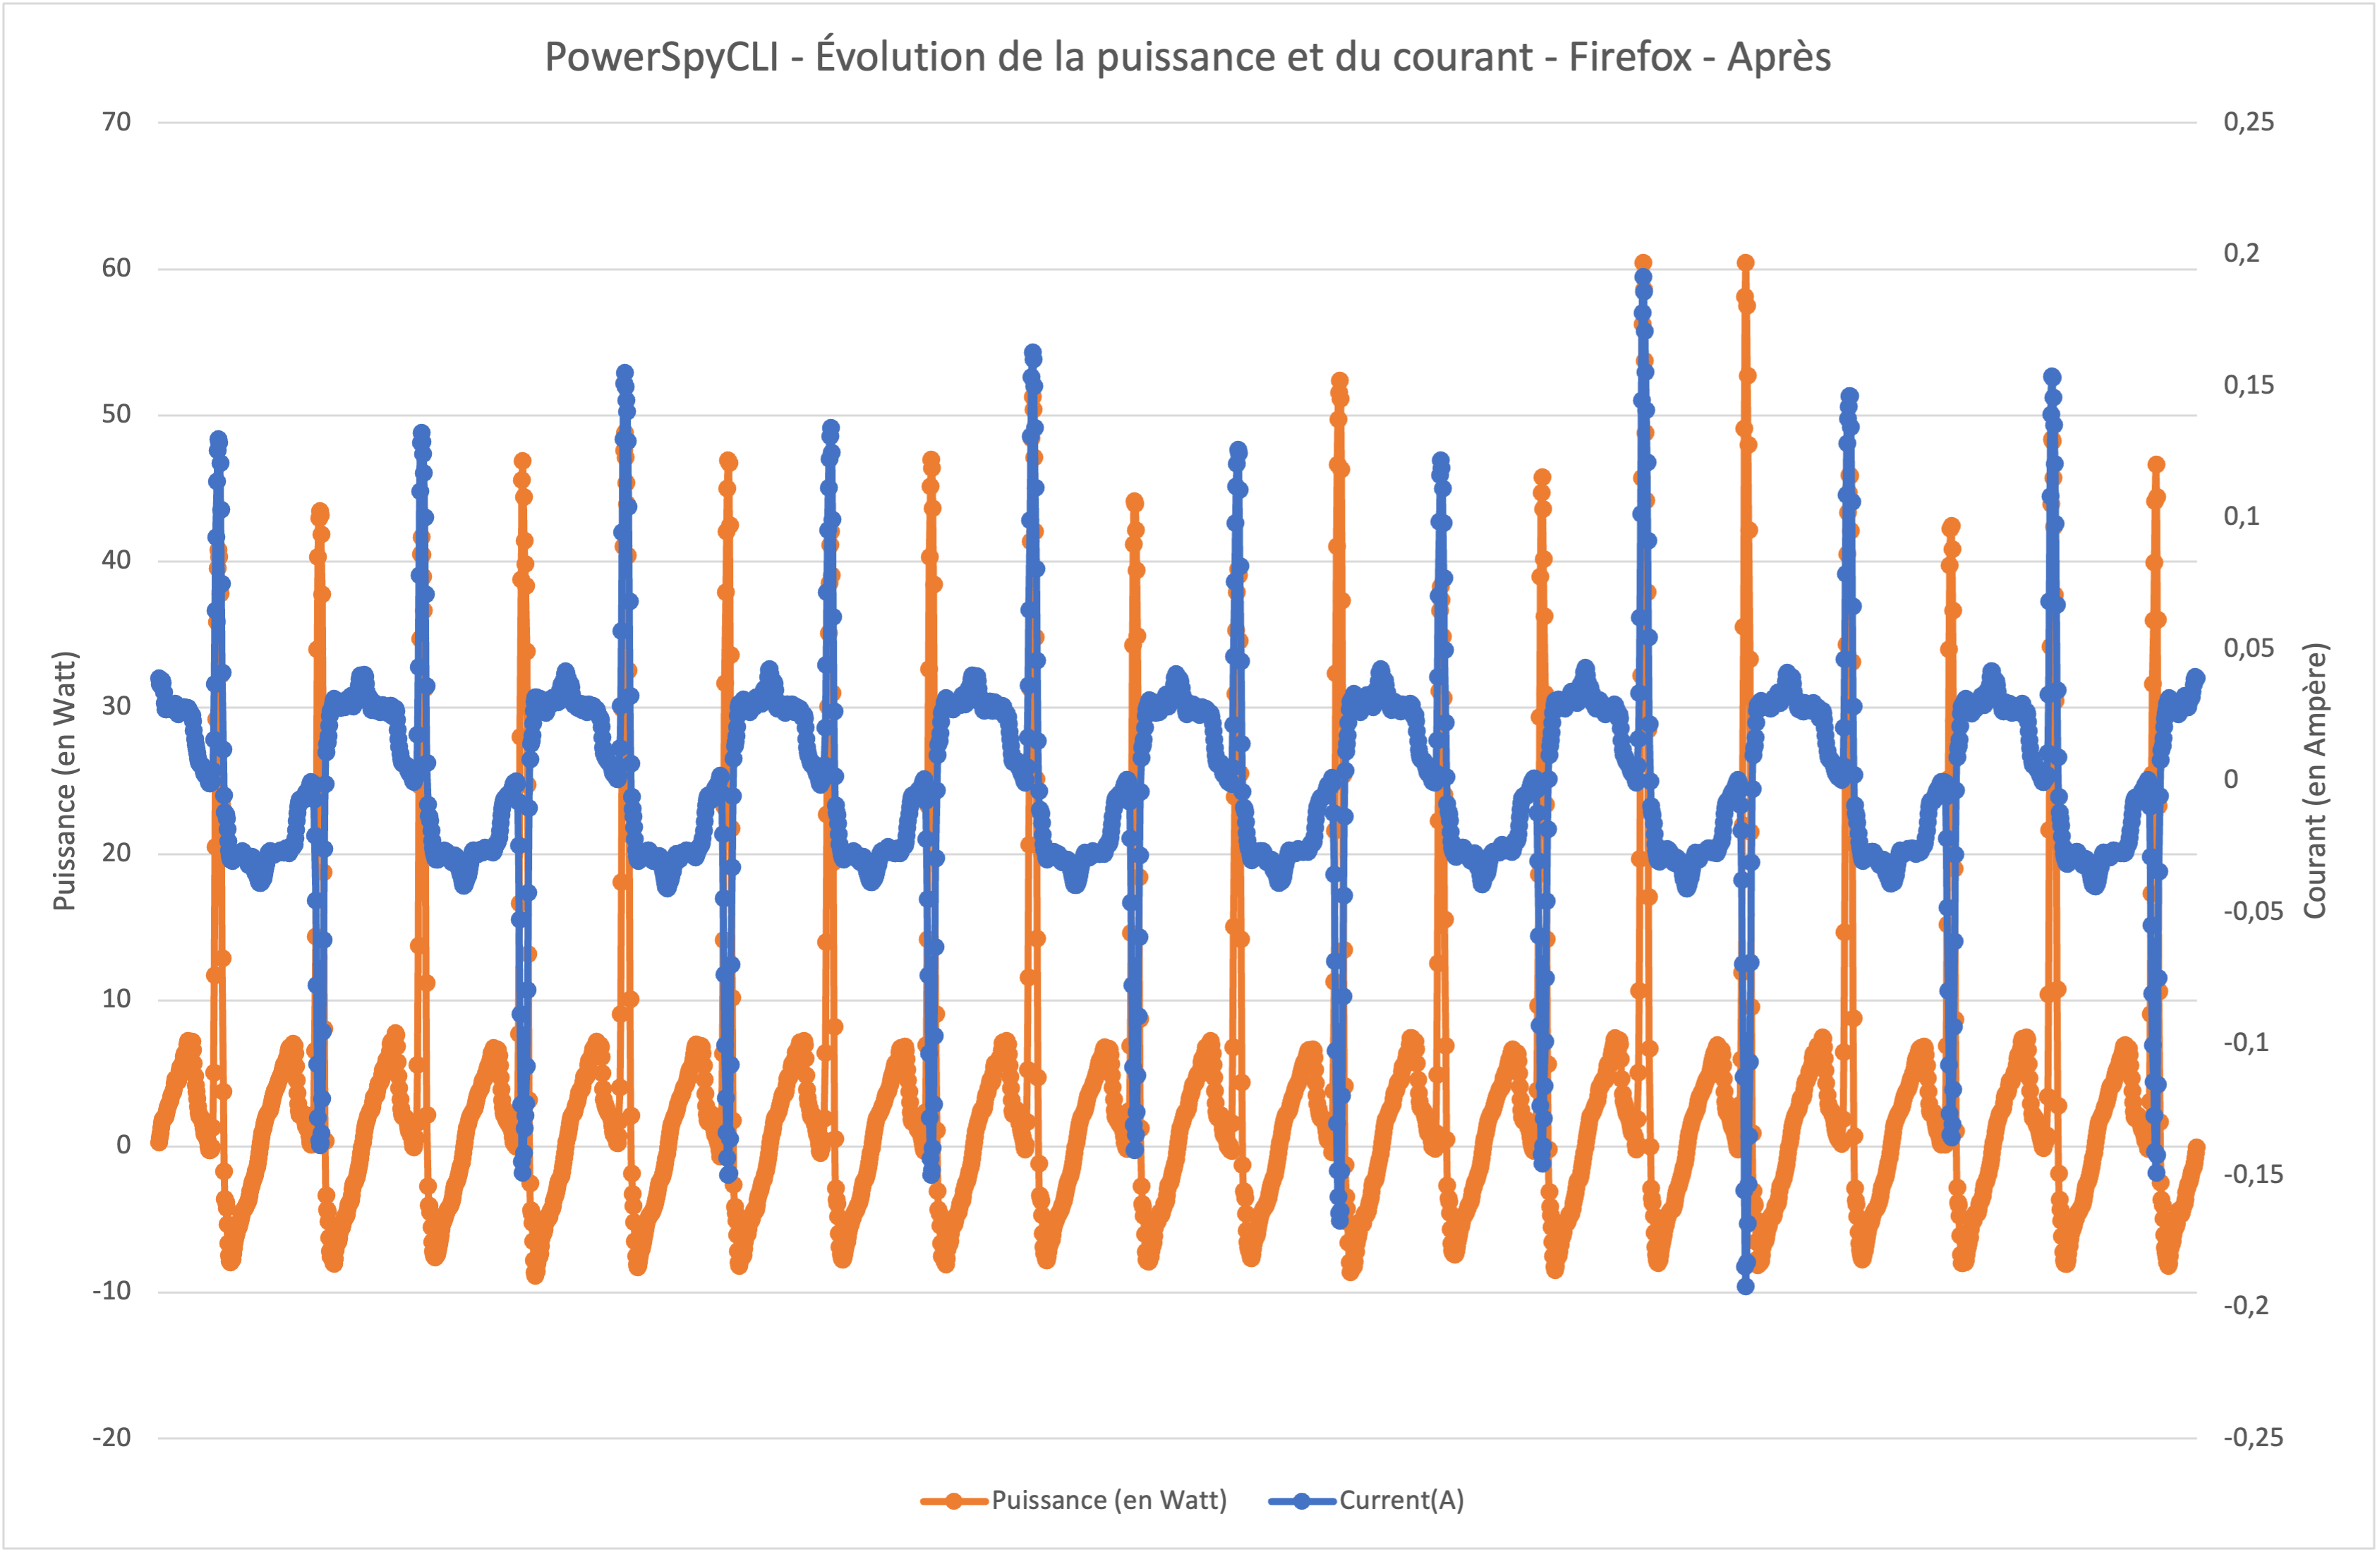
\includegraphics[width=1\linewidth]{res//graph/PowerSpyCLI/Puissance_ff_apres.png}
    \caption{PowerSpyCLI - Puissance - Firefox - \textit{after}}
    \label{fig:pscli_power_ff_after}
\end{figure}


\paragraph{
\textbf{Puissance}}
\begin{figure}[H]
    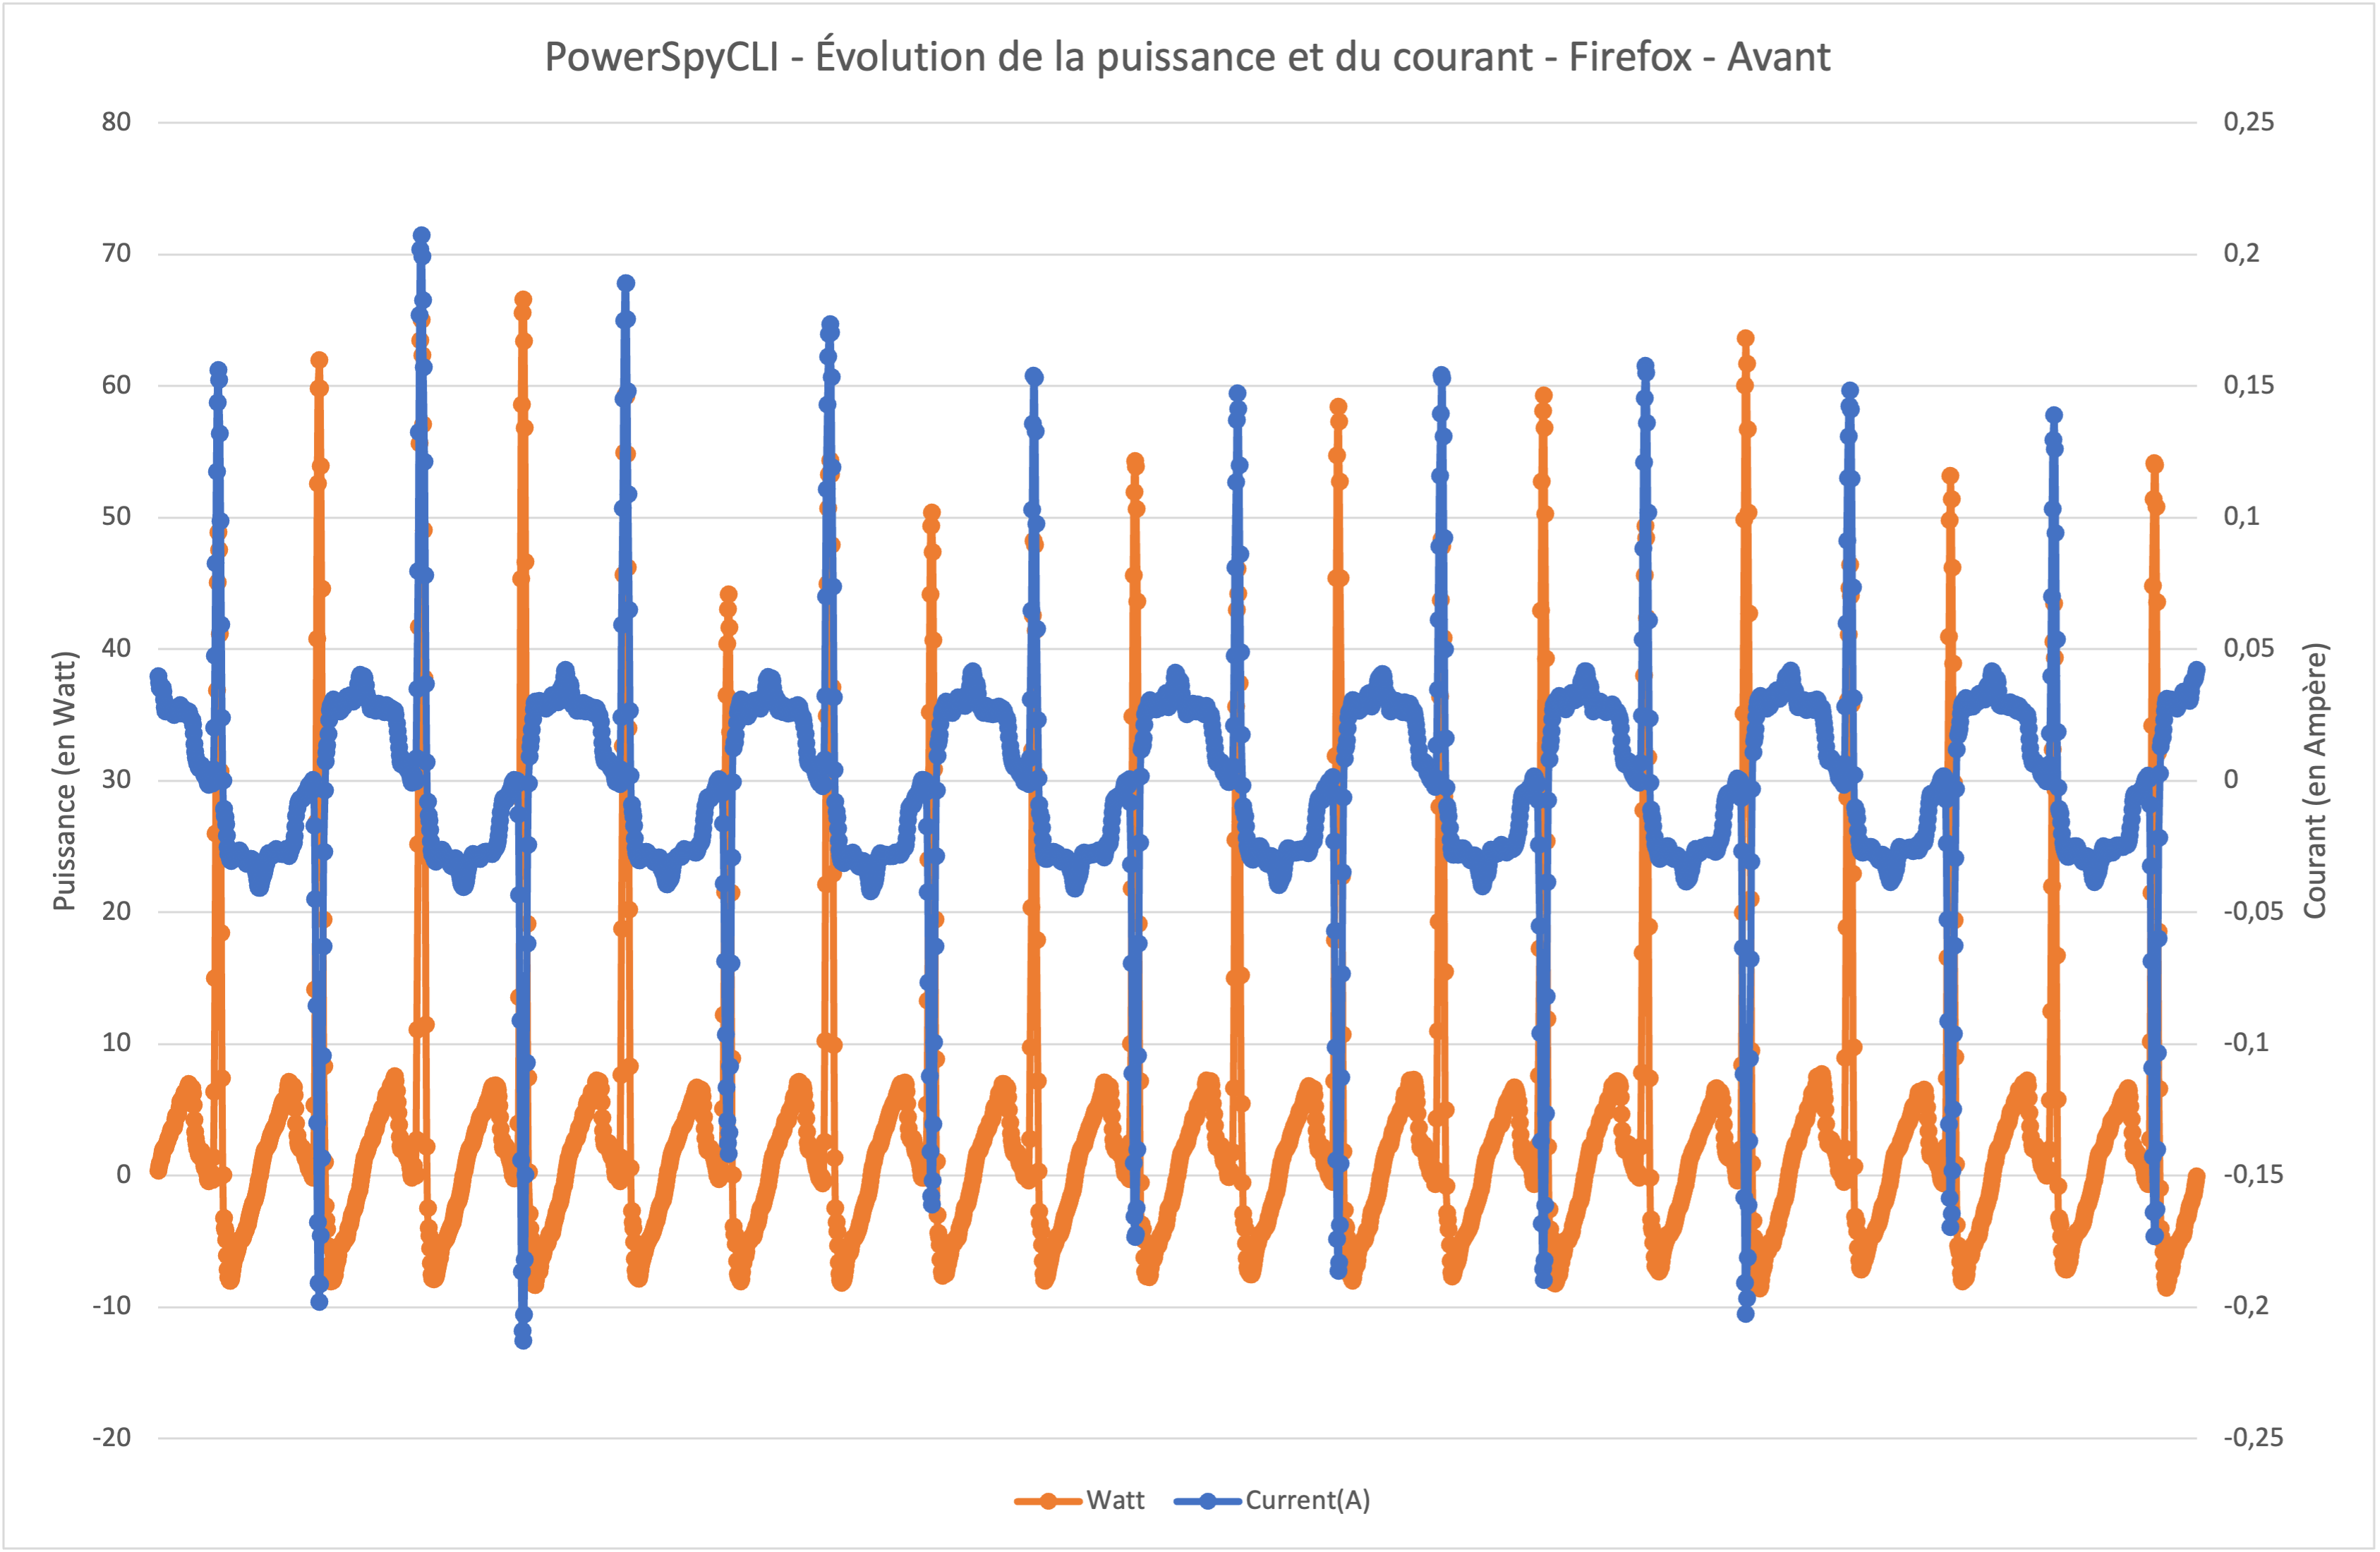
\includegraphics[width=1\linewidth]{res//graph/PowerSpyCLI/Puissance_ff_avant.png}
    \caption{PowerSpyCLI - Puissance - Firefox - \textit{avant}}
    \label{fig:pscli_power_ff_after}
\end{figure}
\begin{figure}[H]
    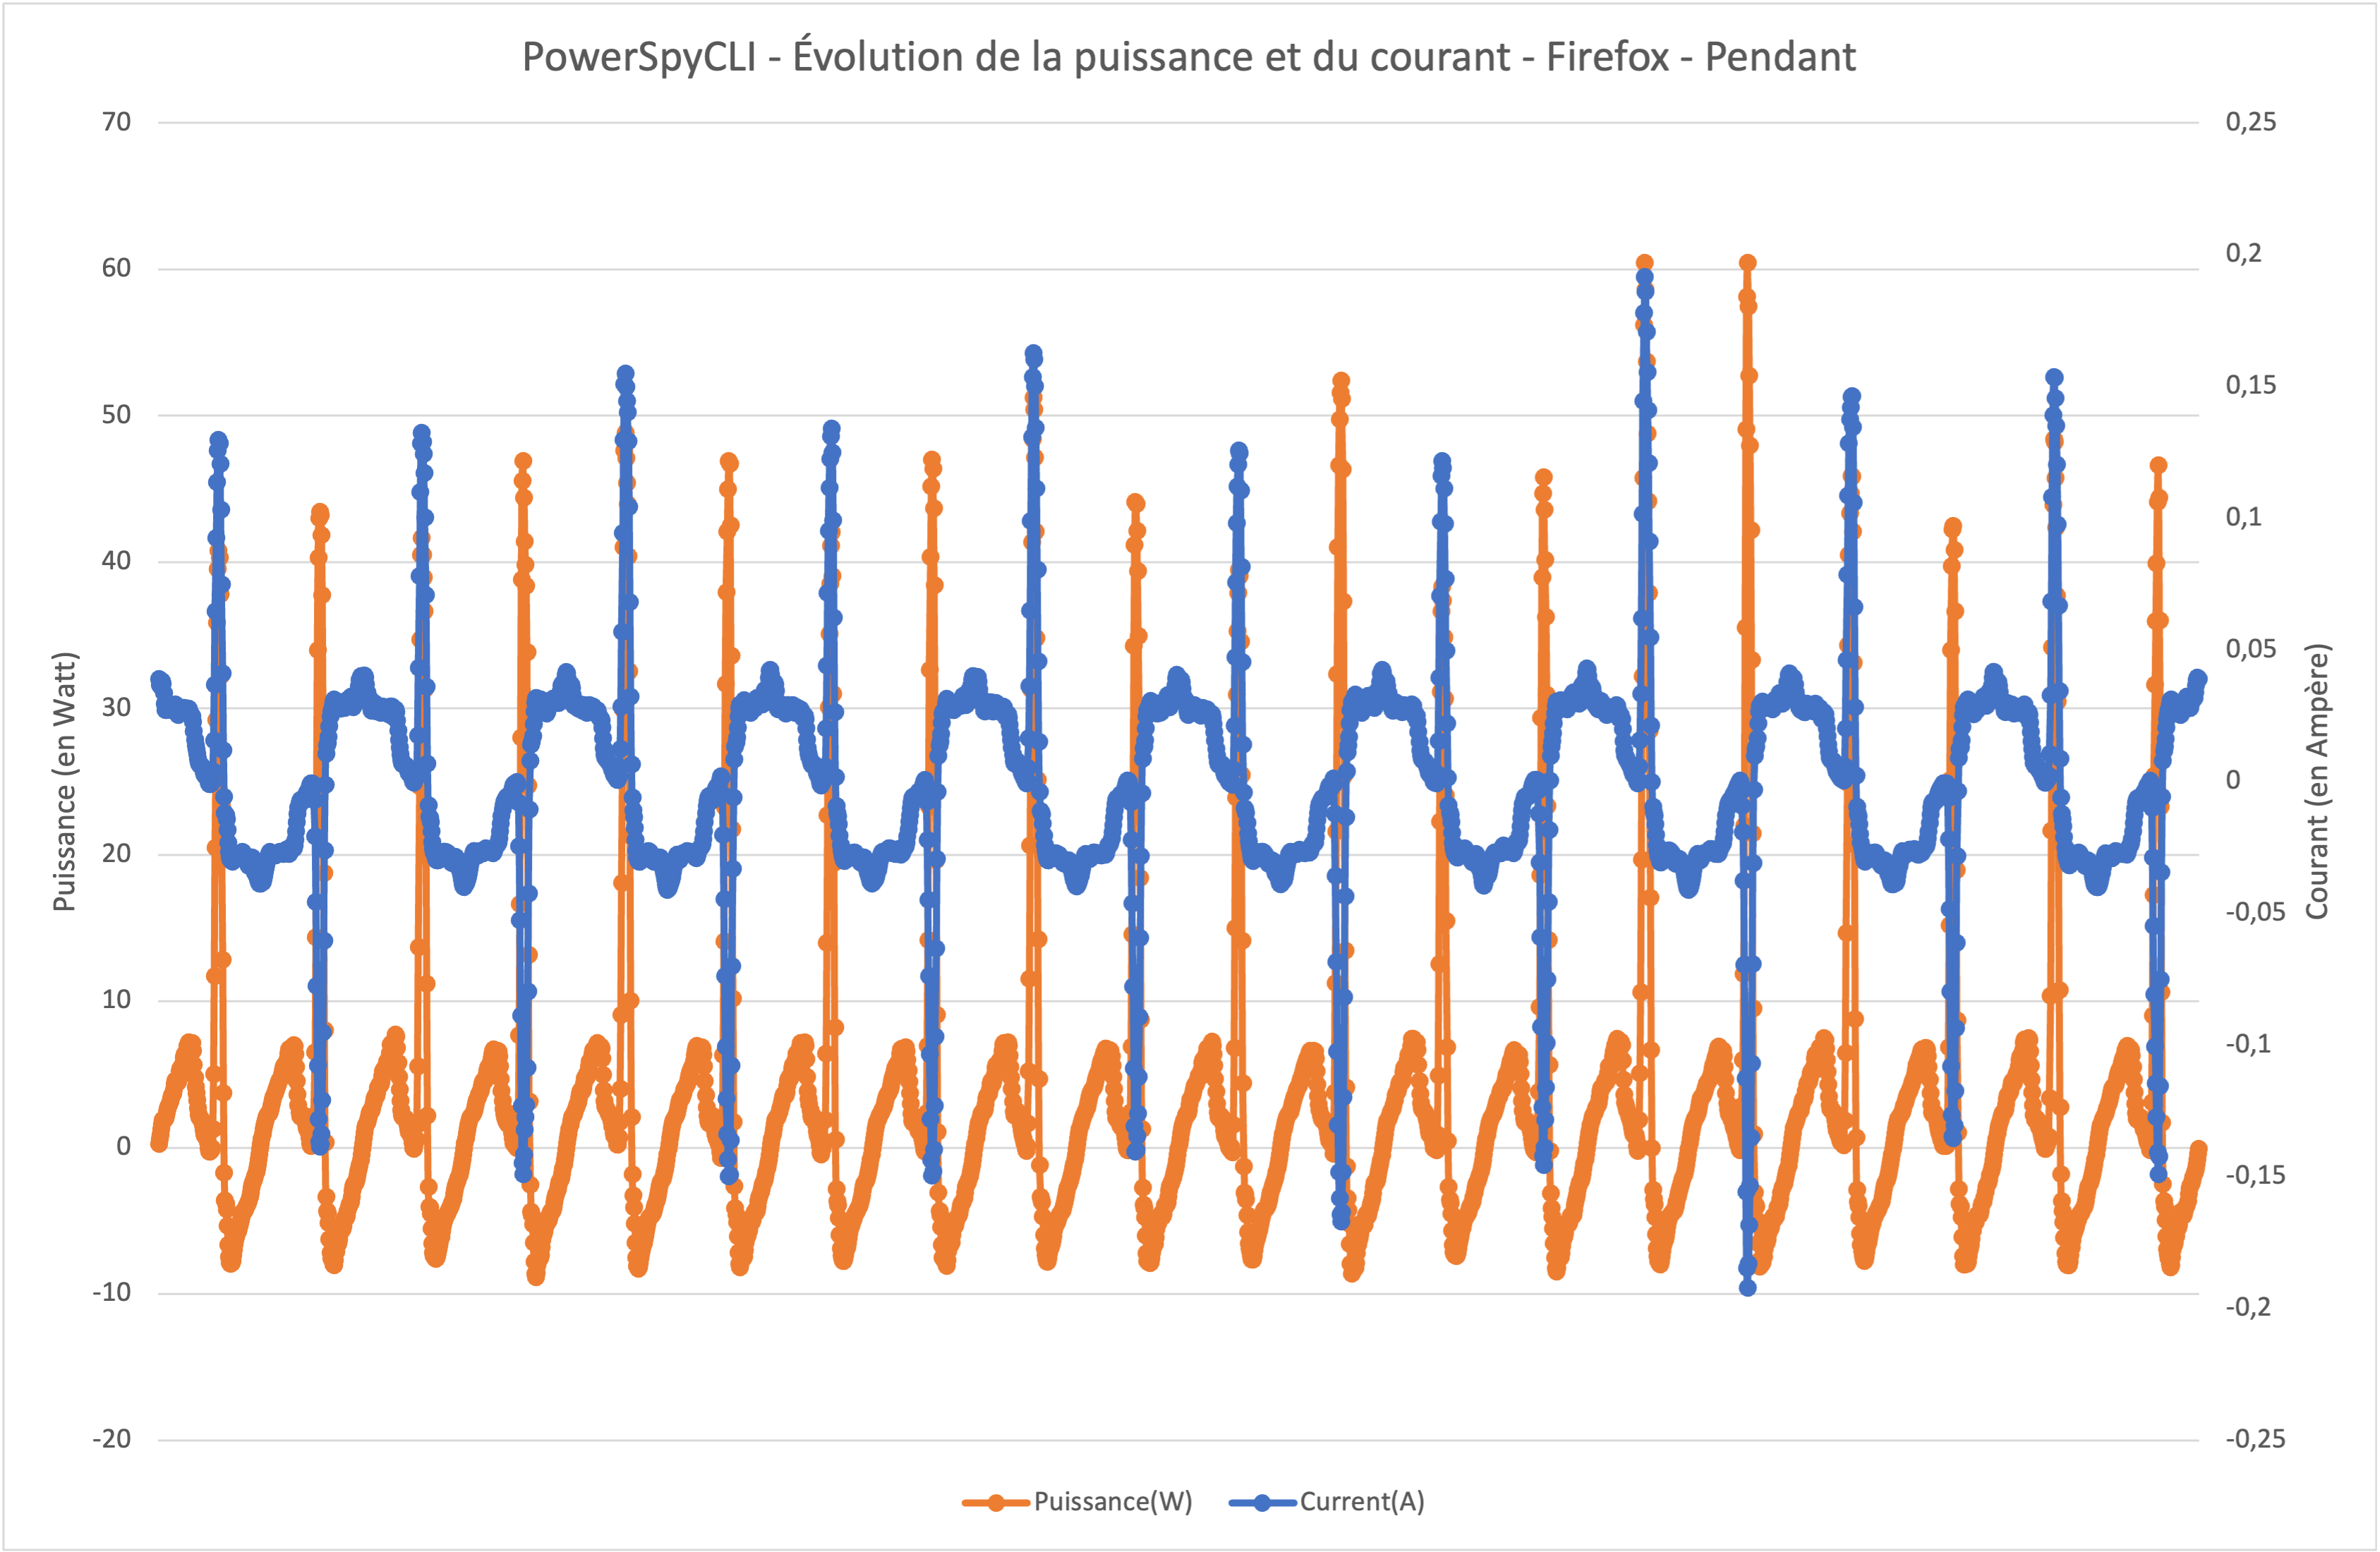
\includegraphics[width=1\linewidth]{res//graph/PowerSpyCLI/Puissance_ff_pendant.png}
    \caption{PowerSpyCLI - Puissance - Firefox - \textit{during}}
    \label{fig:pscli_power_ff_after}
\end{figure}
\begin{figure}[H]
    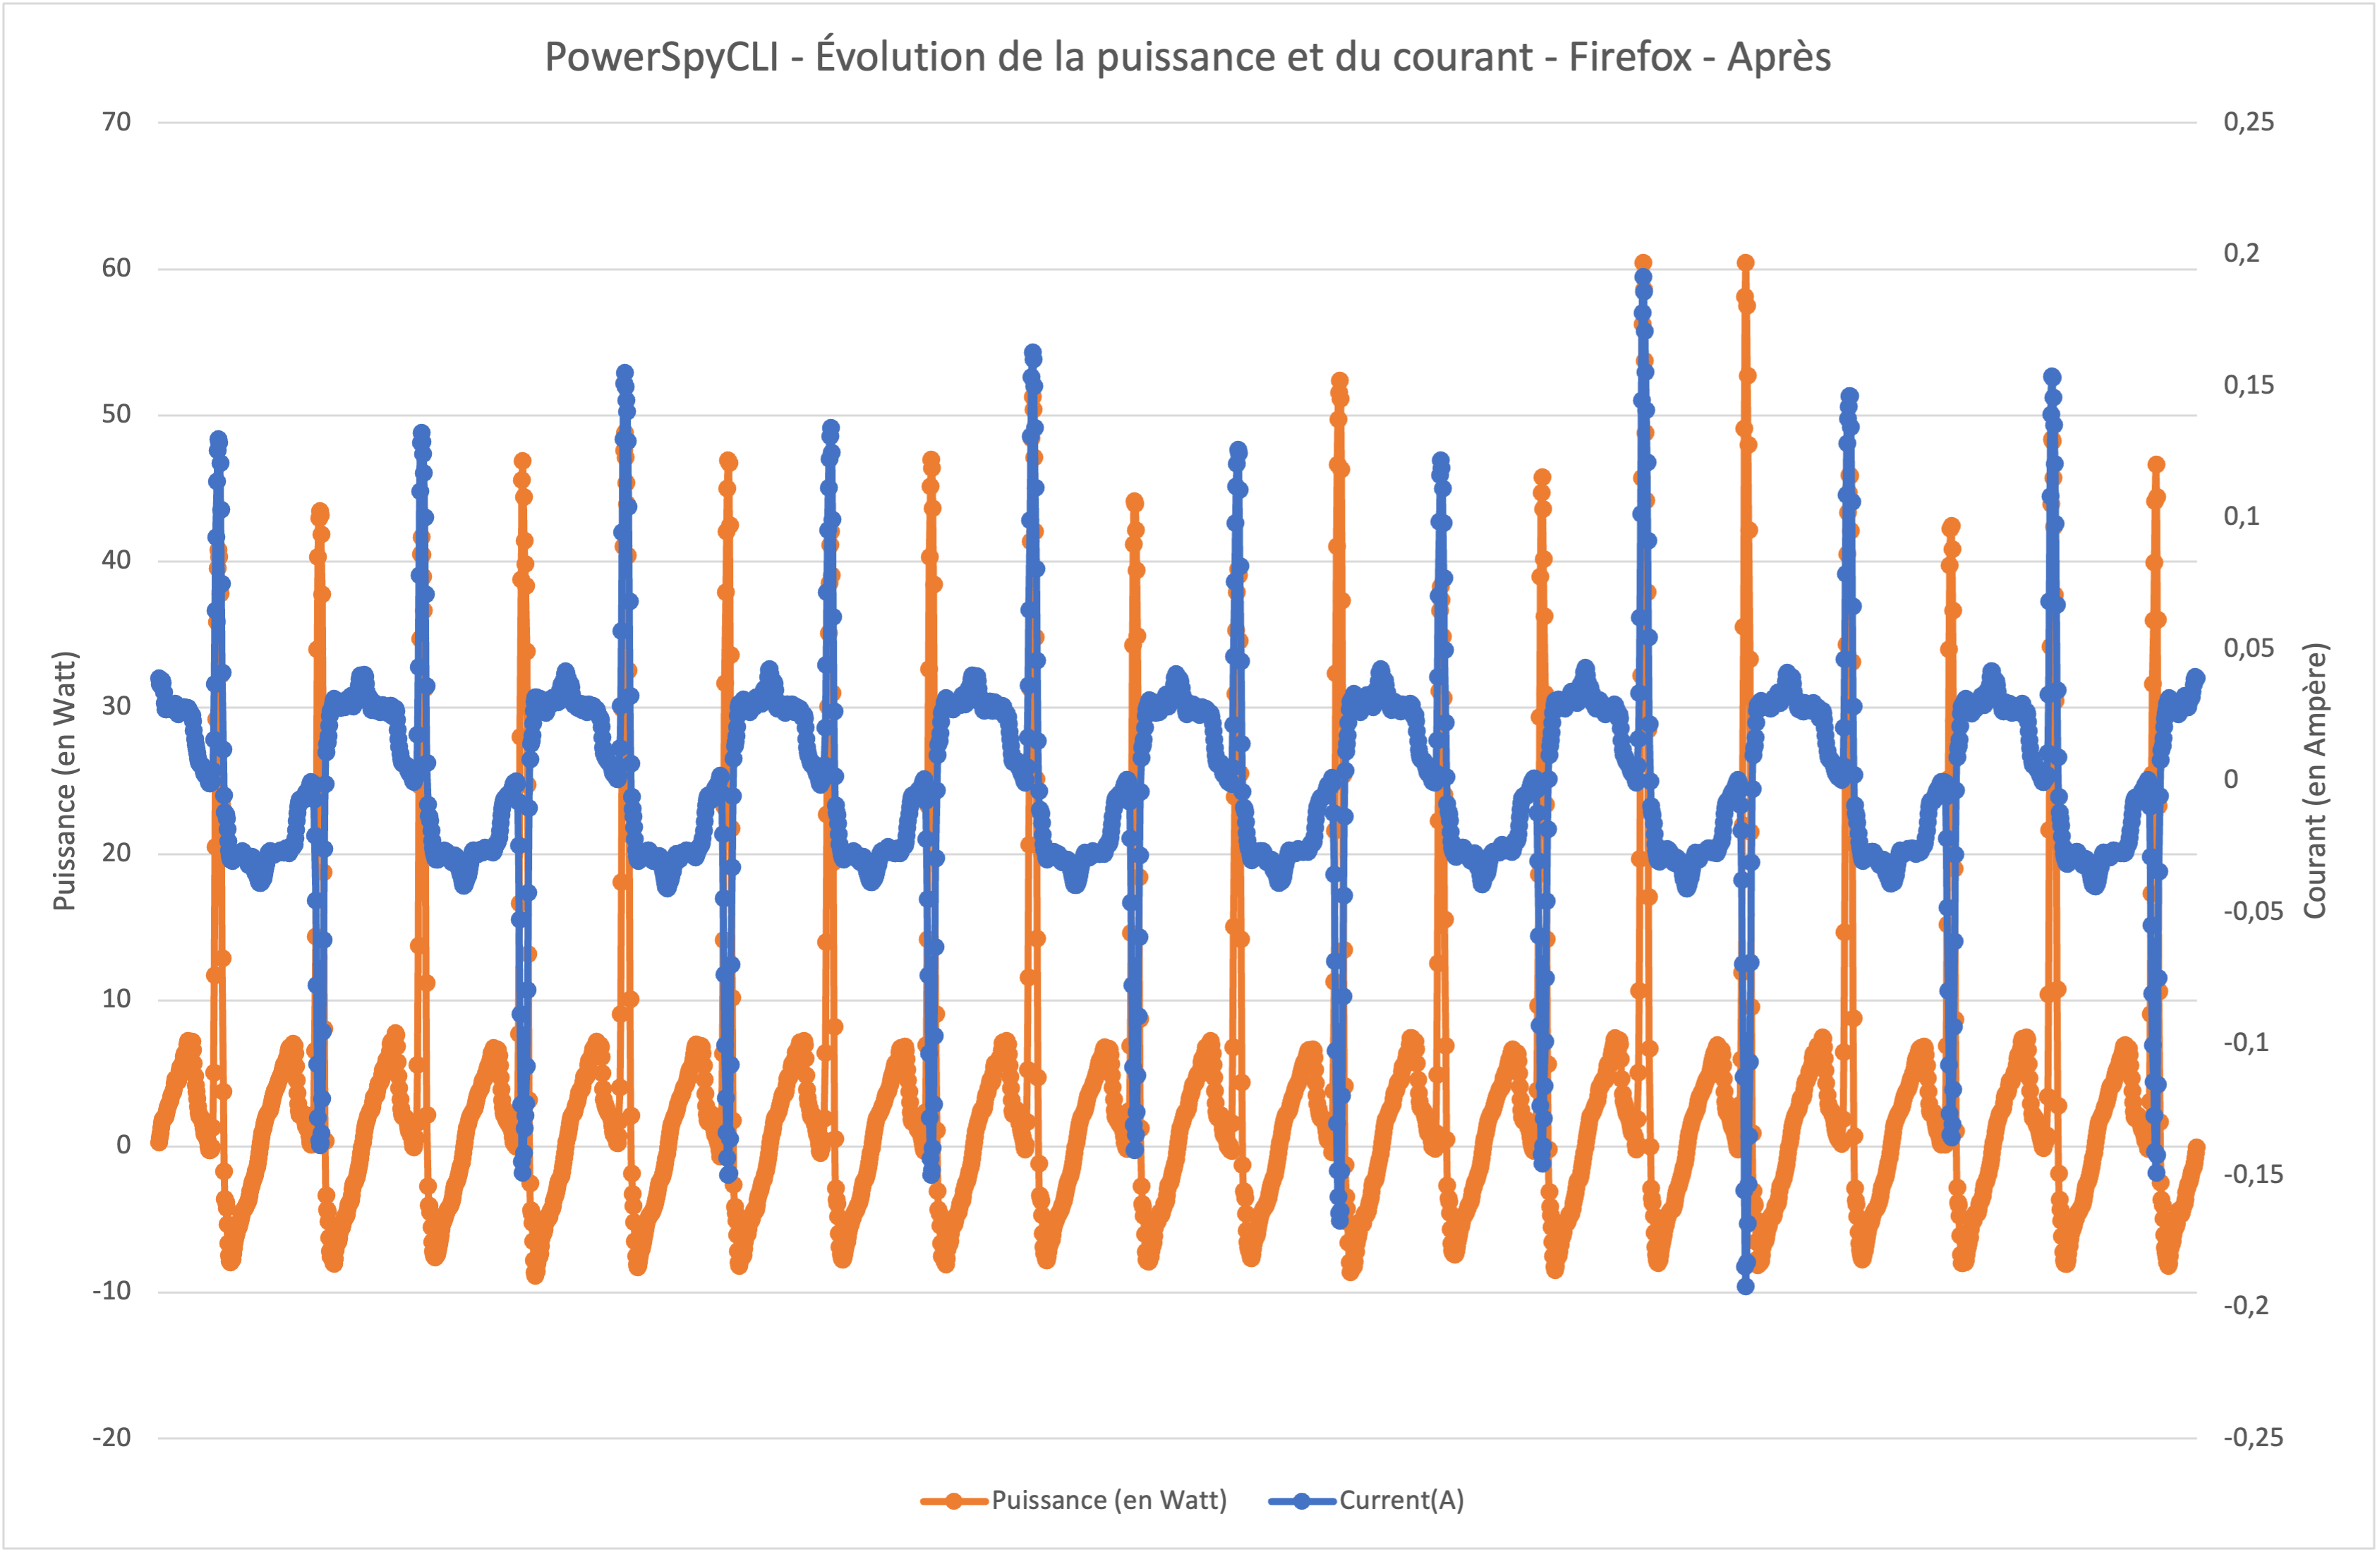
\includegraphics[width=1\linewidth]{res//graph/PowerSpyCLI/Puissance_ff_apres.png}
    \caption{PowerSpyCLI - Puissance - Firefox - \textit{after}}
    \label{fig:pscli_power_ff_after}
\end{figure}


Comme nous pouvons le remarquer, pour tous les six graphiques, peu de différence sont notable entre les différentes parties (avant, pendant, après) de l'expérience. En effet, sur Linux, l'utilisation du CPU et la consommation sembles beaucoup plus cohérent que sur Windows. Mis à part la présence de pics sur les courbes représentant le courant, et qui peuvent être expliqué très simplement par la physique elle même, et non pas le côté logiciel, nous ne pouvons pas remarquer une grande différence.
Les résultats sont aussi similaire à \ref{subsubsec:powerspycli} car il s'agit au fond du même Software, la version CLI proposant juste accès aux fonctionnalités à travers la ligne de commande du terminal et PowerSpy2 laissant accès à ces mêmes fonctionnalités à travers un GUI.

\subsubsection{Power Joular}

\paragraph{
\textbf{Chrome}\newline
}
\begin{figure}[H]
    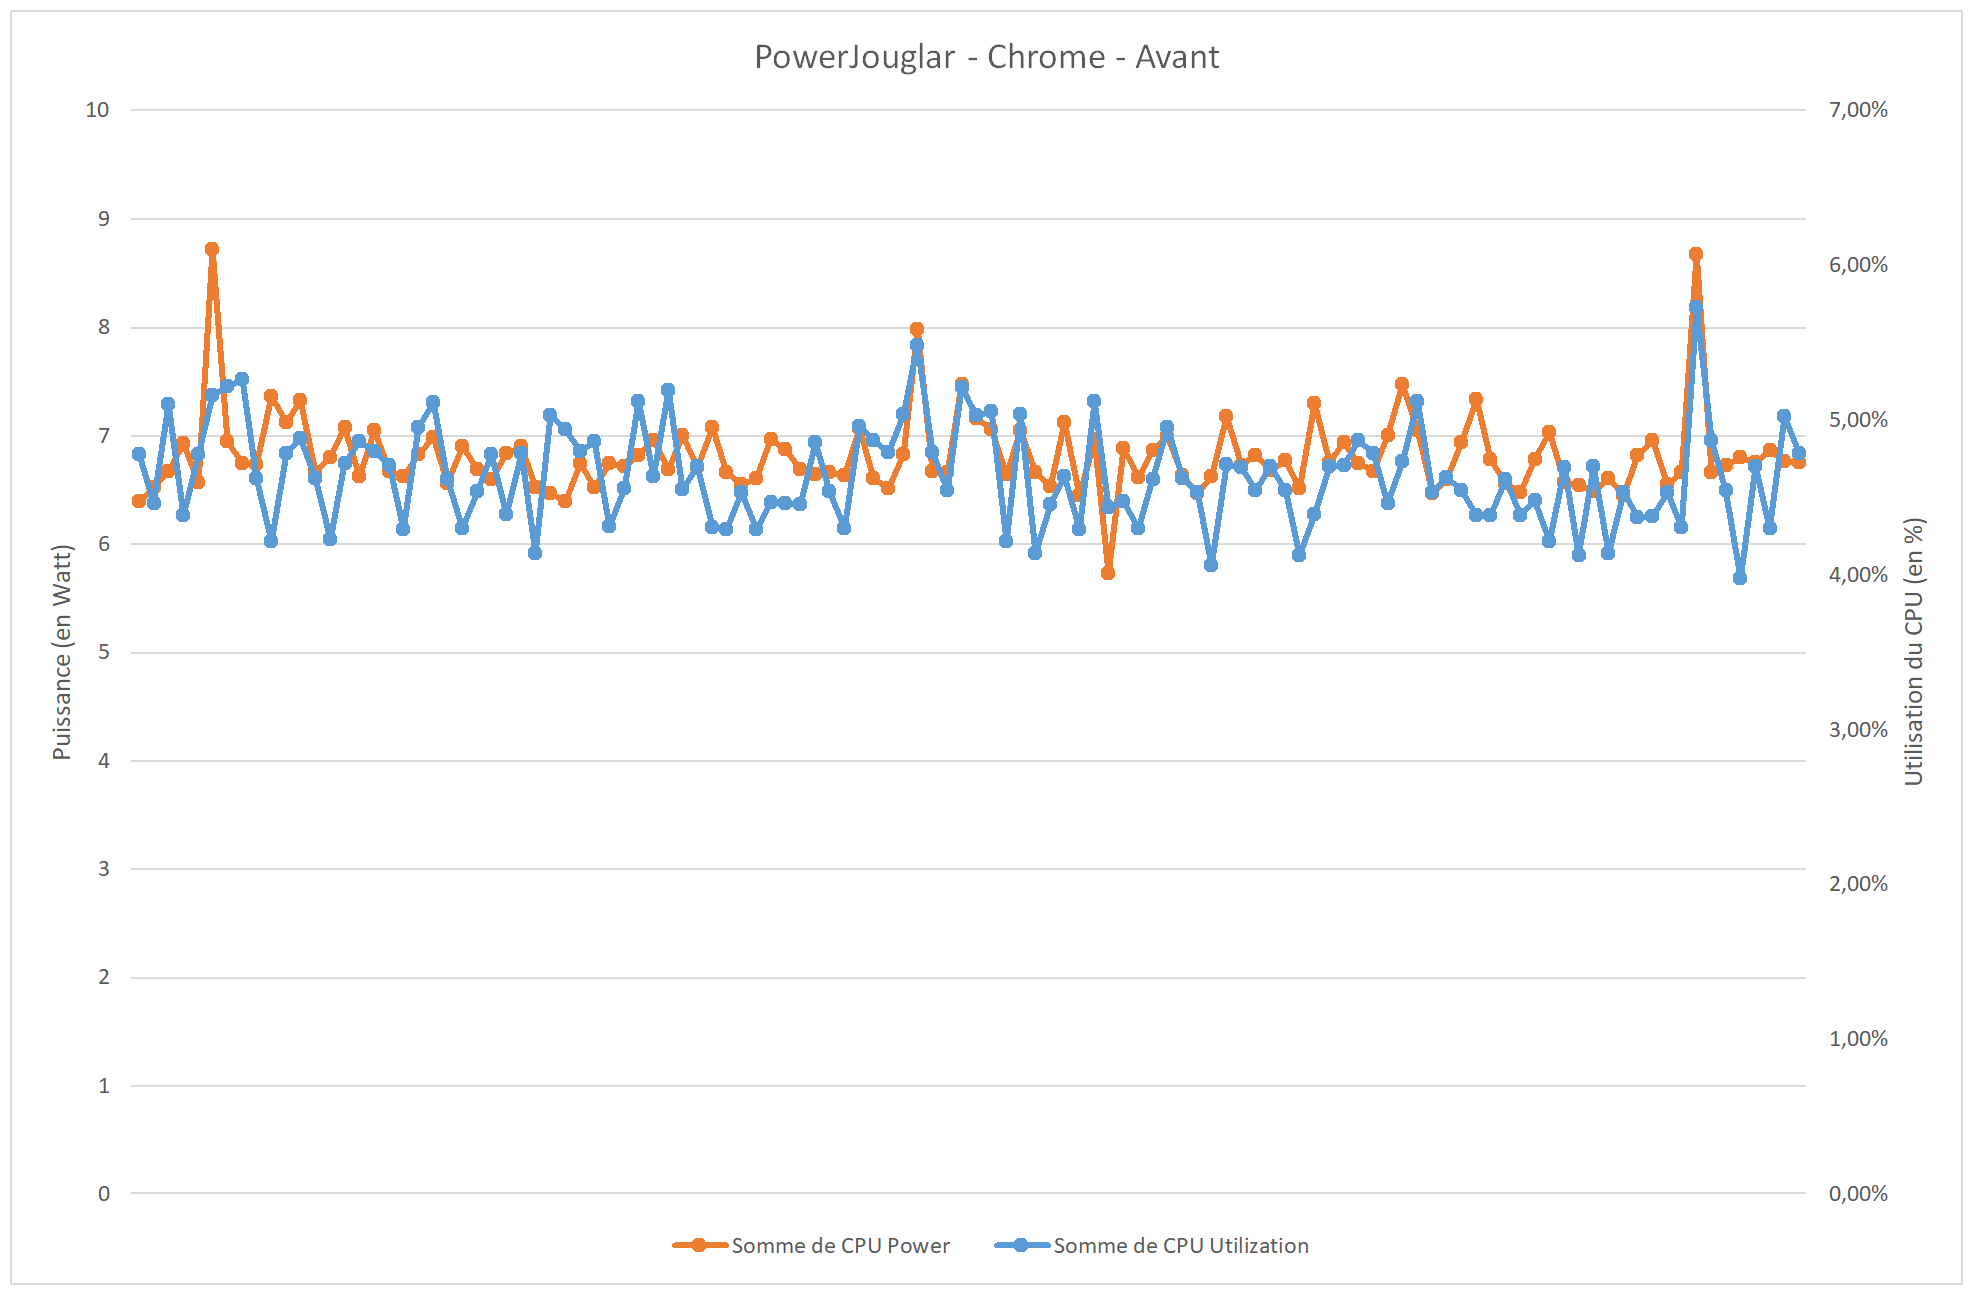
\includegraphics[width=1\linewidth]{res//graph/PowerJoular/chrome-avant.png}
    \caption{PowerJoular - Chrome - \textit{before}}
    \label{fig:pj_chrome_before}
\end{figure}
\begin{figure}[H]
    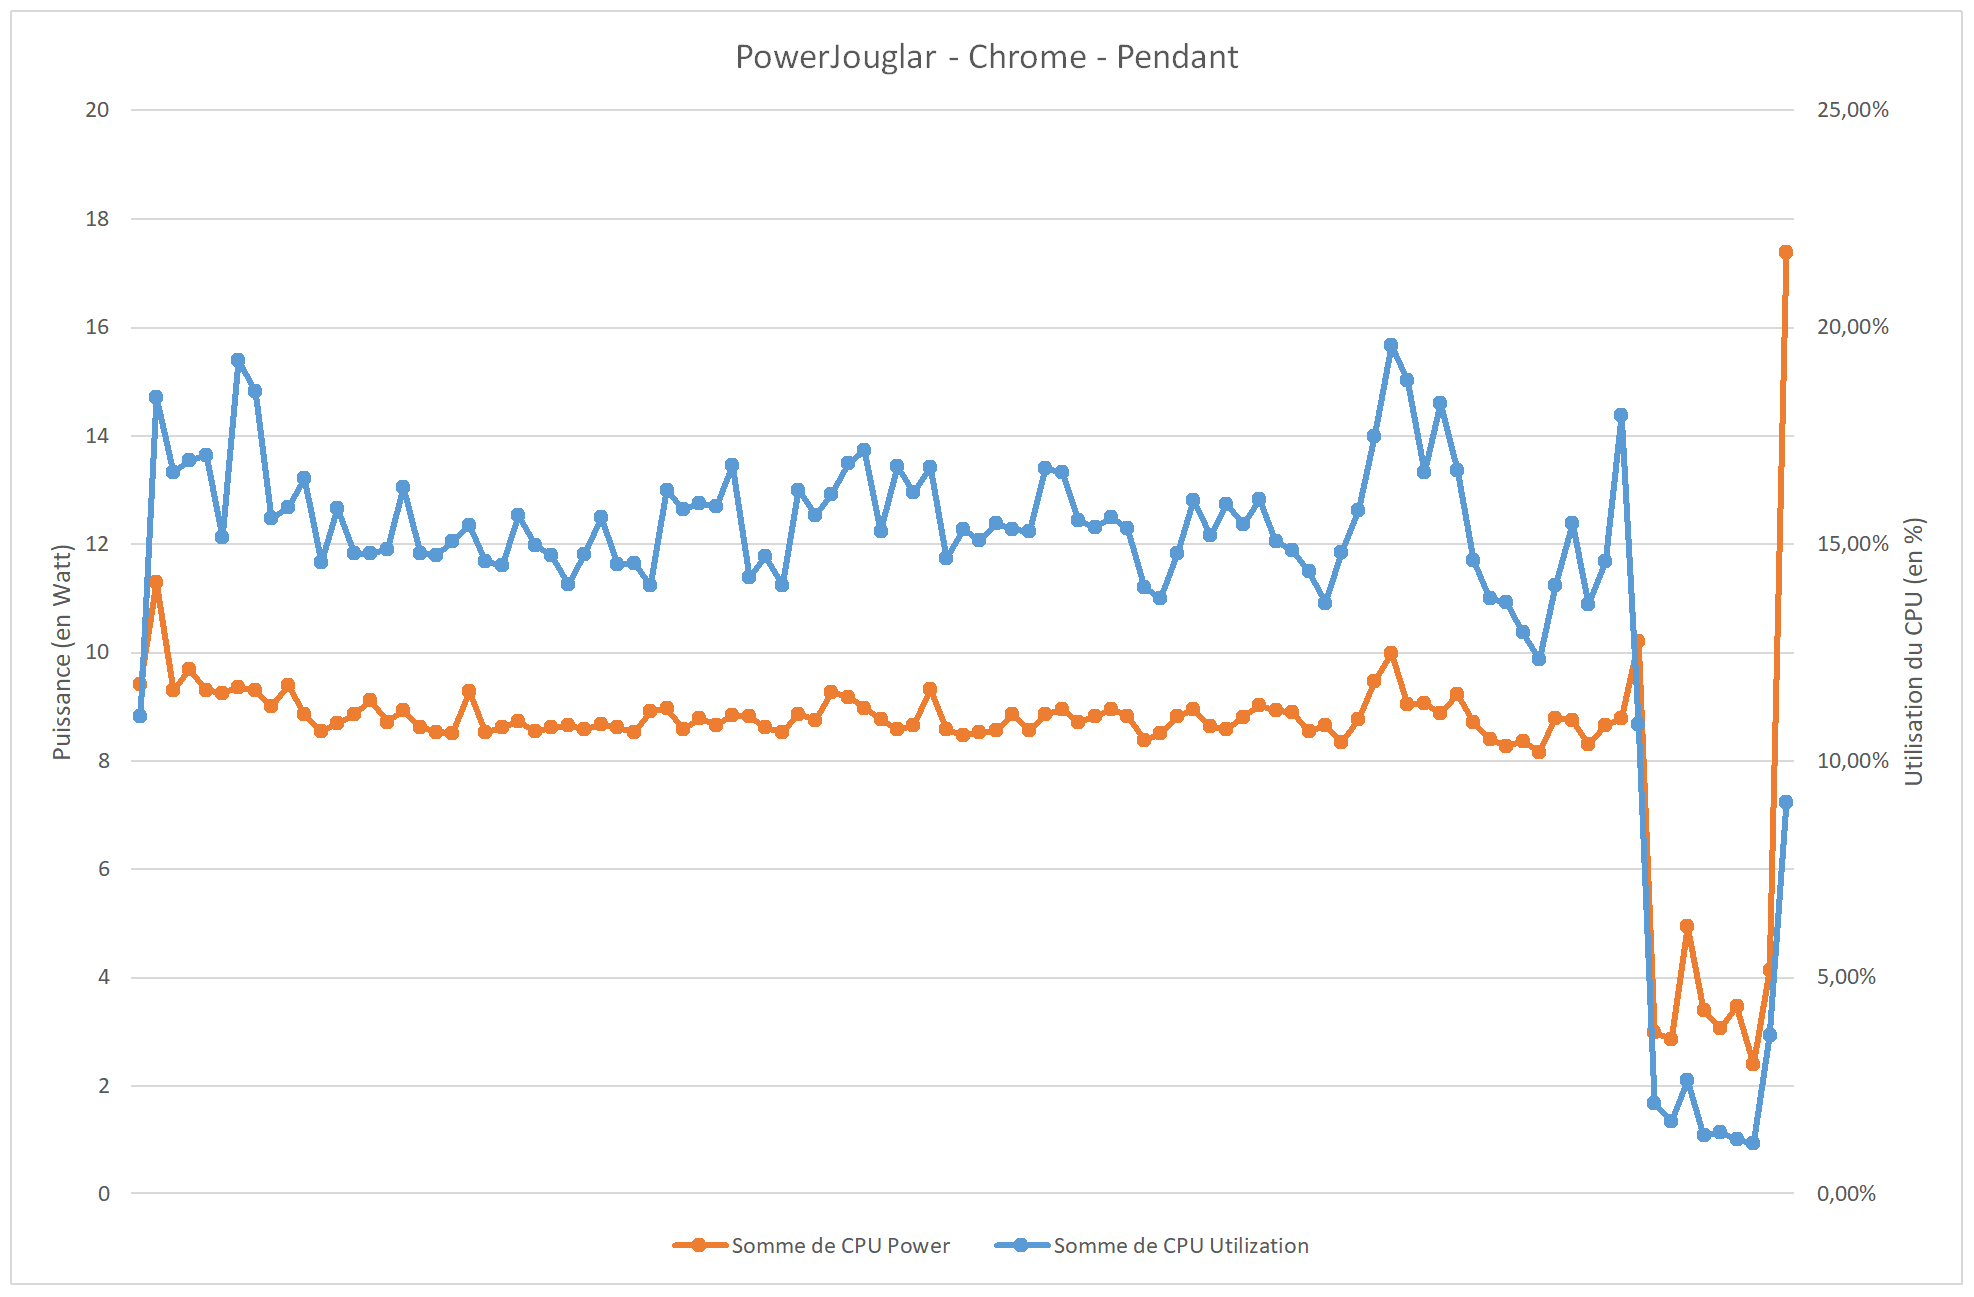
\includegraphics[width=1\linewidth]{res//graph/PowerJoular/chrome-during.png}
    \caption{PowerJoular - Chrome - \textit{during}}
    \label{fig:pj_chrome_during}
\end{figure}
\begin{figure}[H]
    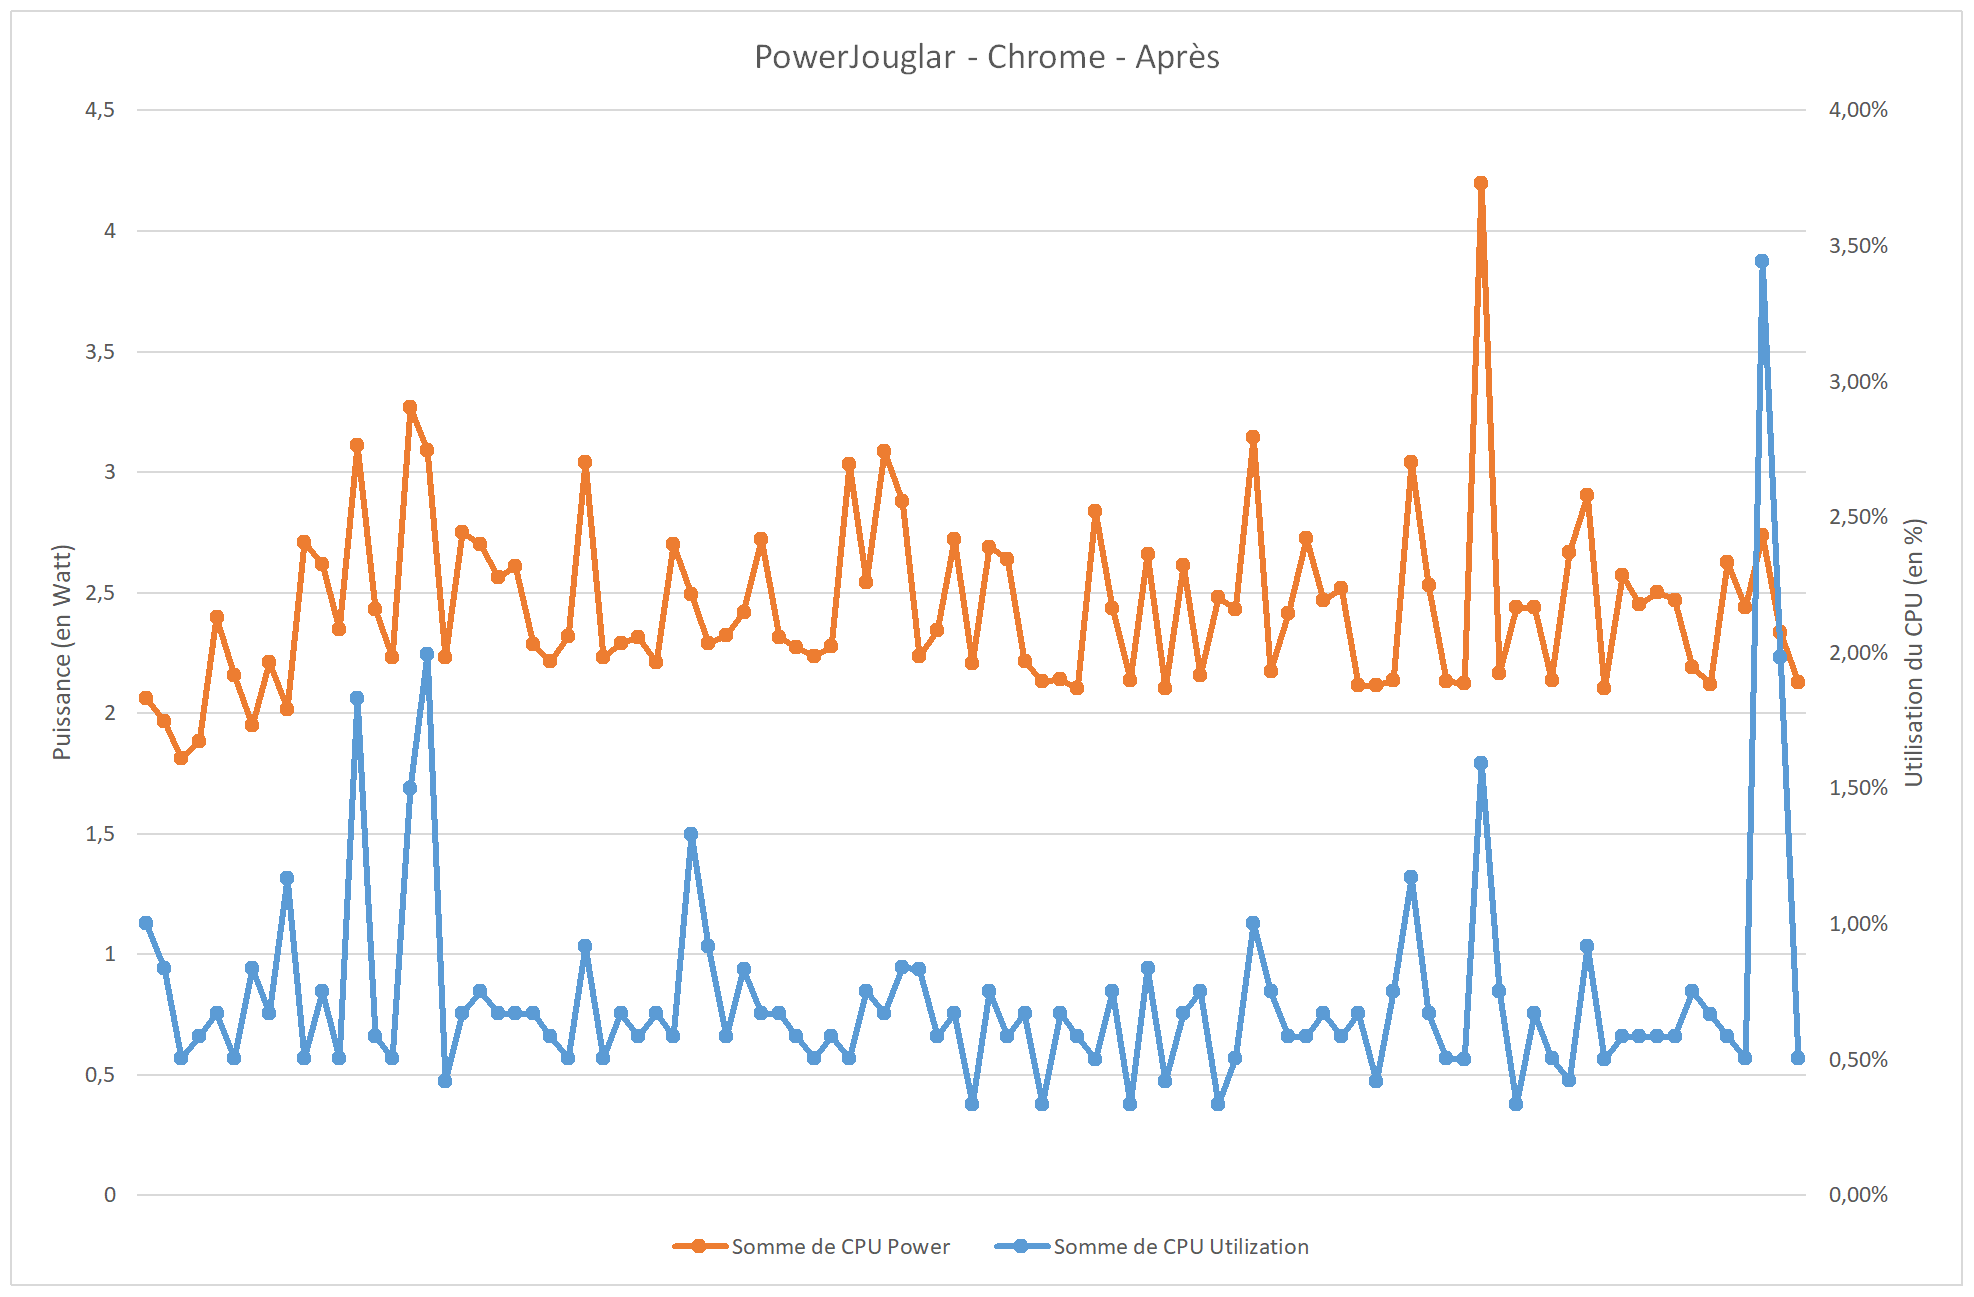
\includegraphics[width=1\linewidth]{res//graph/PowerJoular/chrome-after.png}
    \caption{PowerJoular - Chrome - \textit{after}}
    \label{fig:pj_chrome_after}
\end{figure}
Une première chose intéressante à noter, et nous verrons avec Firefox s'il s'agit d'une particularité de Chrome ou si le fonctionnement de Linux y est pour quelque chose. Le pourcentage d'utilisation et donc la consomation énergétique augmente bien évidemment lors de la lecture de la vidéo. Cependant, le pourcentage semble, selon PowerJoular, baisser jusqu'à 1\% de l'utilisation du CPU mais la consomation énergétique reste "élevé" à environ 2.5 W.
De plus, comparé à Windows et Intel Power Gadget \ref{subsubsec:chrome_ipg}, nous pouvons voir que sur Linux, Chrome semble moins stable. Nous pouvons observer beaucoup plus de flucutations et de pics, que ce soit au niveau du pourcentage d'utilisation ou de la puissance consomée. 
Dans tous les cas, mis à part la partie \textit{after}, le pourcentage et la puissance sont coléré et se suivent.


\paragraph{
\textbf{Firefox}\newline}
\begin{figure}[H]
    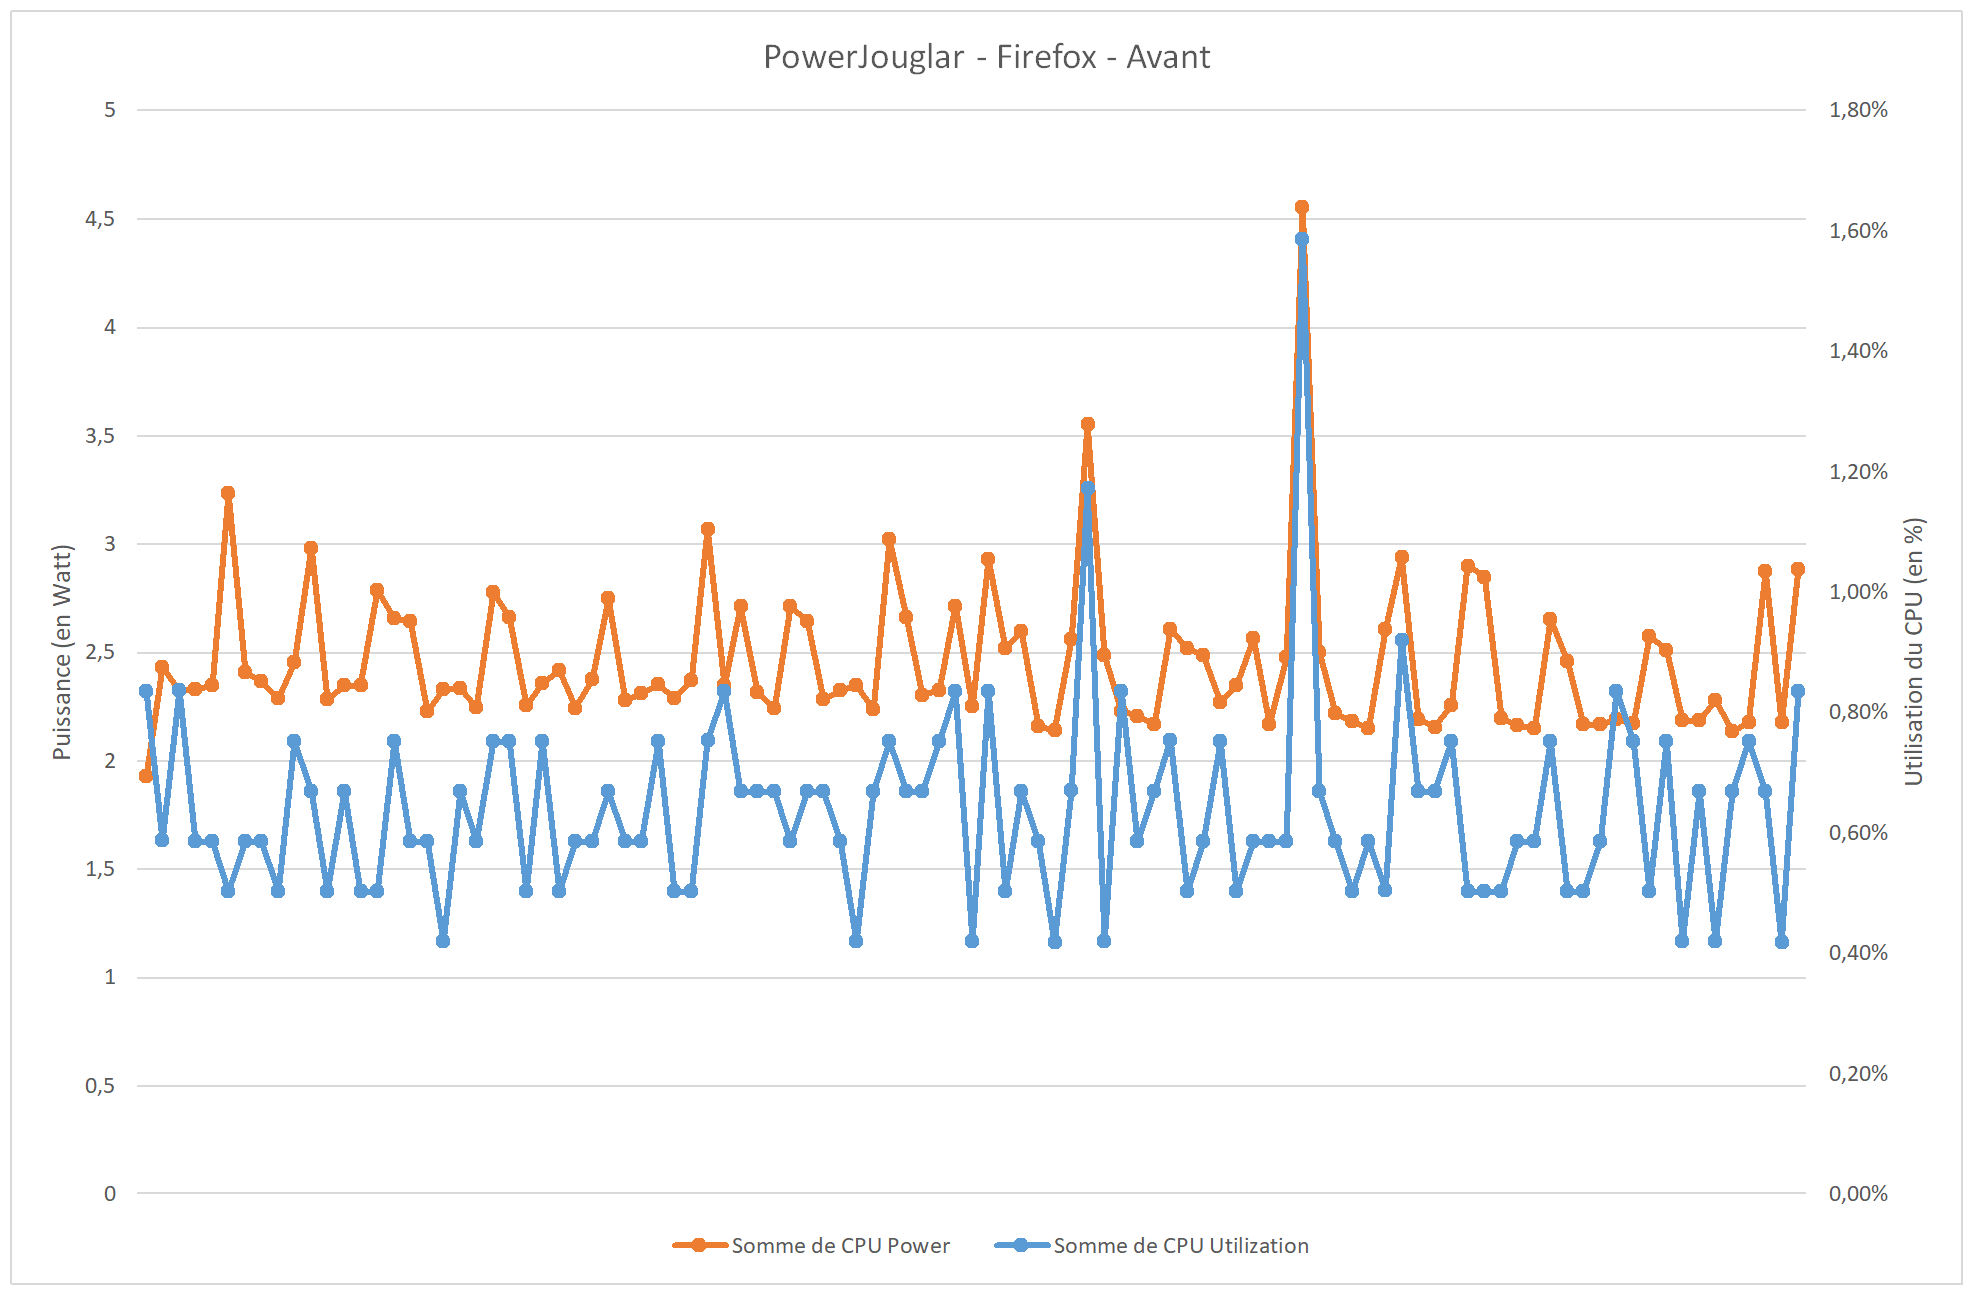
\includegraphics[width=1\linewidth]{res//graph/PowerJoular/ff-avant.png}
    \caption{PowerJoular - Firefox - \textit{before}}
    \label{fig:pj_ff_before}
\end{figure}
\begin{figure}[H]
    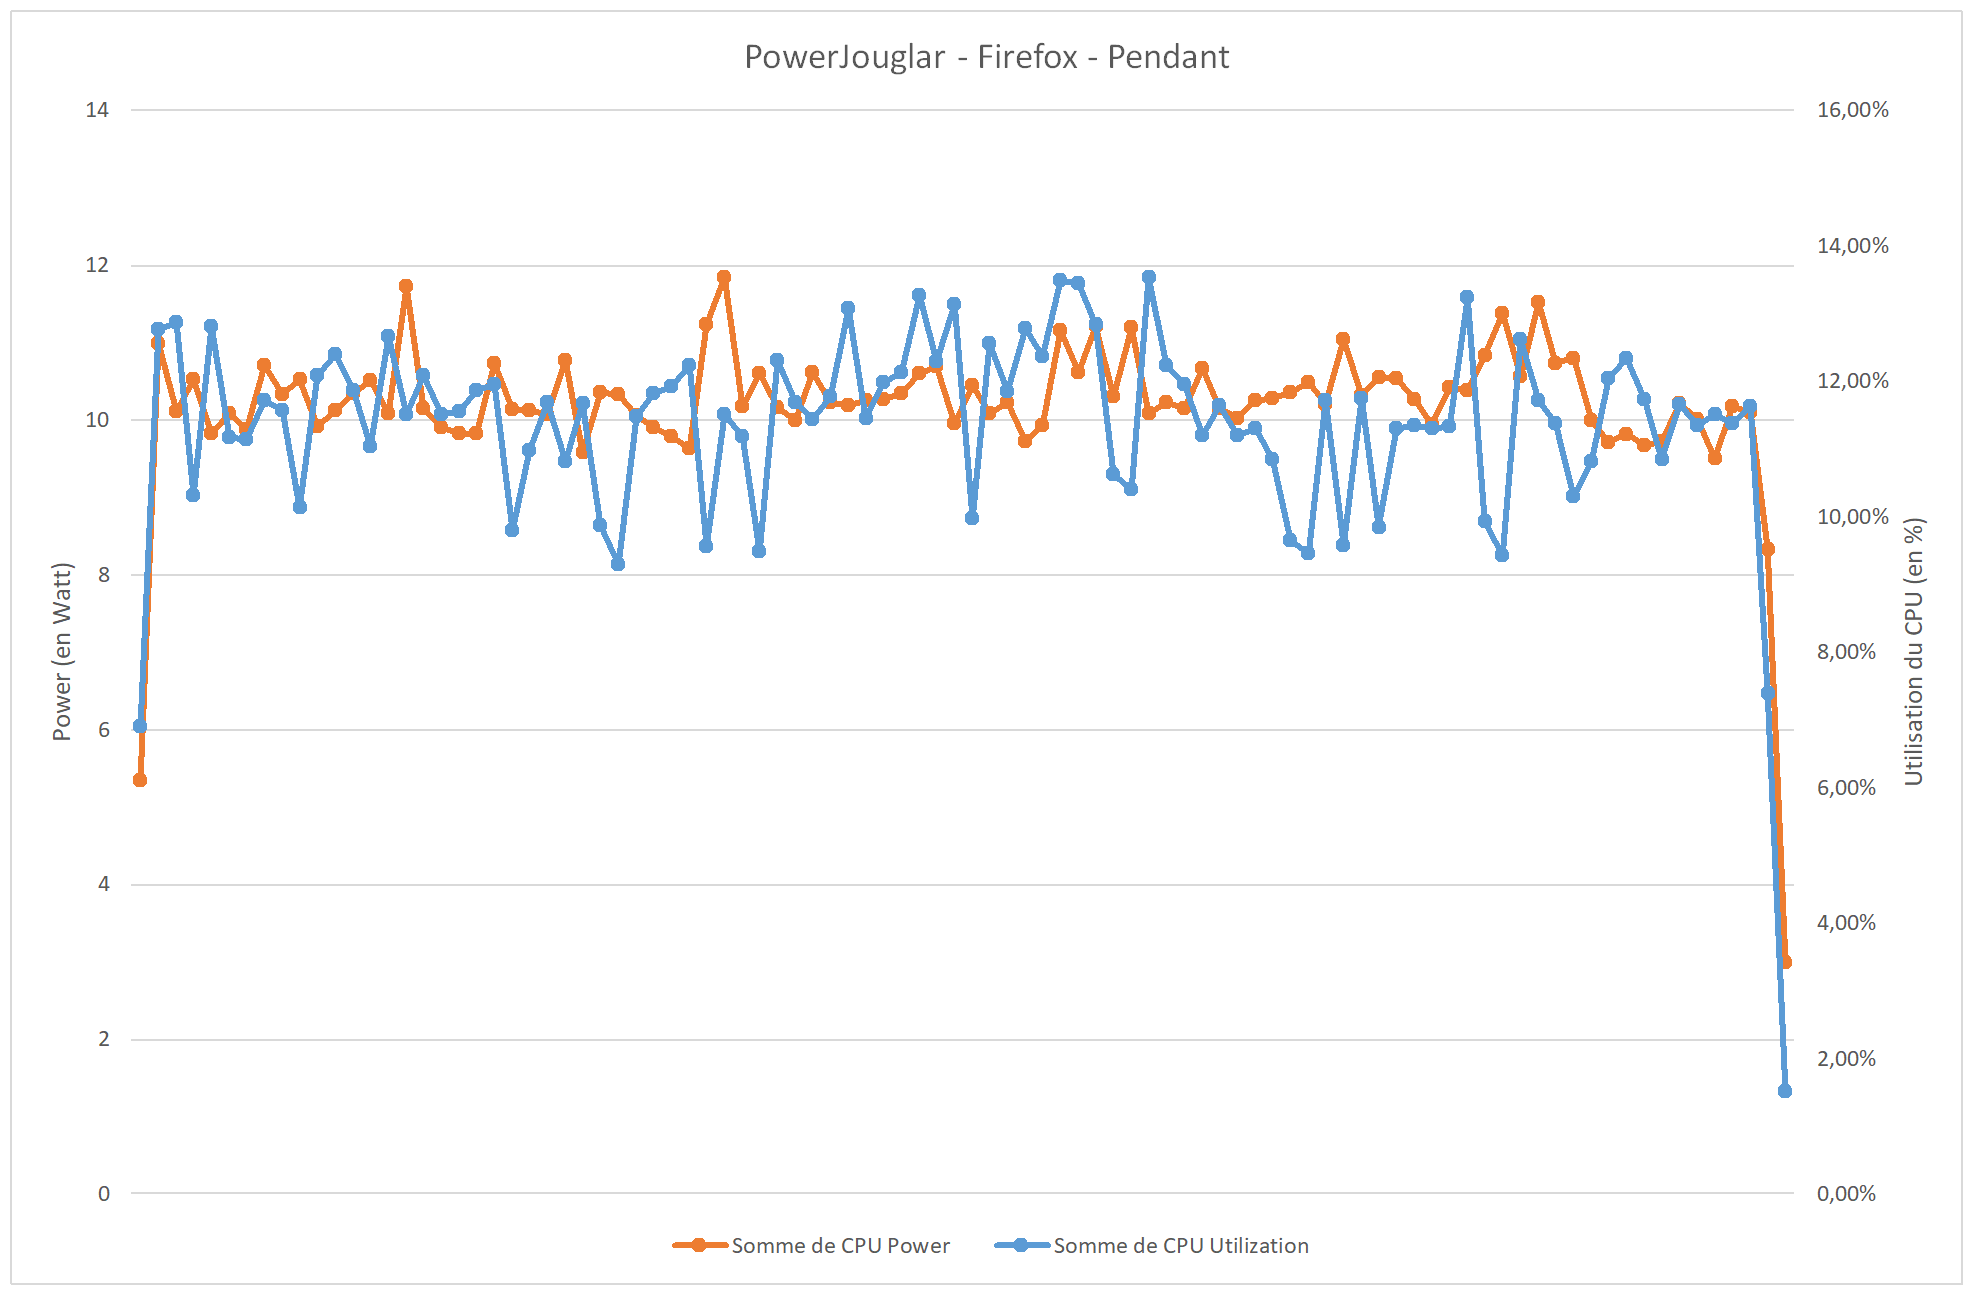
\includegraphics[width=1\linewidth]{res//graph/PowerJoular/ff-during.png}
    \caption{PowerJoular - Firefox - \textit{during}}
    \label{fig:pj_ff_during}
\end{figure}
\begin{figure}[H]
    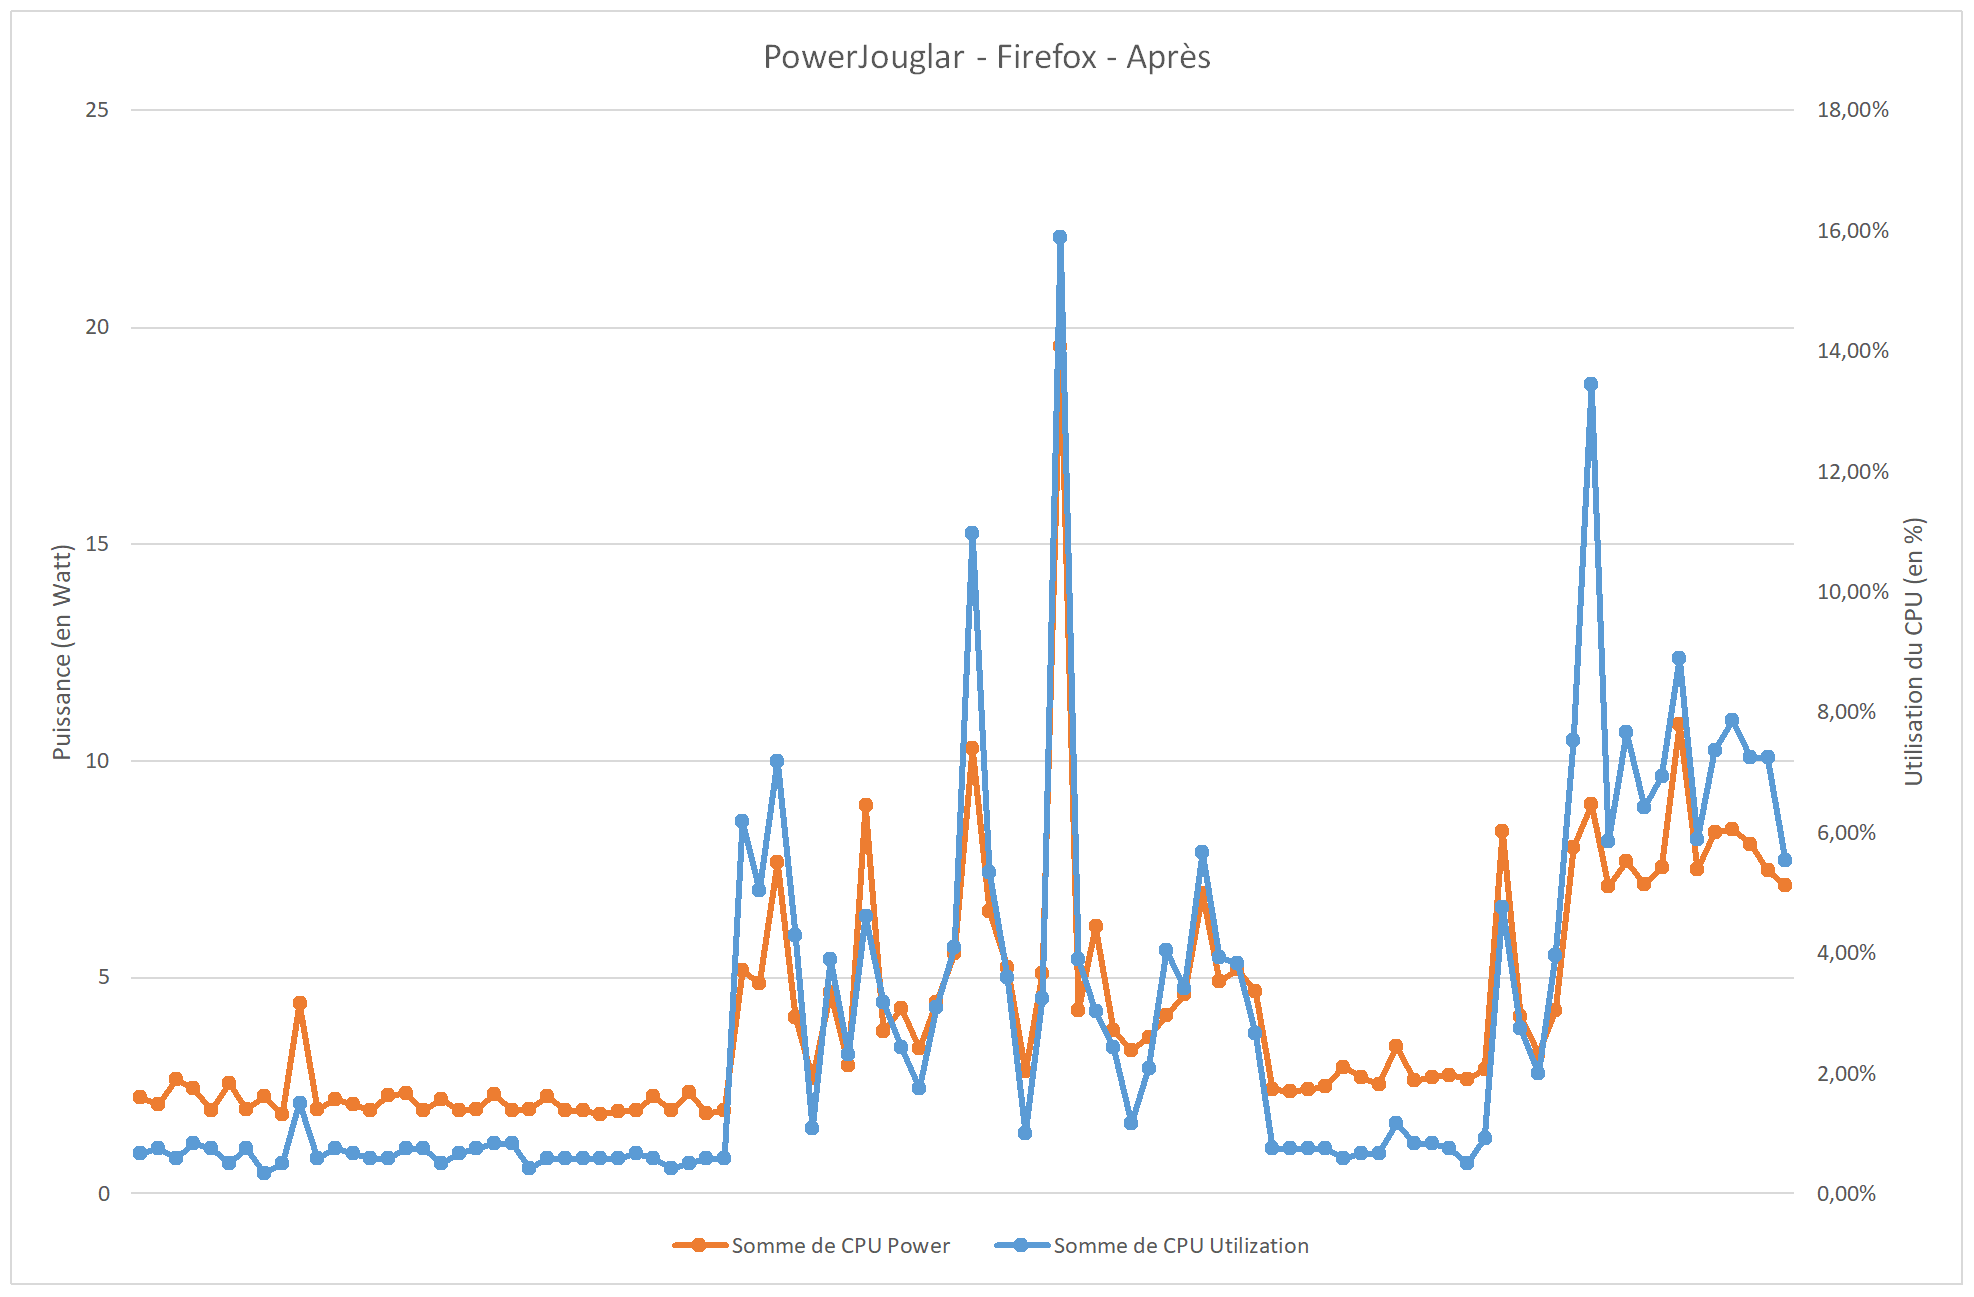
\includegraphics[width=1\linewidth]{res//graph/PowerJoular/ff-after.png}
    \caption{PowerJoular - Firefox - \textit{after}}
    \label{fig:pj_ff_after}
\end{figure}
La première remarque, et pour faire un parallèle avec l'expérience fait sur Chrome, nous pouvons voir que l'anomalie qui se produit sur la période \textit{after} n'est pas présente ici. La puissance suit le pourcentage d'utilisation et celle-ci ne reste pas supérieur que ce qui devraity logiquement rester. 
Pour le reste, les variables suivent des évolution logiques. 

\paragraph{Pour conclure sur PowerJoular, lors de la lecture de la vidéo, Chrome semble une nouvelle fois le meilleur élève comparé aux autres (ici Firefox). Avec une légère baisse sur l'utilisation du CPU, ainsi que sur la puissance. Mais comparé à Windows ou à nos autres tests, ces différences sont moindres entre les deux naviguateurs.
Cependant, lors des tests faits avant le lancement de la vidéo, Firefox est le meilleur des deux sur une plus large marge. En effet, avec seulement moins de 1\% d'utilisation du CPU pour une moyenne de 2.5W de consommation contre 5\% et une moyenne de 7W pour Chrome, il semblerait plus efficace d'utiliser Firefox hors des utilisations nécessitant plus de calcul graphique (utilisation du GPU). }

\chapter{\centering Discussion}
\subsection{Avantages et inconvénients des différents navigateurs en termes de consommation énergétique}
Comme ont pu nous le montrer les différentes expériences sur les différents naviguateurs (sur différents OS), nous avons pu déterminer une liste des naviguateur à basse consommation. Cette liste part de 1 : le moins consommateur jusqu'à x %TODO: modifier x par le nombre de naviguateur testé
le plus consommateur.
\begin{enumerate}
    \item Firefox
    \item Chrome
    \item Edge
\end{enumerate}

\subsection{Fiabilité des outils de mesure utilisés}

La fiabilité des outils de mesure utilisés dans nos tests de consommation d'énergie est cruciale pour garantir des résultats précis et significatifs. Voici une évaluation de la fiabilité des outils spécifiques employés dans notre étude :

\begin{itemize}
    \item {\bfseries Intel Power Gadget (Windows) :} Intel Power Gadget est une application fiable pour mesurer la consommation d'énergie du CPU sur les systèmes Windows. Il offre des données en temps réel et est largement utilisé pour des analyses de performance énergétique.

    \item {\bfseries Wattmètre (Linux) :} La mesure de la consommation d'énergie avec un wattmètre est une méthode directe et fiable. Cependant, la précision dépend de la qualité du wattmètre utilisé.

    \item {\bfseries PowerSpy CLI, PowerSpy2, PowerJoular (Linux) :}  Ces outils logiciels sont utilisés pour leur capacité à fournir des informations détaillées sur la consommation d'énergie du CPU sous Linux. Ils sont couramment utilisés dans des scénarios similaires et sont considérés comme fiables dans la communauté de recherche.
    
\end{itemize}

En conclusion, la fiabilité des outils de mesure, tels qu'Intel Power Gadget, le wattmètre, PowerSpy CLI, PowerSpy2, PowerJoular, VLC, et QuickTime Player, a été primordiale pour assurer des résultats précis et cohérents. Ces outils, reconnus dans leurs domaines respectifs, ont contribué à une évaluation fiable de la consommation d'énergie des navigateurs et des lecteurs vidéos. L'approche avant, pendant, et après la lecture de la vidéo renforce la solidité de nos résultats, offrant ainsi une base solide pour une analyse comparative fiable des performances énergétiques.


\subsection{Limitations de l'étude et pistes pour des recherches futures}
L'étude s'étend sur différents OS, utilisant différents outils pour différents naviguateurs, mais les expériences ont étaient réalisés de manière assez simple avec une possible manque de rigueur. De plus, la difficulté logistique et matériel que nous avons pu rencontré rends l'étude moins fiable scientifiquement. 
Un meilleur environnement de test, avec un protocol claire, établie, suivie et respecté serait un très bon moyen d'améliorer notre étude. 

\chapter{\centering Conclusion}


En conclusion, l'optimisation de la consommation d'énergie des navigateurs web représente un aspect crucial de la gestion efficace des ressources informatiques. En adoptant des pratiques telles que les mises à jour régulières, la limitation des extensions, la gestion judicieuse des onglets, l'activation des modes économes en énergie, et en favorisant des navigateurs réputés pour leur faible consommation d'énergie comme Chrome, les utilisateurs peuvent contribuer à une utilisation plus responsable et durable de leurs dispositifs. La sensibilisation à ces pratiques simples, combinée à la mise en œuvre de mesures d'efficacité énergétique, est essentielle pour créer un environnement numérique plus économe en énergie et respectueux de l'environnement.

\end{document}